% Soubory musí být v kódování, které je nastaveno v příkazu \usepackage[...]{inputenc}

\documentclass[%
%  draft,    				  % Testovací překlad
  12pt,       				% Velikost základního písma je 12 bodů
  a4paper,    				% Formát papíru je A4
%  oneside,      			% Jednostranný tisk (výchozí)
%% Z následujicich voleb lze použít maximálně jednu:
%	dvipdfm  						% výstup bude zpracován programem 'dvipdfm' do PDF
%	dvips	  						% výstup bude zpracován programem 'dvips' do PS
%	pdftex							% překlad bude proveden programem 'pdftex' do PDF (výchozí)
	unicode,						% Záložky a metainformace budou v kódování unicode
]{report}				    	% Dokument třídy 'zpráva'

\usepackage[utf8]		%	Kódování zdrojových souborů je UTF-8
	{inputenc}					% Balíček pro nastavení kódování zdrojových souborů

\usepackage[				% Nastavení okrajů
	bindingoffset=10mm,		% Hřbet pro vazbu
	hmargin={25mm,25mm},	% Vnitřní a vnější okraj
	vmargin={25mm,34mm},	% Horní a dolní okraj
	footskip=17mm,			% Velikost zápatí
	nohead,					% Bez záhlaví
	marginparsep=2mm,		% Vzdálenost poznámek u okraje
	marginparwidth=18mm,	% Šířka poznámek u okraje
]{geometry}

\usepackage{sectsty}
	%přetypuje nadpisy všech úrovní na bezpatkové, kromě \chapter, která je přenastavena zvlášť v thesis.sty
	\allsectionsfont{\sffamily}


\usepackage{graphicx} % Balíček 'graphicx' pro vkládání obrázků
											% Nutné pro vložení log školy a fakulty

\usepackage[
	nohyperlinks				% Nebudou tvořeny hypertextové odkazy do seznamu zkratek
]{acronym}						% Balíček 'acronym' pro sazby zkratek a symbolů
											% Nutné pro použití prostředí 'seznamzkratek' balíčku 'thesis'

\usepackage[
	breaklinks=true,		% Hypertextové odkazy mohou obsahovat zalomení řádku
	hypertexnames=false % Názvy hypertextových odkazů budou tvořeny
											% nezávisle na názvech TeXu
]{hyperref}						% Balíček 'hyperref' pro sazbu hypertextových odkazů
											% Nutné pro použití příkazu 'nastavenipdf' balíčku 'thesis'

\usepackage{pdfpages} % Balíček umožňující vkládat stránky z PDF souborů
                      % Nutné při vkládání titulních listů a zadání přímo
                      % ve formátu PDF z informačního systému

\usepackage{enumitem} % Balíček pro nastavení mezerování v odrážkách
  \setlist{topsep=0pt,partopsep=0pt,noitemsep}

\usepackage{cmap} 		% Balíček cmap zajišťuje, že PDF vytvořené `pdflatexem' je
											% plně "prohledávatelné" a "kopírovatelné"

\usepackage{upgreek}	% Balíček pro sazbu stojatých řeckých písmem
											%% např. stojaté pí: \uppi
											%% např. stojaté mí: \upmu (použitelné třeba v mikrometrech)
											%% pozor, grafická nekompatibilita s fonty typu Computer Modern!

\usepackage{dirtree}		% sazba adresářové struktury

\usepackage[formats]{listings}	% Balíček pro sazbu zdrojových textů
\lstset{
%	Definice jazyka použitého ve výpisech
%    language=[LaTeX]{TeX},	% LaTeX
%	language={Matlab},		% Matlab
	language={C},           % jazyk C
    basicstyle=\ttfamily,	% definice základního stylu písma
    tabsize=2,			% definice velikosti tabulátoru
    inputencoding=utf8,         % pro soubory uložené v kódování UTF-8
    %inputencoding=cp1250,      % pro soubory uložené ve standardním kódování Windows CP1250
		columns=fixed,  %flexible,
		fontadjust=true %licovani sloupcu
    extendedchars=true,
    literate=%  definice symbolů s diakritikou
    {á}{{\'a}}1
    {č}{{\v{c}}}1
    {ď}{{\v{d}}}1
    {é}{{\'e}}1
    {ě}{{\v{e}}}1
    {í}{{\'i}}1
    {ň}{{\v{n}}}1
    {ó}{{\'o}}1
    {ř}{{\v{r}}}1
    {š}{{\v{s}}}1
    {ť}{{\v{t}}}1
    {ú}{{\'u}}1
    {ů}{{\r{u}}}1
    {ý}{{\'y}}1
    {ž}{{\v{z}}}1
    {Á}{{\'A}}1
    {Č}{{\v{C}}}1
    {Ď}{{\v{D}}}1
    {É}{{\'E}}1
    {Ě}{{\v{E}}}1
    {Í}{{\'I}}1
    {Ň}{{\v{N}}}1
    {Ó}{{\'O}}1
    {Ř}{{\v{R}}}1
    {Š}{{\v{S}}}1
    {Ť}{{\v{T}}}1
    {Ú}{{\'U}}1
    {Ů}{{\r{U}}}1
    {Ý}{{\'Y}}1
    {Ž}{{\v{Z}}}1
}

\usepackage[sort&compress, numbers, square]{natbib}
\usepackage{amssymb}
\usepackage{longtable}
\usepackage{rotating}
\usepackage{multirow}
\usepackage[flushleft]{threeparttable}
\usepackage{flushend}
\usepackage{caption}
\usepackage{listings}
\usepackage{color}
\usepackage{wrapfig}
\usepackage{graphicx}
\usepackage{epstopdf}
\usepackage{tabularx}
\usepackage{color, colortbl}
\usepackage{mathtools}
\usepackage{float}
\usepackage{subcaption}

\DeclarePairedDelimiter\abs{\lvert}{\rvert}

\usepackage{bibentry}
\nobibliography*

\definecolor{backcolour}{rgb}{0.95,0.95,0.92}
\definecolor{gray_table}{gray}{0.9}

%%%%%%%%%%%%%%%%%%%%%%%%%%%%%%%%%%%%%%%%%%%%%%%%%%%%%%%%%%%%%%%%%
%%%%%%      Definice informací o dokumentu             %%%%%%%%%%
%%%%%%%%%%%%%%%%%%%%%%%%%%%%%%%%%%%%%%%%%%%%%%%%%%%%%%%%%%%%%%%%%

%% Nastavení jazyka~přI~sazbě.
% Pro sazbu češtiny je použit mezinárodní balíček 'babel', použití
% národního balíčku 'czech', ve spojení s programy 'cslatex' a
% 'pdfcslatex' není od verze 3.0 podporován a~nedoporučujeme ho.
\usepackage[
%%Nastavení balíčku babel (!!! prI~zmene jazyka~je potreba~zkompilovat dvakrat !!!)
  %main=czech,english       % originální jazyk je čeština~(výchozí), překlad je anglicky
  %main=slovak,english      % originální jazyk je slovenčina, překlad je anglicky
	%main=english,czech       % originální jazyk je angličtina, překlad je česky
	czech,english
]{babel}    					% Balíček pro sazbu různojazyčných dokumentů; kompilovat (pdf)latexem!

\usepackage{lmodern}	% vektorové fonty Latin Modern, nástupce půvoních Knuthových Computern Modern fontů
\usepackage{textcomp} % Dodatečné symboly
\usepackage[LGR,T1]{fontenc}  % Kódování fontu -- mj. kvůlI~správným vzorům pro dělení slov

\usepackage[
%% Z následujících voleb lze použít pouze jednu
  %semestral,					%	sazba~zprávy semestrálního projektu (nesází se abstrakty, prohlášení, poděkování)
  %bachelor,					%	sazba~bakalářské práce
  %diploma,						% sazba~diplomové práce
  %treatise,          % sazba~pojednání o dizertační práci
  phd,               % sazba~dizertační práce
%% Z následujících voleb lze použít pouze jednu
% left,               % Rovnice a~popisky plovoucich objektů budou %zarovnány vlevo
  center,             % Rovnice a~popisky plovoucich objektů budou zarovnány na~střed (vychozi)
]{thesis}   % Balíček pro sazbu studentských prací
                      % Musí být vložen až jako poslední, aby
                      % ostatní balíčky nepřepisovaly jeho příkazy


%% Jméno a~příjmení autora~ve tvaru
%  [tituly před jménem]{Křestní}{Příjmení}[tituly za~jménem]
\autor[Ing.]{Zoltán}{Galáž}


%% Pohlaví autora/autorky
% Číselná hodnota: 1...žena, 0...muž
\autorpohlavi{0}

%% Jméno a~příjmení vedoucího/školitele včetně titulů
%  [tituly před jménem]{Křestní}{Příjmení}[tituly za~jménem]
% Pokud osoba~nemá titul za~jménem, smažte celý řetězec '[...]'
\vedouci[Ing.]{Jiří}{Mekyska}[Ph.D.]

%% Jméno a~příjmení oponenta~včetně titulů
%  [tituly před jménem]{Křestní}{Příjmení}[tituly za~jménem]
% Pokud nemá titul za~jménem, smažte celý řetězec '[...]'
% Uplatní se pouze v prezentacI~k obhajobě;
% v případě, že nechcete, aby se na~titulním snímku prezentace zobrazoval oponent, pouze příkaz zakomentujte;
% u obhajoby semestrální práce se oponent nezobrazuje
\oponent[doc.\ Mgr.]{Křestní}{Příjmení}[Ph.D.]

%% Název práce:
%  První parametr je název v originálním jazyce,
%  druhý je překlad v angličtině nebo češtině (pokud je originální jazyk angličtina)
\nazev{Analysis of motor and non-motor deficits in patients with Parkinson’s disease based on the acoustic analysis of dysarthric speech}{Analýza~motorických a~nemotorických deficitů u pacientů s Parkinsonovou nemocí na~základě akustické analýzy dysartrické řeči}

%% Označení oboru studia
% První parametr je obor v originálním jazyce,
% druhý parametr je překlad v angličtině nebo češtině
\oborstudia{Teleinformatics}{Teleinformatika}

%% Označení ústavu
% První parametr je název ústavu v originálním jazyce,
% druhý parametr je překlad v angličtině nebo češtině
%\ustav{Ústav automatizace a~měřicí techniky}{Department of Control and Instrumentation}
%\ustav{Ústav biomedicínského inženýrství}{Department of Biomedical Engineering}
%\ustav{Ústav elektroenergetiky}{Department of Electrical Power Engineering}
%\ustav{Ústav elektrotechnologie}{Department of Electrical and Electronic Technology}
%\ustav{Ústav fyziky}{Department of Physics}
%\ustav{Ústav jazyků}{Department of Foreign Languages}
%\ustav{Ústav matematiky}{Department of Mathematics}
%\ustav{Ústav mikroelektroniky}{Department of Microelectronics}
%\ustav{Ústav radioelektroniky}{Department of Radio Electronics}
%\ustav{Ústav teoretické a~experimentální elektrotechniky}{Department of Theoretical and Experimental Electrical Engineering}
\ustav{Department of Telecommunications}{Ústav telekomunikací}
%\ustav{Ústav výkonové elektrotechniky a~elektroniky}{Department of Power Electrical and Electronic Engineering}

%% Označení fakulty
% První parametr je název fakulty v originálním jazyce,
% druhý parametr je překlad v angličtině nebo v češtině
%\fakulta{Fakulta~architektury}{Faculty of Architecture}
\fakulta{Faculty of Electrical Engineering and~Communication}{Fakulta~elektrotechniky a~komunikačních technologií}
%\fakulta{Fakulta~chemická}{Faculty of Chemistry}
%\fakulta{Fakulta~informačních technologií}{Faculty of Information Technology}
%\fakulta{Fakulta~podnikatelská}{Faculty of Business and Management}
%\fakulta{Fakulta~stavební}{Faculty of Civil Engineering}
%\fakulta{Fakulta~strojního inženýrství}{Faculty of Mechanical Engineering}
%\fakulta{Fakulta~výtvarných umění}{Faculty of Fine Arts}

\logofakulta[loga/FEKT_zkratka_barevne_PANTONE_CZ]{loga/UTKO_color_PANTONE_CZ}


%% Rok obhajoby
\rok{Rok}
\datum{1.\,1.\,1970} % Datum se uplatní pouze v prezentacI~k obhajobě

%% Místo obhajoby
% Na~titulních stránkách bude automaticky vysázeno VELKÝMI~písmeny
\misto{Brno}

%% Abstrakt
\abstrakt{%
Hypokinetic dysarthria (HD) is a~speech disorder occurring in up to $90$\,\% of patients suffering from idiopathic Parkinson's disease (PD) that significantly contributes to unnaturalness and incomprehensibility of speech of these patients. The main aim of this doctoral thesis is to investigate possibilities of using quantitative para-clinical analysis of HD, employing speech parametrization, statistical analyses, and machine learning techniques, for diagnosis and remote objective assessment of PD. This thesis demonstrates that it is possible to use computerized acoustic analysis to sufficiently describe HD, especially dysprosody, which is characterized by flat speech melody and unnatural speech rate. Moreover, it demonstrates it is also possible to use robust clinically interpretable acoustic parameters quantifying various manifestations of HD, such as phonation, articulation, and prosody, to assess the severity of motor and non-motor symptoms of PD. Next, it presents the investigation of pathophysiological mechanisms shared by HD and freezing of gait in PD. And finally, it proves it is also possible to accurately estimate the change in gait-related deficits in the horizon of two years using acoustic analysis at the baseline.
}{%
Hypokinetická dysartrie (HD) je častým symptomem vyskytujícím se až u~$90$\,\% pacientů trpících idiopatickou Parkinsonovou nemocí (PN), která výrazně přispívá k~nepřirozenosti a~nesrozumitelnosti řeči těchto pacientů. Hlavním cílem této disertační práce je prozkoumat možnosti použití kvantitativní paraklinické analýzy HD, s~použitím parametrizace řeči, statistického zpracování a~strojového učení, za účelem diagnózy a~objektivního hodnocení PN. Tato práce dokazuje, že počítačová akustická analýza je schopná dostatečně popsat HD, speciálně tzv. dysprozodii, která se projevuje nedokonalou intonací a~nepřirozeným tempem řeči. Navíc také dokazuje, že použití klinicky interpretovatelných akustických parametrů kvantifikujících různé aspekty HD, jako jsou fonace, artikulace a~prozodie, může být použito k~objektivnímu posouzení závažnosti motorických a~nemotorických symptomů vyskytujících se u~pacientů s~PN. Dále tato práce prezentuje výzkum společných patofyziologických mechanizmů stojících za HD a~zárazy v~chůzi při PN. Nakonec tato práce dokazuje, že akustická analýza HD může být použita pro odhad progrese zárazů v~chůzi v~horizontu dvou let.
}

%% Klíčová slova
\klicovaslova{%
Parkinson's disease, hypokinetic dysarthria, acoustic analysis, diagnosis, freezing of gait, machine learning, motor symptoms, non-motor symptoms, objective assessment, quantitative analysis, statistical processing.
}{%
Parkinsonova nemoc, hypokinetická dysartrie, akustická analýza, diagnóza, kvantitativní analýza, motorické příznaky, nemotorické příznaky, objektivní hodnocení, statistické zpracování, strojové učení, zárazy v chůzi.
}

%% Poděkování
\podekovanitext{%
The research work described herein has been conducted at Department of Telecommunications, Faculty of Electrical Engineering and Communication, Brno University of Technology over the years $2014$--$2018$. This work is to the best of my knowledge original, and neither this nor substantially similar doctoral thesis has been submitted at any other university. As financial stability is fundamental for all researchers, I~would like to acknowledge the generous support received from grants of Brno University of Technology which allowed me to pursue Ph.D. study.
\medskip

I~would like to express my deepest gratitude to my supervisor Ing. Ji\v{r}\'{i} Mekyska, Ph.D. for his guidance through my Ph.D. study. I~own my deepest respect to Ing. Ji\v{r}\'{i} Mekyska, Ph.D. for his constant support while inspiring and motivating me through many aspects of my life. Ing. Ji\v{r}\'{i} Mekyska, Ph.D. is an absolute professional, great friend, and exceptional supervisor that is always willing to share his highly valuable opinion, and provide help with anything that might come in the way.
\medskip

I~would also like to express my deepest gratitude to exceptional researchers who I~have had an honour to work with during my studies, and who did influence my professional career: (i) Prof. Zden\v{e}k Sm\'{e}kal (Brno University of Technology), (ii) Prof. Irena~Rektorov\'{a} (Masaryk University), (iii) Prof. Pedro G\'{o}mez-Vilda (Universidad Polit\'{e}cnica~de Madrid), (iv) Prof. Jes\'{u}s B.~Alonso-Hern\'{a}ndez (Universidad de Las Palmas de Gran Canaria), and (v) Dr. Steven Z.~Rapcsak (University of Arizona).
\medskip

I~would also like to express my sincerest thanks to all my colleagues and friends for creating a~professional and positively-charged environment throughout my studies. This includes, among others (in alphabetical order according to the second name), Radim Burget, Radek Fujdiak, Pavol Har\'{a}r, Tom\'{a}\v{s} Horv\'{a}th, Tom\'{a}\v{s} Kiska, Marie Mangov\'{a}, J\'{a}n Mucha, Zden\v{e}k M\v{z}ourek, Ji\v{r}\'{i} P\v{r}inosil, and Vojt\v{e}ch Zvon\v{c}\'{a}k.
\medskip

Finally, and most importantly, I~would like to take this opportunity to express my heartfelt gratitude to my family for their understanding and support during my studies. I~am especially grateful to my wife Krist\'{i}na, who has always been there for me, at any time, in any place, and in any situation. Her never-ending support and help gave me the time and space to become who I~am today. I~am also indebted to my parents for giving me the opportunities and experiences needed to take courage and explore new directions in my life as a~researcher.
}%

% Zrušení sazby poděkování projektu SIX, pokud není nutné
%\renewcommand\vytvorpodekovaniSIX\relax  % do tohoto souboru doplňte údaje o sobě, druhu práce, názvu...

%%%%%%%%%%%%%%%%%%%%%%%%%%%%%%%%%%%%%%%%%%%%%%%%%%%%%%%%%%%%%%%%%%%%%%%%

%%%%%%%%%%%%%%%%%%%%%%%%%%%%%%%%%%%%%%%%%%%%%%%%%%%%%%%%%%%%%%%%%%%%%%%%
%%%%%%     Nastavení polí ve Vlastnostech dokumentu PDF      %%%%%%%%%%%
%%%%%%%%%%%%%%%%%%%%%%%%%%%%%%%%%%%%%%%%%%%%%%%%%%%%%%%%%%%%%%%%%%%%%%%%
%% Při vloženém balíčku 'hyperref' lze použít příkaz '\nastavenipdf'
\nastavenipdf
%  Nastavení polí je možné provést také ručně příkazem:
%\hypersetup{
%  pdftitle={Název studentské práce},    	% Pole 'Document Title'
%  pdfauthor={Autor studenstké práce},   	% Pole 'Author'
%  pdfsubject={Typ práce}, 						  	% Pole 'Subject'
%  pdfkeywords={Klíčová slova}           	% Pole 'Keywords'
%}
%%%%%%%%%%%%%%%%%%%%%%%%%%%%%%%%%%%%%%%%%%%%%%%%%%%%%%%%%%%%%%%%%%%%%%%

\pdfmapfile{=vafle.map}

%%%%%%%%%%%%%%%%%%%%%%%%%%%%%%%%%%%%%%%%%%%%%%%%%%%%%%%%%%%%%%%%%%%%%%%
%%%%%%%%%%%       Začátek dokumentu               %%%%%%%%%%%%%%%%%%%%%
%%%%%%%%%%%%%%%%%%%%%%%%%%%%%%%%%%%%%%%%%%%%%%%%%%%%%%%%%%%%%%%%%%%%%%%
\begin{document}
\pagestyle{empty} %vypnutí číslování stránek

%% Vložení desek generovaných informačním systémem
\includepdf[pages=1]%
  {pdf/student-desky}% název souboru nesmí obsahovat mezery!
% nebo vytvoření desek z balíčku
%\vytvorobalku
\setcounter{page}{1} %resetovani citace stranek - desky se necisluji

%% Vložení titulního listu generovaného informačním systémem
\includepdf[pages=1]%
  {pdf/student-titulka}% název souboru nesmí obsahovat mezery!
% nebo vytvoření titulní stránky z balíčku
%\vytvortitulku
   
%% Vložení zadání generovaného informačním systémem
%\includepdf[pages=1]%
%  {pdf/student-zadani}% název souboru nesmí obsahovat mezery!
% nebo lze vytvořit prázdný list příkazem ze šablony
%\stranka{}%
%	{\sffamily\Huge\centering ZDE VLOŽIT LIST ZADÁNÍ}%
%	{\sffamily\centering Z~důvodu správného číslování stránek}

%% Vysázení stránky s abstraktem
\vytvorabstrakt

%% Vysázení stránky s rozšířeným abstraktem
% (týká se pouze bc. a dp. prací psaných v angličtině, viz Směrnice rektora 72/2017)
%\cleardoublepage
%\noindent
%{\large\sffamily\bfseries\MakeUppercase{Rozšířený abstrakt}}
%\\
%Výtah ze směrnice rektora 72/2017:\\
%\emph{Bakalářská a diplomová práce předložená v angličtině musí obsahovat rozšířený abstrakt v češtině
%nebo slovenštině (čl. 15). To se netýká studentů, kteří studují studijní program akreditovaný v
%angličtině.}
%(čl. 3, par. 7)\\
%\emph{Nebude-li vnitřní normou stanoveno jinak, doporučuje se rozšířený abstrakt o rozsahu přibližně 3
%normostrany, který bude obsahovat úvod, popis řešení a shrnutí a zhodnocení výsledků.}
%(čl. 15, par. 5)

According to the \cite{harar2018towards}


%% Vysázení prohlaseni o samostatnosti
\vytvorprohlaseni

%% Vysázení poděkování
\vytvorpodekovani

%% Vysázení poděkování projektu SIX
% ----------- zakomentujte pokud neodpovida realite
\vytvorpodekovaniSIX

%% Vysázení obsahu
\obsah

%% Vysázení seznamu obrázků
\seznamobrazku

%% Vysázení seznamu tabulek
\seznamtabulek

%% Vysázení seznamu výpisů
% \lstlistoflistings

\cleardoublepage\pagestyle{plain}

\chapter*{Introduction}
\phantomsection
\addcontentsline{toc}{chapter}{Introduction}

Nowadays, we observe two main phenomena in the genesis of Parkinson's disease (PD). Namely the progressive degeneration of dopaminergic neurons in the \textit{substancia nigra pars compacta} of the cerebra, and/or development of $\alpha$-synuclein-containing Lewy bodies within the surviving neurons. The associated motor symptoms such as tremor at rest, progressive bradykinesia, muscular rigidity, postural instability, gait freezing, voice/speech disorders, etc., and non-motor symptoms such as behavioural alternations, reduction of cognitive abilities, sleep disturbances, anxiety, depression, etc. have a~detrimental impact on patients' health, physical and mental condition, social life, independence, and quality of life in general. Typically, PD is rare in young population and its prevalence rate grows with the advancement of a~person's age. That's why it is mostly diagnosed in persons aged over $60$ years. But, before the conclusive clinical diagnosis is finally made, there is a~long period of the development of the underlying neurodegenerative process behind the disease, slowly but surely worsening the severity of its symptoms. Thus, one might be asking, what is necessary for the diagnosis of PD to be made?

At some point, the cardinal motor symptoms are the ones that first bring patients to a~hospital searching for help, and even though the disease gets finally diagnosed, at this stage, most of the dopaminergic neurons have already been damaged, unfortunately. As one can imagine, the conventional clinical diagnosis of PD is therefore based on the presence of the above-mentioned cardinal motor symptom. Nevertheless, the presence of these symptoms is still not enough, and other criteria such as the short-term positive response to dopaminergic (anti-parkinsonian) medication, and many others have to be met. It is therefore obvious that the diagnosis of PD is not an easy task. In fact, even today, an objective diagnostic test which allows a~definitive 100\,\% accurate diagnosis of this disease has not been developed. Thus, clinicians are forced to use a~battery of tests, heuristics, biomarkers, and inclusion/exclusion criteria to make the diagnosis as accurate as possible. Another drawback of the current state of affairs is that this set of examinations has to be taken in the medical environment under the supervision of skilled clinician/s, which is logistically demanding, costly and time-consuming. Not to mention the fact that the disease does not have to be diagnosed at the first trial. It is often the case that prior the diagnosis elderly people have to visit the hospital several times, which makes this whole process even more problematic.

Today, we are living in the era of modern technologies, smart devices, internet of things, etc. Even though older population might not be adopted to such a~technological advancement, younger people essentially grow up surrounded by it. Nowadays, smart phones, smart watches and other devices can be easily used to record a~large variety of biological signals such voice/speech, movements of hands, gait, heart rate, and many more. With the previously mentioned facts in mind, it seems that one of the major obstacles of PD diagnosis is the lack of data available for the clinicians. Therefore, these modern devices could be potentially used to collect a~large amount of data without necessity of the patient's presence at the clinic or any specialized supervision. Such data could be securely transmitted and stored on cloud, where only authorized persons could be allowed to access them. With this approach, clinicians would be provided with an additional information about the medical condition of their patients that could definitely help with their decision making that is related to diagnosis, assessment, treatment and/or monitoring of the disease. Imagine a~system that would be able to access and process all clinical data (data acquired by a~doctor as well as those acquired by a~variety of specialized devices such as those discussed above) available for a~patient. The large scale of data that would be available could provide such a~system with the power to use advanced signal processing techniques to quantify and describe properties of the acquired biological signals that might even lay beyond human perception. Next, modern machine learning algorithms, statistical analyses and visualization methods could be applied to provide clinicians with powerful reports about the current state of biomarkers and their evolution in time, and so on and so forth. It is evident that not only doctors, but also patients themselves would benefit from such information. However, to reach that point, relationship between properties of these biological signals and other clinical symptoms of PD needs to be investigated and fully understood.

Speech is the most natural way of communication. In most cases, people use it without problems. However, when a~disorder such as PD comes into play, speech disorder named hypokinetic dysarthria (HD) gets involved. The associated voice/speech deviations in the early stages of the disease are very hard to be clearly perceived. In addition to that, patients themselves are in most cases not aware of their handicap, and the perception of the changes in their voice and speech is different than the one reported by their family and relatives. But in general, and depending on the stage of the disease, at some point, speech communication difficulties will eventually come. In fact, HD is one of the most disabling symptoms of PD that occurs in most of the patients suffering from it, and therefore, even though HD has a~detrimental impact on the patient's quality of life, it might be used as a~rich source of information for its diagnosis, assessment and monitoring.

Taking into account all the previously mentioned information, it can be hypothesized that quantitative acoustic analysis of voice/speech signals might be used to quantify different vocal manifestations of HD. Therefore, the main aim of this doctoral thesis is to \textit{investigate possibilities of using a~combination of speech parametrization and machine learning techniques for remote, computerized, para-clinical and objective PD diagnosis and assessment}. The goals of this thesis are: (i) to use modern speech parameterization techniques to quantify HD manifestations in the area of phonation, articulation, prosody and speech fluency, (ii) to use quantitative acoustic analysis of dysarthric speech to identify HD, (iii) to use acoustic analysis of dysarthric speech to objectively and indirectly assess severity of PD at the baseline, (iv) to use acoustic analysis of dysarthric speech to predict the change in the severity of freezing of gait in PD in the horizon of two years, and (v) investigate pathological mechanisms shared by HD and freezing of gait in PD.

The thesis is structured as follows. Chapter~\ref{ch1} introduces the state of knowledge in the field of PD analysis and points out to limitations of its current clinical diagnosis and assessment. Next, it provides a~brief proposal of the non-invasive para-clinical computerized approach taking advantage of modern digital signal processing algorithms and machine learning techniques. Chapter~\ref{ch2} introduces the state of knowledge in the field of HD analysis and points out to limitations of its current clinical diagnosis and assessment. Next, it provides a~description of the quantitative acoustic analysis of voice/speech signals for describing voice/speech-related abnormalities that may not be audible to humans. It also summarizes the speech parametrization setup that have been commonly used in this field of science. Chapter~\ref{ch3} provides a~description of the hypotheses and goals of this thesis. Chapter~\ref{ch4} summarizes the results of a~study focused on robust quantification and identification of dysprosody in HD using conventional clinically interpretable acoustic features and three speech tasks specifically designed to describe prosodic manifestations of HD. It also presents the results of a~statistical analysis devoted to differentiation between healthy and dysarthric speech in terms of speech melody and speech rate abnormalities. Furthermore, presence of gender-specific patterns of dysprosody in HD is investigated as well. Chapter~\ref{ch5} summarizes the results of a~study focused on objective computerized assessment of PD severity based on the acoustic analysis of dysarthric speech. It also presents the results of a~correlation analysis between acoustic features quantifying dysprosody in HD and a~variety of clinical rating scales that are nowadays being commonly used to assess motor and non-motor symptoms of PD. Next, it demonstrates it is possible to use acoustic analysis of voice/speech signals to estimate the values of these rating scales at the baseline. Chapter~\ref{ch6} summarizes the results of a~study focused on the estimation of the changes in freezing of gait (FOG) occurring with PD in the horizon of two years based on the quantitative acoustic analysis of dysarthric speech. It also presents the results of a~partial correlation analysis aiming at investigating pathological mechanisms shared by HD and FOG in PD. Next, it demonstrates it is possible to use acoustic analysis of voice/speech signals to predict the progress of FOG in the horizon of two years. And finally, Chapter~\ref{ch7} provides discussion, and Chapter~\ref{ch8} summarizes the thesis.

\chapter[Parkinson's disease]{Parkinson's disease}
\label{ch1}

This chapter deals with the state of knowledge in the field of PD analysis. PD is one of the most frequent and complex neurological disorders that does affect people at an epidemic rate worldwide. This chapter describes its history, epidemiology, pathophysiology, manifestations, risk factors, diagnosis, assessment, monitoring, treatment, therapies, etc. It specifically points out to limitations of the current clinical approach to diagnosis and assessment of the disease. It subsequently provides a~description of the novel non-invasive a~para-clinical computerized approaches taking advantage of modern signal processing techniques, state-of-the-art statistical and machine learning algorithms, etc. that can be used to provide clinicians with additional supportive information for the early and accurate diagnosis, remote and objective assessment, prediction, and monitoring of this fatal disease.

\section{State of knowledge}
\label{ch1_1}

\subsection{Brief history of the disease}
\label{ch1_1.1}

The oldest description of so called \textit{parkinsonian symptoms}\footnote{Clinical symptoms such as tremor at rest, bradykinesia, muscular rigidity, postural instability, etc. caused by some form of brain dysfunction that accompany a~family of disorders summarized under the term Parkinsonism.} dates back to $5\,000$ B.C. in the ancient India~\cite{Manyam1990}. There are other references to these symptoms~\cite{Diaz2004} as well, e.g. ancient Chinese sources, ancient Egyptian sources, bible, and many more \cite{Zhang2006, Lees2007, Goetz2011}. Even though such mentions can be found all over the world throughout the history, the foundation of knowledge about PD as we know it today was first laid in $1817$ by the English physician James Parkinson in his milestone work named ``An Essay on the Shaking Palsy''~\cite{Parkinson2002}. In this work, James Parkinson analysed and systematically described medical conditions of $6$~individuals and based on his observations, he established the term \textit{paralysis agitans} (shaking palsy) to describe the symptoms that are nowadays being recognized and well-documented to accompany idiopathic PD.

Almost 60 years later, in $1877$, the globally recognized term \textit{Parkinson's disease} was established by the French neurologist and professor of anatomical pathology, also known as ``the founder of modern neurology'', Jean-Martin Charcot. Charcot and his students were the first to make a~distinction between muscular rigidity, weakness and bradykinesia in PD, and provided a~comprehensive clinical description of the arthritic changes, dysautonomia, and pain occurring with this disease~\cite{Charcot1877}. Few years later, in $1888$, the British neurologist William Gowers reported an influential work~\cite{Gowers1886} comprehensively describing his personal experience with $80$ patients suffering from PD. Further description of morphology and pathophysiological changes related to PD was reported by Richer and Meige in $1895$~\cite{Richer1895}. The anatomy and damage caused to \textit{substancia nigra} in the midbrain and the pathology of PD was described in more details by Konstantin Tretiakoff~\cite{Tretiakoff1919} and Charles Foix~\cite{Foix1925} in $1919$ and $1925$, respectively. In $1953$, the complete pathophysiological analysis of the brain-stem lesions in PD was performed by Greenfield and Bosanquet~\cite{Greenfield1953}. Next the biochemical mechanisms behind the pathophysiology of PD were further described in $1957$ by the Swedish Nobel Prize laureate Arvid Carlsson~\cite{Carlsson1957}, and finally one of the most famous works dealing with PD was published in $1967$ by Hoehn and Yahr~\cite{Hoehn1967} that introduced the stages of this disease in the course of its progression. The same year, levodopa (L-dopa) was first used as a~medication for PD~\cite{Fahn2008}. Until today, there has been a~large number of other key studies addressing the epidemiology, pathology, diagnosis, assessment, treatment of PD, etc. such as~\cite{Hornykiewicz1970, Rijk1997, Hornykiewicz1998, Jankovic2001} and many others. However, more comprehensive study of history and the evolution of knowledge about this disease is left to the reader.

\subsection{Description of the disease}
\label{ch1_1.2}

Even thought it has been approximately $200$ years since James Parkinson provided his description of \textit{paralysis agitans}, the exact aetiology of PD (the underlying cause of its onset) is still not fully understood, and its conceptualisation continues to evolve. At present, neuropathology of PD is being described as follows: PD is a~chronic idiopathic disorder characterized by the specific pattern of progressive loss or degeneration of dopaminergic neurons in basal ganglia, especially in the \textit{substancia nigra pars compacta}~\cite{Hornykiewicz1998} (SNpc), but also in the other regions of the brain~\cite{Dickson2012} with the development of $\alpha$-synuclein-containing Lewy bodies within the surviving neurons~\cite{Forno1996}. There is a~variety of other neurodegenerative disorders that share similar parkinsonian-like manifestations such as Lewy Body Dementia (LBD)~\cite{Mckeith2007}, Multiple System Atrophy (MSA)~\cite{Wenning2004}, Progressive Supranuclear Palsy (PSP)~\cite{Cole2003}, etc. A~sub-set of these disorders, specifically: Lewy body dementia, PD, PD dementia) are nowadays being summarized under the name Lewy Bodies Disorders\footnote{Term that is used to signify that there is an underlying $\alpha$-synuclein deposits in the brain, which results into autonomic, cognitive, behavioral or motor dysfunction, etc.} (LBDs). However, in the context of this thesis, only idiopathic PD is considered.

Up to this day, the gradual dopaminergic\footnote{Dopamine is an organic chemical that functions as a~neurotransmitter responsible for transmitting nerve impulses within the brain that allow for motor control and movement coordination.} deficiency within the basal ganglia has been recognized as a~major cause of a~very heterogeneous set of parkinsonian symptoms~\cite{Brodal2003}. It leads to a~malfunction of the central nervous system (CNS) that is no longer capable of coordinating muscle movements properly, which consequently results into a~large variety of associated motor symptoms. The primary motor symptoms of PD that are manifested predominantly on upper and lower extremities~\cite{Hornykiewicz1998} comprise tremor at rest (unintentional rhythmic and oscillatory movements such as trembling/shaking of a~part of the body with frequency bellow $6$\,Hz; present in approximately 70\,\% of PD patients \cite{Hoehn1967, Hughes1993, Louis2001}), progressive bradykinesia\footnote{Bradykinesia is used synonymously with: hypokinesia (a~poverty of movement. e.g. parkinsonian micrographia), and akinesia (an~absence of movement, e.g. poor facial expressions, etc.).} (slowness of initiation of voluntary movement with progressive reduction in speed and amplitude of repetitive actions; present in most patients with PD \cite{Yanagisawa1989, Berardelli2001}), muscular rigidity (resistance of the muscles to passive manipulation; present in approximately $89$\,\%--$99$\,\% of PD patients \cite{Hoehn1967, Hughes1993, Louis1997}), and postural instability (difficulties in adapting the posture, poor balance, and unsteadiness; present in most patients with PD~\cite{Horak2005}, however it is also present in a~variety of other disorders and therefore it has low diagnostic specificity). Next, motor symptoms of PD such as dysarthria, dysphagia, gait freezing~\cite{Hornykiewicz1998, Ho1999a}, etc. can be present. In addition to the motor symptoms, patients with PD also develop a~variety of non-motor symptoms such as the neuropsychiatric symptoms (depression, cognitive dysfunction, dementia, etc.), sensory symptoms (olfactory deficits, visual dysfunction, etc.), gastrointestinal symptoms (constipation, excess salivation, dysphagia, etc.), autonomic symptoms (bladder disturbances, changes in sweating, orthostatic hypotension, etc.), as well as sleep disturbances, etc.~\cite{Hoehn1967} that are nowadays being described as a~result of $\alpha$-synuclein deposits in the brain and in the periphery. As reported by the previous studies, in approximately 70\,\% of PD patients these symptoms have asymmetric onset~\cite{Hughes1993}. In summary, considering the large number of symptoms accompanying PD, it is evident how significantly this disease reduces the independence, social integration, mental and physical condition, and quality of life of patients suffering from it, and how dramatically it increases the requirements for their caregivers as well.

According to the previously published studies~\cite{Rijk2000}, PD is the second most frequent neurodegenerative disorder. The prevalence/incidence rate\footnote{Prevalence rate is the fraction of newly diagnosed patients at any given time. Incidence rate is the number of new patients per population at risk in a~given time period.} of PD has been estimated to approximately $1.5\,\%$/$1.24$~\cite{Savica2016} respectively (prevalence rate being approximately $1.5$ times larger in population of men as opposed to the population of women \cite{Baldereschi2000, Haaxma2007}) for people aged over $65$ years~\cite{Rijk1997} (PD is rare in the young population however there are still cases of PD appearing in much younger patients~\cite{Colcher1999}). Moreover, as reported by Schrag et al.~\cite{Schrag2002}, another $20\,\%$ of people with PD are currently misdiagnosed/undiagnosed. Regarding the risk factors, in fact, literature suggests that ageing is the most critical risk factor of PD onset~\cite{Elbaz2002}. In addition to the patient's advancing age, other factors such as the family history, exposure to pesticides/chemicals, drug abusing, environmental stress, traumatic brain injury, etc. have also been reported to promote the neuropathology associated with PD. According to \cite{Hernan2002, Ascherio2016}, protective factors include regular tobacco smoking, coffee/tea drinking, consumptions of antioxidants, physical activity, and others. Unfortunately, there is no scientifically validated preventive course reducing the risk of PD onset.

At present, there is no definite cure for PD. Nevertheless, various medication and/or therapeutic strategies aiming primarily at the treatment of its motor manifestations have been developed. Levodopa, which is based on the compensation of the dopaminergic loss in the nigrostriatal system, has been the most widely used form of PD medication for a~long time, and it still remains to be a~standard way of medication for alleviating the typical parkinsonian symptoms. Even though the cardinal motor symptoms can be relieved reasonably well, complications of long-term dopaminergic drug use are also known to develop \cite{Grosset2009, Gardian2010}. There are other medications besides L-dopa such as dopamine agonists, monoamine oxidase B and catechol-O-methyl transferase inhibitors, etc., as well as treatment method for PD such as duodopa pump, Deep Brain Stimulation (DBS), and ones under investigation such as repetitive Transcranial Magnetic Stimulation (rTMS) \cite{Herzog2003, Rodriguez2005, Benabid2009, Deuschl2006}. As can be seen, there are many methods in the clinician's toolbox for the treatment of the disease. Unfortunately, at the end of the day, none of these methods can cure PD, and clinicians are eventually limited to alleviating its symptoms and to maintaining patients' quality of live for as long as possible.

\section{Conventional approaches and limitations}
\label{ch2_2}

\subsection{Diagnosis}
\label{ch1_2.1}

PD, as well as other neurodegenerative diseases, does not start suddenly. It is a~progressive and continuous process that appears gradually with an increasing severity over time. In the early stages of the disease, initial motor and non-motor symptoms of the associated neurodegeneration have already been present, however they have not yet advanced to the stage in which they can be conclusively and definitively diagnosed using the classic clinical methodology. According to the International Parkinson and Movement Disorder Society (MDS), early PD can be divided into the following $3$ developmental stages:
\begin{enumerate}
	\item Preclinical PD\,--\,in this stage, the neurodegenerative processes have already began, but there are no evident symptoms that can be clinically diagnosed (however some imaging or biomarker abnormalities are present \cite{Wu2011, Chahine2014}).
	\item Prodromal PD\,--\,in this stage, some of the parkinsonian symptoms are present, but they are still insufficient for a~define diagnosis (further imaging or biomarker abnormalities are present/amplified \cite{Stern2012, Berg2015}).
	\item Clinical PD\,--\,in this stage, the classical motor and non-motor parkinsonian symptoms have advanced to the stage in which they become explicit and finally sufficient for a~probable clinical diagnosis~\cite{Postuma2015}.
\end{enumerate}

As mentioned above, before the classical symptoms of PD can be clinically diagnosed, the neurodegenerative process has already commenced. In fact, at this stage, the process of dopaminergic degeneration has reached a~critical point in which as much as $60$\,--\,$70$\,\% of dopaminergic neurons had already been damaged \cite{RodriguezOrzo2009, Bernheimer1973}. According to the literature, the motor parkinsonism is the core feature of PD diagnosis. However, motor symptoms alone are not sufficient for the diagnosis as non-motor manifestations are present in most patients as well. As reported by the previous studies, non-motor symptoms can dominate the clinical presentation of PD, and in some cases, these symptoms can appear prior to the onset of the aforementioned cardinal motor ones~\cite{Postuma2012}. Moreover, early in the process of PD onset, it is very difficult to determine whether the observed symptoms and signs do actually indicate the presence of PD or they are caused by the presence of another disease with similar parkinsonian-like manifestations such as medication-induced parkinsonism, essential tremor, PSP, MSA, dementia, etc.

Even today, no objective diagnostic test which allows for definitive and conclusive diagnosis of PD has been developed. The gold-standard for PD diagnosis has been the presence of SNpc degeneration and Lewy pathology at post-mortem pathological examination. The conventionally used criteria according to the UK Parkinson's Disease Society Brain Bank for PD diagnosis are composed of the following steps~\cite{Hughes1992} (the full criteria can be seen in Appendix~\ref{tab:PD_clinical_diagnosis_criteria}; there are also other diagnostic criteria such as \cite{Gelb1999, Albanese2003, Postuma2015}, etc.): 
\begin{enumerate}
	\item Diagnosis of typical parkinsonian symptoms\,--\,presence of progressive bradykinesia in combination with at least one the following features: muscular tone (rigidity), $4$--$6$\,Hz resting tremor, postural instability (not caused by primary visual, vestibular, cerebellar, or proprioceptive dysfunction).
	\item Exclusion criteria for PD\,--\,one or more of the following features: history of repeated strokes with stepwise progression of parkinsonian features, history of repeated head injury, history of definite encephalitis, negative response to large doses of levodopa, etc.
	\item Supportive prospective positive criteria for PD\,--\,three or more of the following features are required for definite diagnosis of PD: unilateral onset, presence of resting tremor, progressive nature of disorder, great response to levodopa ($70$--$100$\,\%), etc.
\end{enumerate}

\subsection{Assessment and monitoring}
\label{ch1_2.2}

At present, there are no objectively measured characteristics and methods (i.\,e. biomarkers) for evaluating the disease progression and for quantifying the efficacy of treatment in PD~\cite{Antoniades2008}. The actual evaluation and monitoring of PD symptoms progression as well as the effect of the anti-parkinsonian treatment is achieved by the subjective assessment of the ability of patients to perform a~range of empirical tests during regular physical visits at the clinic~\cite{factor2007}. For this purpose, a~variety of standardized clinical rating scales evaluating motor and non-motor symptoms of PD has been developed. Amongst the most commonly used ones: Unified Parkinson's Disease Rating Scale\footnote{It has been criticized that the currently used UPDRS is confusing for capturing non-motor symptoms of PD and therefore the Movement Disorder Society has sponsored a~revision of it~\cite{Goetz2007}} (UPDRS; parts: I) Mentation, Behavior and Mood; II) Activities of Daily Living; III) Motor Examination; and IV) Complications of Therapy)~\cite{Fahn1987}, Non-Motor Symptoms Scale (NMSS)~\cite{Chaudhuri2007}, Beck Depression Inventory (BDI)~\cite{Beck2000, Beck1961}, Freezing Of Gait questionnaire (FOG-Q)~\cite{Giladi2000}, The REM sleep Behaviour Disorder Screening Questionnaire (RBDSQ)~\cite{Stiasny2007}, Mini-Mental State Examination (MMSE)~\cite{Folstein1975} or Addenbrooke's Cognitive Examination-Revised (ACE-R)~\cite{Larner2007}, etc. has been used.

Nevertheless, subjective assessment of PD severity often varies between clinicians due to inter-rater variability~\cite{Ramaker2002, Post2005}. A~para-clinical methods that would be able to estimate scores of previously mentioned scales and provide neurologists and clinical psychologists with a~quick and preliminary insight into motor and non-motor features of the examined patient are still missing. As reported by the previous studies~\cite{Tsanas2010, Tsanas2010b}, these methods can provide non-invasiveness, inexpensiveness, and most importantly, natural objectivity of the examination, minimizing the need for regular subjective clinical expertise.

\section{Novel a~para-clinical approaches}
\label{ch2_3}

In summary, currently established clinical diagnosis and assessment of PD is a~complex process, which however can not be made with 100\,\% certainty \cite{Hughes2002} (75\,\%--95\,\% of PD patients have their diagnosis confirmed on autopsy), and that heavily relies on the presence of both motor and non-motor symptoms, short-term positive response to dopaminergic medication, presence of levodopa-induced dyskinesia, etc. The actual clinical examination is performed in the medical environment under the supervision of skilled clinicians using a~battery of clinical tests (e.g. clinical rating scales~\cite{factor2007} assessing motor and non-motor deficits, etc.), imaging techniques (Magnetic Resonance Imaging (MRI), Single Photon Emission Computed Tomography (SPECT), Positron Emission Tomography (PET), etc.) \cite{Stern1989, Jankovic2008, Peran2010}, biomarkers (motor performance tests, oculomotor measurements, olfaction tests, biochemical measurements such as blood tests, evaluation of rapid eye movement (REM) sleep behavior disorder (RBD)), and inclusion/exclusion criteria~\cite{Hughes1992, Gelb1999, Albanese2003, Postuma2015}. The problem with this approach is that it is logistically demanding for patients as well as their caregivers, cost-ineffective, time-consuming, and so on. Considering the current trend of population ageing, we can imagine that more people gets older, the more serious this becomes. It gets even trickier when we also take into account the fact that each patient experiences the symptoms and reacts to the anti-parkinsonian medication/treatment individually~\cite{Grosset2009}. Therefore, to make the diagnosis as precise as possible, long periods of observation are often necessary.

Today, there is a~large number of smart devices such as smart phones, smart watches, and others, which can be used to record a~variety of biological signals such as voice/speech, gait, tremor of extremities, etc. These devices are therefore capable of providing clinicians with large amount of data about the health condition of the patient on a~daily basis, and without necessity of supervision or patient's presence at the clinic. So, if such data are merged with the data acquired using classical clinical examination, new possibilities of computer-based supportive diagnosis and assessment of PD using so called decision support system can be developed. Based on advanced signal processing techniques, robust mathematical modelling and statistical processing, such a~systems could in theory identify unique patterns of distinct parameters combinations derived from multimodal clinical and a~para-clinical biomarkers that would not reach relevant diagnostic accuracy when evaluated one by one separately. However, to reach this point, further research is necessary. In the frame of this thesis, usage of computerized acoustic analysis of voice/speech signals for quantification of hypokinetic dysarthria as a~frequent and disabling symptom of PD, and indirect assessment of other non-speech symptom of PD is considered.

\chapter[Hypokinetic dysarthria]{Hypokinetic dysarthria}
\label{ch2}
This chapter deals with the state of knowledge in the field of HD analysis. HD is a~frequent speech disorder associated with idiopathic PD with detrimental impact on the verbal communication and daily social life of patients suffering from it. The chapter describes its manifestations, diagnosis, assessment, monitoring, etc. It specifically points out to limitations of the current clinical approach to diagnosis and assessment of HD. It subsequently provides a~description of the novel approaches taking advantage of modern signal processing techniques, state-of-the-art machine learning algorithms, etc. that can be used to provide clinicians with additional supportive information for the early and accurate diagnosis, remote assessment, prediction and monitoring of this disease.

\section{State of knowledge}
\label{ch2_1}

Dysarthria is a~medical term used to collectively describe a~family of neuromuscular speech disorders associated with disturbance of phonorespiration (discoordinated respiration and insufficient airflow support), impaired control over laryngeal muscle function (presence of vocal tremor and irregular vocal folds' vibration pattern), increased vocal nasality, imprecise articulation of consonants, unnatural prosody, speech rate abnormalities, poor speech quality, etc. At present, there are six major types of dysarthria \cite{Mcneil1997, Murdoch1998, Kent2000, Rusz2014} that are related to an underlying neurologic condition, as well as the presence of deviant speech dimensions identified by clinical researchers Darley, Aronson, and Brown back in $1969$~\cite{Darley1969b}:
\begin{itemize}
	\item flaccid dysarthria (impaired lower motor neuron system)
	\item spastic dysarthria (impaired upper motor neuron system)
	\item ataxic dysarthria (damaged cerebellar system)
	\item hyperkinetic dysarthria (disorder of the extrapyramidal motor system)
	\item hypokinetic dysarthria (disorder of the extrapyramidal motor system)
	\item mixed dysarthria (a~combination of $2$/more dysarthria types)
\end{itemize}

Dysarthria is nowadays well-known to result from a~variety of conditions such as stroke, brain tumours/injuries, and most frequently, it has been shown to occur as a~symptom of a~large number of progressive neurological disorders\footnote{Resulting from central and/or peripheral nervous system abnormalities~\cite{Pinto2010}} such as Amyotrophic Lateral Sclerosis (ALS), Multiple Sclerosis (MS), Parkinson's disease (PD) \cite{Darley1969, Darley1969b, Darley1975, Murdoch1998}, etc. In the context of this thesis, only hypokinetic dysarthria in idiopathic PD~\cite{Brabenec2017} is considered.

According to the previously published studies~\cite{Ho1999a}, up to $90\,\%$ of patients suffering from idiopathic PD do eventually develop the distinctive motor speech disorder first described in $1969$ \cite{Darley1969, Darley1969b} that is nowadays known as hypokinetic dysarthria (HD). At present, HD is considered to be a~result of the defective motor execution of articulatory programs~\cite{Duffy2015} that is particularly attributed to subcortical neuropathology (synucleinopathy) disrupting basal ganglia-thalamocortical motor networks for speech production~\cite{Fujii2014}. From the perspective of its symptoms, HD is known to be manifested in all dimensions of human voice/speech production, specifically in: respiration, phonation, articulation, prosody, speech fluency, and faciokinesis \cite{Darley1969, Darley1975, Mekyska2011b_eng, Brabenec2017}. It is characterized by rigidity, bradykinesia, and reduced muscular control of the larynx, articulatory organs, and other physiological support mechanisms of human speech production~\cite{Kegl1999}. The following voice/speech disorders, which significantly contribute to reduced speech intelligibility, ability to communicate, and quality of life of patients with HD in general \cite{Pell2006, Hall2011}, have been observed: increased acoustic noise~\cite{Hornykiewicz1998}, reduced intensity of voice~\cite{Baker1998}, harsh and breathy voice quality \cite{Tsanas2010, Tsanas2010b}, increased voice nasality~\cite{Spencer2005}, reduced speech prosody i.\,e. monopitch, monoloudness, and speech rate disturbances~\cite{Brin2009, Skodda2009, Galaz2016}, reduced variability of the articulatory organs' mobility i.\,e. imprecise articulation of consonants~\cite{Roy2009, Gomez2018}, involuntary introduction of pauses~\cite{Moretti2003}, palilalia, i.\,e. rapid repetitions of words and syllables~\cite{Moretti2003}, sudden deceleration or acceleration in speech (bradyphemia/tachyphemia)~\cite{Gentil1995}, etc.

Even though HD has been known for almost fifty years, and it still remains to be one of the most common speech disorder under investigation, its underlying pathophysiological mechanisms are not yet fully understood. Accordingly, as the research in the field of PD and HD in particular has evolved over time, an understanding of the neurological changes responsible for communication impairment associated with HD has evolved as well. In the early days, the researchers thought that HD in PD could be attributed to the classical parkinsonian symptoms~\cite{Darley1969}. Only the time showed that the lack of effective pharmacological (dopaminergic) treatment and surgical intervention for alleviating the symptoms of HD do actually point to different mechanisms of speech impairment in PD \cite{Skodda2011c, skodda2014, Elfmarkova2016}. Moreover, it has been shown that symptoms of HD and speech prosody impairment in particular progress over time without any clear correlation to disease duration or global motor symptom scores \cite{Skodda2009, Skodda2011b}. Therefore, it seems that the non-dopaminergic pathways are being involved in the pathophysiology of HD, and some parallels can be drawn particularly between HD and gait problems \cite{Moreau2007, Cantiniaux2010}. Many other parallels can be drawn to link HD with non-dopaminergic mechanisms in PD but the important conclusion is that HD is a~complex disorder that have to be viewed from multiple perspectives.

Literature demonstrates the influence of PD in speech from early to advanced stages \cite{Rusz2011, Skodda2013}, but HD is mainly observed in mid to advanced stages of PD~\cite{Duffy2013}. But not only that, according to other sources~\cite{Tetrud1991}, there have been cases in which the family members of PD patients did observe changes in production and quality of voice/speech even before the disease has been conclusively diagnosed. Hence, it seems that when analysed accordingly, HD could be potentially used as an early and powerful marker for diagnosis and a~rich source of information for the assessment and monitoring of PD. 

\section{Conventional approaches and limitations}
\label{ch2_2}

Generally, voice/speech analysis can be approached by: a) perceptive clinical evaluation (i.\,e. the analysis is performed by a~skilled speech therapist according to a~variety of standardized protocols and clinical rating scales); or b) quantitative para-clinical evaluation (i.\,e. the computerized acoustic analysis of voice/speech signals is performed). Regarding the perceptive analysis of HD in PD, most neuroscience-oriented research in PD has been based on the Unified Parkinson’s Rating Scale (UPDRS), part III: Motor Examination, item $18$ for evaluation of speech production rated on a~$0$--$4$ scale~\cite{Fahn1987, Brabenec2017}. However, this is just a~screening and an insufficiently detailed measure of HD. Another clinical rating scales that are frequently being used to evaluate HD are Frenchay Dysarthria Assessment 2nd Edition (FDA-2)~\cite{Cardoso2017}, Robertson Dysarthria Profile (RDP)~\cite{Defazio2016}, etc. An alternative option is for instance a~visual analog scaling of speech impairment severity, e.\,g. for the Grandfather Passage, assessment of dysphonia using GRBAS (grade, roughness, breathiness, asthenia and strain) rating scale, and so on. There are more detailed scales available, such as the 3F test (for Czech speakers) as well. This instrument evaluates three major domains of dysarthria, including faciokinesis, phonetics, and photorespiration, with a~calculated dysarthric index ranging from $0$ (the most severe symptoms) to $90$ (no symptoms of dysarthria) points~\cite{Kostalova2013}. However, such diagnostic tools are usually available only in the country of their origin and have not been translated and validated for broader use across Europe or elsewhere.

Assessment of speech intelligibility~\cite{Yorkston1984} or that of the voice/speech handicap~\cite{Midi2008} is clinically meaningful, however, not very sensitive, particularly in cases of mild HD symptoms that may occur early in the course of the disease or even in prodromal stages of PD. Another drawback of the clinical approach to voice/speech quality assessment is its natural subjectivity. It might happen that if other examiner rated the patient, the results would be slightly different due to medical/mental condition, environmental factors, stress, etc. Finally, even a~trained therapist is limited to human sound perception (only sounds in the audible part of its spectrum can be perceived and rated). So, to provide therapists with additional supportive information about voice/speech disorders occurring with PD, and therefore make its assessment or diagnosis more accurate and objective, quantitative para-clinical evaluation of voice/speech signals has been investigated.

\section{Novel para-clinical approaches}
\label{ch2_3}

In quantitative para-clinical evaluation, also known as the objective acoustic analysis of voice/speech signals, an audio recording is usually digitized and then processed on a~computer. This process comprises speech parameterization, statistical analysis, mathematical modelling, etc. During the speech parameterization, signal properties that are important for speech pathology description are quantified. In addition to the pathology under focus, the parameterization is dependent on a~properly selected speech task. For a~quantification of various aspects of HD in PD, a~wide range of speech tasks have been employed (most commonly used ones):
\begin{itemize}
	\item sustained phonation of the vowels (/a/, /e/, /i/, /o/, and /u/)
	\item syllable repetition (diadochokinetic) tasks
	\item sentence repetition tasks
	\item reading tasks
	\item running speech (monologue)
\end{itemize}

To measure the quality of voice, sustained phonation of vowels has been the most frequently used speech task across the literature \cite{Tsanas2010b, Astrom2011, Hariharan2014, Smekal2015c, Naranjo2016}. More specifically, sustained phonation of the vowel /a/ is a~standard measure used to assess quality of phonation. During this particular speech task, a~speaker is asked to sustain phonation of a~vowel, attempting to maintain steady frequency and amplitude at a~comfortable level~\cite{Titze1994}. The advantage of this speech task in comparison with other commonly used speech tasks is its independence of articulatory and other linguistic confounds~\cite{Titze1994}. Moreover, it is also present in most of the available databases~\cite{Harar2017, Harar2018}. Next, to measure the quality of speech articulation, syllable repetitions have been used with great success \cite{Lowit2008, Skodda2011d, Skodda2013, Orozco2014a}. And finally, to measure the quality of speech prosody, various speech tasks such as sentence repetition tasks, reading tasks and/or running speech (monologue) have been used \cite{Skodda2011b, Rusz2013b, Bandini2015, Galaz2016}. To quantify the voice/speech disorders in HD, various parametrization techniques has been developed. In the frame of this thesis, these methods are referred to as \textit{acoustic features}. In general, the acoustic features can be roughly divided into $2$~main categories~\cite{Brabenec2017}: a) conventional ones; and b) non-conventional ones.

The conventional acoustic features are the most commonly used ones to describe voice/speech deterioration present in HD. These features provide a~community of researchers and clinicians with a~unique possibility of linking the values of these features with the specific manifestations of HD (these features are conceptually simple and therefore clinically interpretable~\cite{Smekal2015b}). Thus far, the conventional acoustic features have been used to describe: a) the impairment of phonatory aspects of speech using several variants of jitter and shimmer, intensity variations described by the standard deviation (SD) of the squared energy operator (SEO), or Teager–Kaiser energy operator (TEO), the SD of the time that vocal folds are apart and in collision \cite{Little2007, Gelzinis2008, Silva2009, Little2009, Tsanas2010, Tsanas2010b, Smekal2015c, Naranjo2016}, etc.; b) speech quality deterioration using harmonic-to-noise ratio (HNR), noise-to-harmonic ratio (NHR), glottal-to-noise excitation ratio (GNE), fraction of locally unvoiced frames (FLUF) \cite{Michaelis1997, Little2007, Gelzinis2008, Little2009, Smekal2015c, Naranjo2016}, etc.; c) impairment of speech prosody using the SD of fundamental frequency (F0SD), the relative SD of F0 (relF0SD), the variation range of F0 (F0VR), the relative VR of F0 (relF0VR), the SD of SEO (SEOSD), the SD of TEO (TEOSD), the variation range of SEO (SEOVR), the variation range of TEO (TEOVR), the relative VR of SEO (relSEOVR), the relative VR of TEO (relTEOVR) \cite{Galaz2016, Skodda2009, Skodda2010}, etc.; d) speech rate disturbances using total speech time (TST), net speech time (NST), total pause time (TPT), total speech rate (TSR), net speech rate (NSR), articulation rate (AR), percent pause time (PPT), speech index of rhythmicity (SPIR) \cite{Rusz2011, Galaz2016, Skodda2009, Skodda2010, Skodda2011b}, etc.; and e) impaired consonant articulation and tongue movement using frequencies and bandwidths of the first three formants (Fx and Bx), the formant centralization ratio (FCR), the vowel space area (VSA) and its logarithmic version (lnVSA), the vowel articulation index (VAI), the ratio of second formants of vowels [i] and [u] (Fi/Fu), DDK rate, DDK regularity, voice onset time (VOT) \cite{Forrest1989, Sapir2010, Rusz2011, Skodda2011, Rusz2013}, etc.

However, in more advanced stages of PD, the voice becomes aperiodic, noisy, irregular, and chaotic. Sometimes, this results in the inability of conventional acoustic features to capture useful clinical information about the underlying voice pathology. To deal with this problem, researchers have developed more complex and robust non-conventional acoustic features. Compared to the conventional ones, these features provide more precise HD identification and tracking. However, non-conventional acoustic features are in general less clinically interpretable \cite{Smekal2015b}. Amongst the most commonly used ones, features based on empirical mode decomposition (EMD) \cite{Smekal2015a, Smekal2015c, Tsanas2010, Tsanas2010b}, correlation dimension (CD), fractal dimension (FD) \cite{Shao2010, Vaziri2010, Orozco2013a, Orozco2013b}, Hurst exponent (HE), largest Lyapunov exponent (LLE) \cite{Vaziri2010, Orozco2013a}, approximate entropy (AE), sample entropy (SE), correlation entropy (CE), recurrence probability density entropy (RPDE) \cite{Henriquez2009, Little2007, Little2009, Orozco2013a}, mel-frequency cepstral coefficients (MFCC) \cite{Tsanas2010, Tsanas2010b, Smekal2015b, Naranjo2016}, detrended fluctuation analysis (DFA) \cite{Little2007, Little2009, Tsanas2010, Tsanas2010b}, pitch period entropy (PPE)~\cite{Little2009}, cepstral peak prominence (CPP)~\cite{Hillenbrand1995}, normalized noise energy (NNE)~\cite{Kasuya1986}, etc. have been analyzed.

Acoustic analysis of dysarthric speech was shown to be a~promising biomarker of PD~\cite{Tsanas2012, Mekyska2015} with a~great potential to objectively assess severity of PD~\cite{Skodda2009, Tsanas2010b, Smekal2015c}. As reported by the recent studies, acoustic analysis of speech in HD can provide clinicians with non-invasive and reliable methodology of PD examination that can be used in daily clinical practice for identification, assessment and monitoring of the progress of PD~\cite{Brabenec2017, Tsanas2010b} and also the efficiency of the treatment~\cite{Harel2004b, Rusz2013b}.

\chapter[Hypotheses and goals]{Hypotheses and goals}
\label{ch3}

\section{Hypotheses}
\label{ch3_1}

Taking the previously mentioned facts into account, it is hypothesized that quantitative acoustic analysis of voice/speech signals can be used to robustly and complexly describe and identify HD in PD, and to indirectly assess other non-speech symptoms of PD. Specifically, it is assumed that parametrization of voice/speech deficits in HD and application of statistical analysis and/or modern machine learning techniques is capable of estimating the values of clinical rating scales that are conventionally used to assess motor and non-motor symptoms of PD at the baseline, as well as in the horizon of two years.

\section{Goals and objectives}
\label{ch3_2}

The main goal of this doctoral thesis is to \textit{investigate possibilities of using quantitative objective evaluation of HD, employing modern clinically interpretable speech parametrization, statistical analysis and machine learning techniques, in direction of PD identification and assessment}. More specifically, this thesis has five main objectives that can be briefly summarized as follows:
\begin{enumerate}
	\item \textit{Robust computerized quantification of HD manifestations in PD}\,--\,to use modern clinically interpretable speech parameterization techniques to quantify manifestations of HD in the area of phonation, articulation, prosody and speech fluency that are known to occur with idiopathic PD.
	\item \textit{Complex analysis and identification of dysprosody in HD}\,--\,to study dysprosody in HD and to investigate an influence of prosodic demands such as precise control of speech melody variability during recitation or modulation of stress in speech, on computerized identification of HD.
	\item \textit{Assessment of non-speech symptoms of PD at the baseline}\,--\,to analyse the possibilities of using acoustic analysis of HD to estimate the scores of a~variety of clinical rating scales that are nowadays being commonly used to assess motor and non-motor symptoms of PD at the baseline.
	\item \textit{Assessment of gait freezing in PD in the horizon of two years}\,--\,to analyse the possibilities of using acoustic analysis of HD at the baseline for predicting the change in the severity of gait freezing in PD in the horizon of two years. 
	\item \textit{Analyse pathological mechanism shared by HD and gait freezing in PD}\,--\,to investigate if there are any pathological mechanisms shared by voice/speech disorders in HD and freezing of gait in PD.
\end{enumerate}



\chapter[Analysis and identification of dysprosody]{Analysis and identification of dysprosody}
\label{ch4}

\section{State of knowledge}
\label{ch4_1}

The prosodic features of speech describe its stress and rhythm, speech to pause ratio and velocity, speech intensity and pitch variation \cite{Darley1975, Ackermann1997}. Prosody is an~important aspect of human verbal communication as it conveys semantic, syntactic and affective information and reflects emotions of a~speaker. Due to vocal tract muscle stiffness~\cite{Skodda2009} patients with PD exhibit alterations of rhythm and speech rate (inappropriate silences, short rushes of speech, and variable speech rate)~\cite{Brin2009}, small variations in pitch and intensity (monopitch and monoloudness, respectively)~\cite{Hart1990, Duffy2013} resulting into flat voice and speech melody lacking intonation \cite{Canter1963, Darley1975}. Such deterioration of prosody has a~detrimental impact on speech naturalness and intelligibility, and can ultimately lead to substantial voice and speech quality deficits resulting into serious day-to-day communication problems in patients suffering from PD.

\subsection{Monopitch}
\label{ch4_1_1}

In $2011$, based on their previously published research~\cite{Skodda2008}, authors Skodda et al.~\cite{Skodda2011b} analysed variability of pitch during a~reading task in a~sample of $138$ PD patients and $50$ healthy controls (HC), and showed significantly reduced pitch variability in PD patients in comparison with HC when related to the entire reading task confirming the results of the previous research in this area \cite{Metter1986, Flint1992, Goberman2005d}. In the same year, Rusz et al.~\cite{Rusz2011} demonstrated that even in the early stages of PD, patients do exhibit lower melody and decreased intensity variations referring to limited range of motions and impaired laryngeal tension in combination with insufficient breath support~\cite{Pinto2004}. Results of this study indicated that patients in the early stage of PD can suffer primarily from prosodic impairment, which is in accordance with the findings of Harel et al.~\cite{Harel2004b} stating that poor intonation had been observed in several individuals years before the onset of cardinal parkinsonian motor symptoms. Moreover, in their another study~\cite{Rusz2011}, Rusz et al. reported that reduced melody variations can be related to the lowered ability of stress pronunciation and emotional intonation limitation caused by the presence of HD. In $2014$, Tykalova et al.~\cite{Tykalova2014} investigated contrastive stress in $20$ male patients in early stage of PD and $16$ age- and gender-matched HC. The participants were asked to unnaturally emphasize several key words during a~reading task. In contrast with HC, PD patients produced a~distinctively flatter pitch contours, especially at the beginning and the end of a~phrase, confirming the findings published in \cite{Rusz2011, Rusz2011b}. In addition, Pell et al.~\cite{Pell2006} investigated impact of dysprosody on vocal-prosodic communication from the perspective of listeners and reported that listeners experienced serious difficulties recognizing the emotional prosody, sentence mode, phonemic stress and contrastive stress of PD patients compared to HC. And finally, in $2015$, Anand and Stepp~\cite{Anand2015} demonstrated that pitch variation is strongly correlated with the naturalness of speech perceived by listeners.

\subsection{Monoloudness}
\label{ch4_1_2}

In $1986$, authors Metter and Hanson proposed a~study in which they showed that patients with PD produced a~significantly smaller intensity variation compared to HC during the reading of a~standard passage~\cite{Metter1986}. Later, according to Watson and Munson, PD speakers exhibit overall lower speech intensity, deficits in intensity range, and intensity variations during speech production~\cite{Watson2008}. In addition to that, in $2011$, Skodda et al. proposed a~gender-related study of dysprosody in PD~\cite{Skodda2011c} comprising $169$ PD patients and $64$ age-matched HC and reported a~reduction in speech intensity during a~reading task composed of $4$ sentences. In the same year, Rusz et al.~\cite{Rusz2011} showed that early-staged PD patients can exhibit a~decreased intensity variations in comparison with HC. And finally, in $2014$, authors Clark et al.~\cite{Clark2014} performed a~study focused on loudness perception in $17$ PD patients and $25$ HC and showed that patients with PD produced a~significantly different pattern with more restricted range of perception when compared to healthy individuals.

\subsection{Speech rate deficits}
\label{ch4_1_3}

In $1963$, Canter~\cite{Canter1965} found no differences in the number of pauses or mean pause duration between PD patients and HC during a~reading task. However, in $1986$, Metter et al.~\cite{Metter1986} did demonstrate the presence of such speech rate abnormalities in HD. More recently, in $2008$, Skodda and Schlegel~\cite{Skodda2008} investigated articulation rate and pause time during reading of $170$-syllabic text composed of $4$ complex sentences in a~cohort of $121$ PD patients and $70$ HC. They analysed the performance of acoustic measurements applied on the first and the last sentence in order to evaluate the hypothesis of altered speech rate and rhythm in patients with PD and confirmed an age-related reduction of articulation rate that was proposed by Weismer~\cite{Weismer1984} back in $1984$. Furthermore, a~gender specific patterns of speech rhythm was referred. However, neither gender-related differences between PD patients and HC in speech rate parameters (total speech rate, net speech rate), nor overall distinctions in speech rate between PD and HC were observed. Later, in $2009$, Skodda et al. performed a~longitudinal study~\cite{Skodda2009} reporting speech rate variation closely related to the progression of PD and confirmed the previous findings of Ho et al.~\cite{Ho1999a}, in which decisive impairment of speech fluency was found specifically in the more advanced stages of PD. Two years later, in $2011$, Skodda et al. investigated net speech rate of patients with PD during a~reading task and observed no significant distinctions of this measure between PD patients and HC~\cite{Skodda2011b}. In addition, they reported increased number of pauses per second during a~reading task in their another work from the same year~\cite{Skodda2011c}. And finally, in $2015$, authors Bandini et al.~\cite{Bandini2015} employed a~study evaluating patterns of dysprosody in $14$ male and $6$ female PD patients via a~fully automated tool and showed that PD patients exhibit longer pauses between sentence repetitions. In contrast to the findings reported by Bandini et al., Skodda and colleagues performed several studies \cite{Skodda2010, Skodda2011c} reporting shorter pauses between sentences. However, as stated by Bandini et al. such distinction is a~consequence of a~difference between the speech tasks (sentence repetition task~\cite{Bandini2015} and reading of a~passage \cite{Skodda2010, Skodda2011c}).

\section{Rationale behind the research}
\label{ch4_2}

To summarize and emphasize, many researchers have performed studies focused on the investigation of a~variety of aspects associated with dysprosody in HD \cite{Canter1963, Metter1986, Caekebeke1991, Flint1992, Goberman2005b, Adams2009, Skodda2008, Rusz2011, Rusz2011b, Skodda2011c, Joan2015}. These studies comprised quantification, examination, and evaluation of intonation and melody of speech, variation in speech loudness and timing, contrastive stress and rhythmical deficits occurring with this disease. Regarding the monopitch aspect of HD, the literature have demonstrated that reduced variability in pitch is present in a~majority of patients suffering from PD. In the case of monoloudness aspect of HD, the presence of reduced variability in speech loudness in most patients with PD has been well-documented as well. Concerning speech rate disturbances associated with HD in PD, the previous studies do relate the rigidity and hypokinesia of the laryngopharyngeal tractus~\cite{Baker1998} and speech rate abnormalities~\cite{Skodda2009, Skodda2011b, Skodda2011c}. However, in contrast to the monopitch and monoloudness that seem to be describing dysprosody pretty well, the results on the speech rate in patients with PD still remains to be inconsistent~\cite{Caligiuri1989, Flint1992, Ackermann1997}.

This thesis builds upon the previous findings in this field of science, and proposes a~novel approach for accurate and sensitive identification of dysprosody in HD. So far, there is no work dealing with HD analysis and identification using a~poem recitation as well as a~comparison between neutral, stress-modified and rhymed speech. Introducing such speech tasks however is of scientific significance since the recitation task requires a~speaker to use precise and controlled variation in intonation and intensity of speech as well as speech rate/pausing all at once, and therefore this task is a~good candidate for sensitive differentiation of dysarthric and healthy speech. Next, the comparison between neutral, stressed, and rhymed speech is missing. However, it can provide useful information about distinctions in the patterns of prosodic impairments associated with HD when the speakers are exposed to a~variety of prosodic demands. Furthermore, most works that have been published does not perform the gender-differentiation, which in fact does neglect very important information that can provide deeper understanding of gender-specific patterns of dysprosody in HD. 

\section{Methodology}
\label{ch4_3}

\subsection{Description of the dataset}
\label{ch4_3_1}

For the purpose of this study, $149$ Czech native speakers were examined: $98$ patients with idiopathic PD ($59$ males and $39$ females, characteristics described as mean (sd): participants' age in years $67.52$ ($8.29$); duration of the disease in years $7.80$ ($4.42$); UPDRS~III (evaluation of motor functions)~\cite{Fahn1987} $24.91$ ($11.97$); UPDRS~IV (evaluation of complications of therapy; Hoehn and Yahr scale, staging of severity of PD)~\cite{Fahn1987} $2.83$ ($2.57$); RBDSQ (evaluation of sleep disorders)~\cite{Stiasny2007} $3.79$ ($3.23$); FOG-Q (evaluation of freezing of gait)~\cite{Giladi2000} $7.16$ ($5.81$); NMSS (evaluation of non-motor deficits)~\cite{Chaudhuri2007} $34.76$ ($19.80$); BDI (evaluation of depression) \cite{Beck2000, Beck1961} $13.19$ ($14.57$); MMSE (evaluation of cognitive dysfunctions)~\cite{Folstein1975} $28.07$ ($2.23$); LED (daily levodopa equivalent dose; in mg/day)~\cite{Lee2010} $1005.93$ ($545.66$)), and $51$ healthy speakers ($25$ males and $26$ females, characteristics described as mean (sd) as well: participant's age in years\footnote{Other clinical characteristics such as the scores of the clinical rating scales used to examine PD patients are not known for healthy speakers. For the purpose of this study, only patients with clinically diagnosed PD were further examined. So, age and gender of the participants are the only data available for healthy speakers.} $63.96$ ($9.21$)). For more information about demographical and clinical characteristics of the used cohort, especially for the group of male and female participants, see Table~\ref{tab:ch4_clinical_data}. 

All the speakers participating in this study were enrolled at the First Department of Neurology, St. Anne's University Hospital in Brno, Czech Republic. The healthy speakers had no history or presence of speech disorders or brain diseases, including neurological and psychiatric illnesses. All PD patients were examined on their regular dopaminergic medication approximately $1$~hour after the L-dopa~\cite{Lee2010} dose (i.\,e. ON state examination).

\begin{figure}[htb!]
	\centering
	\scriptsize
	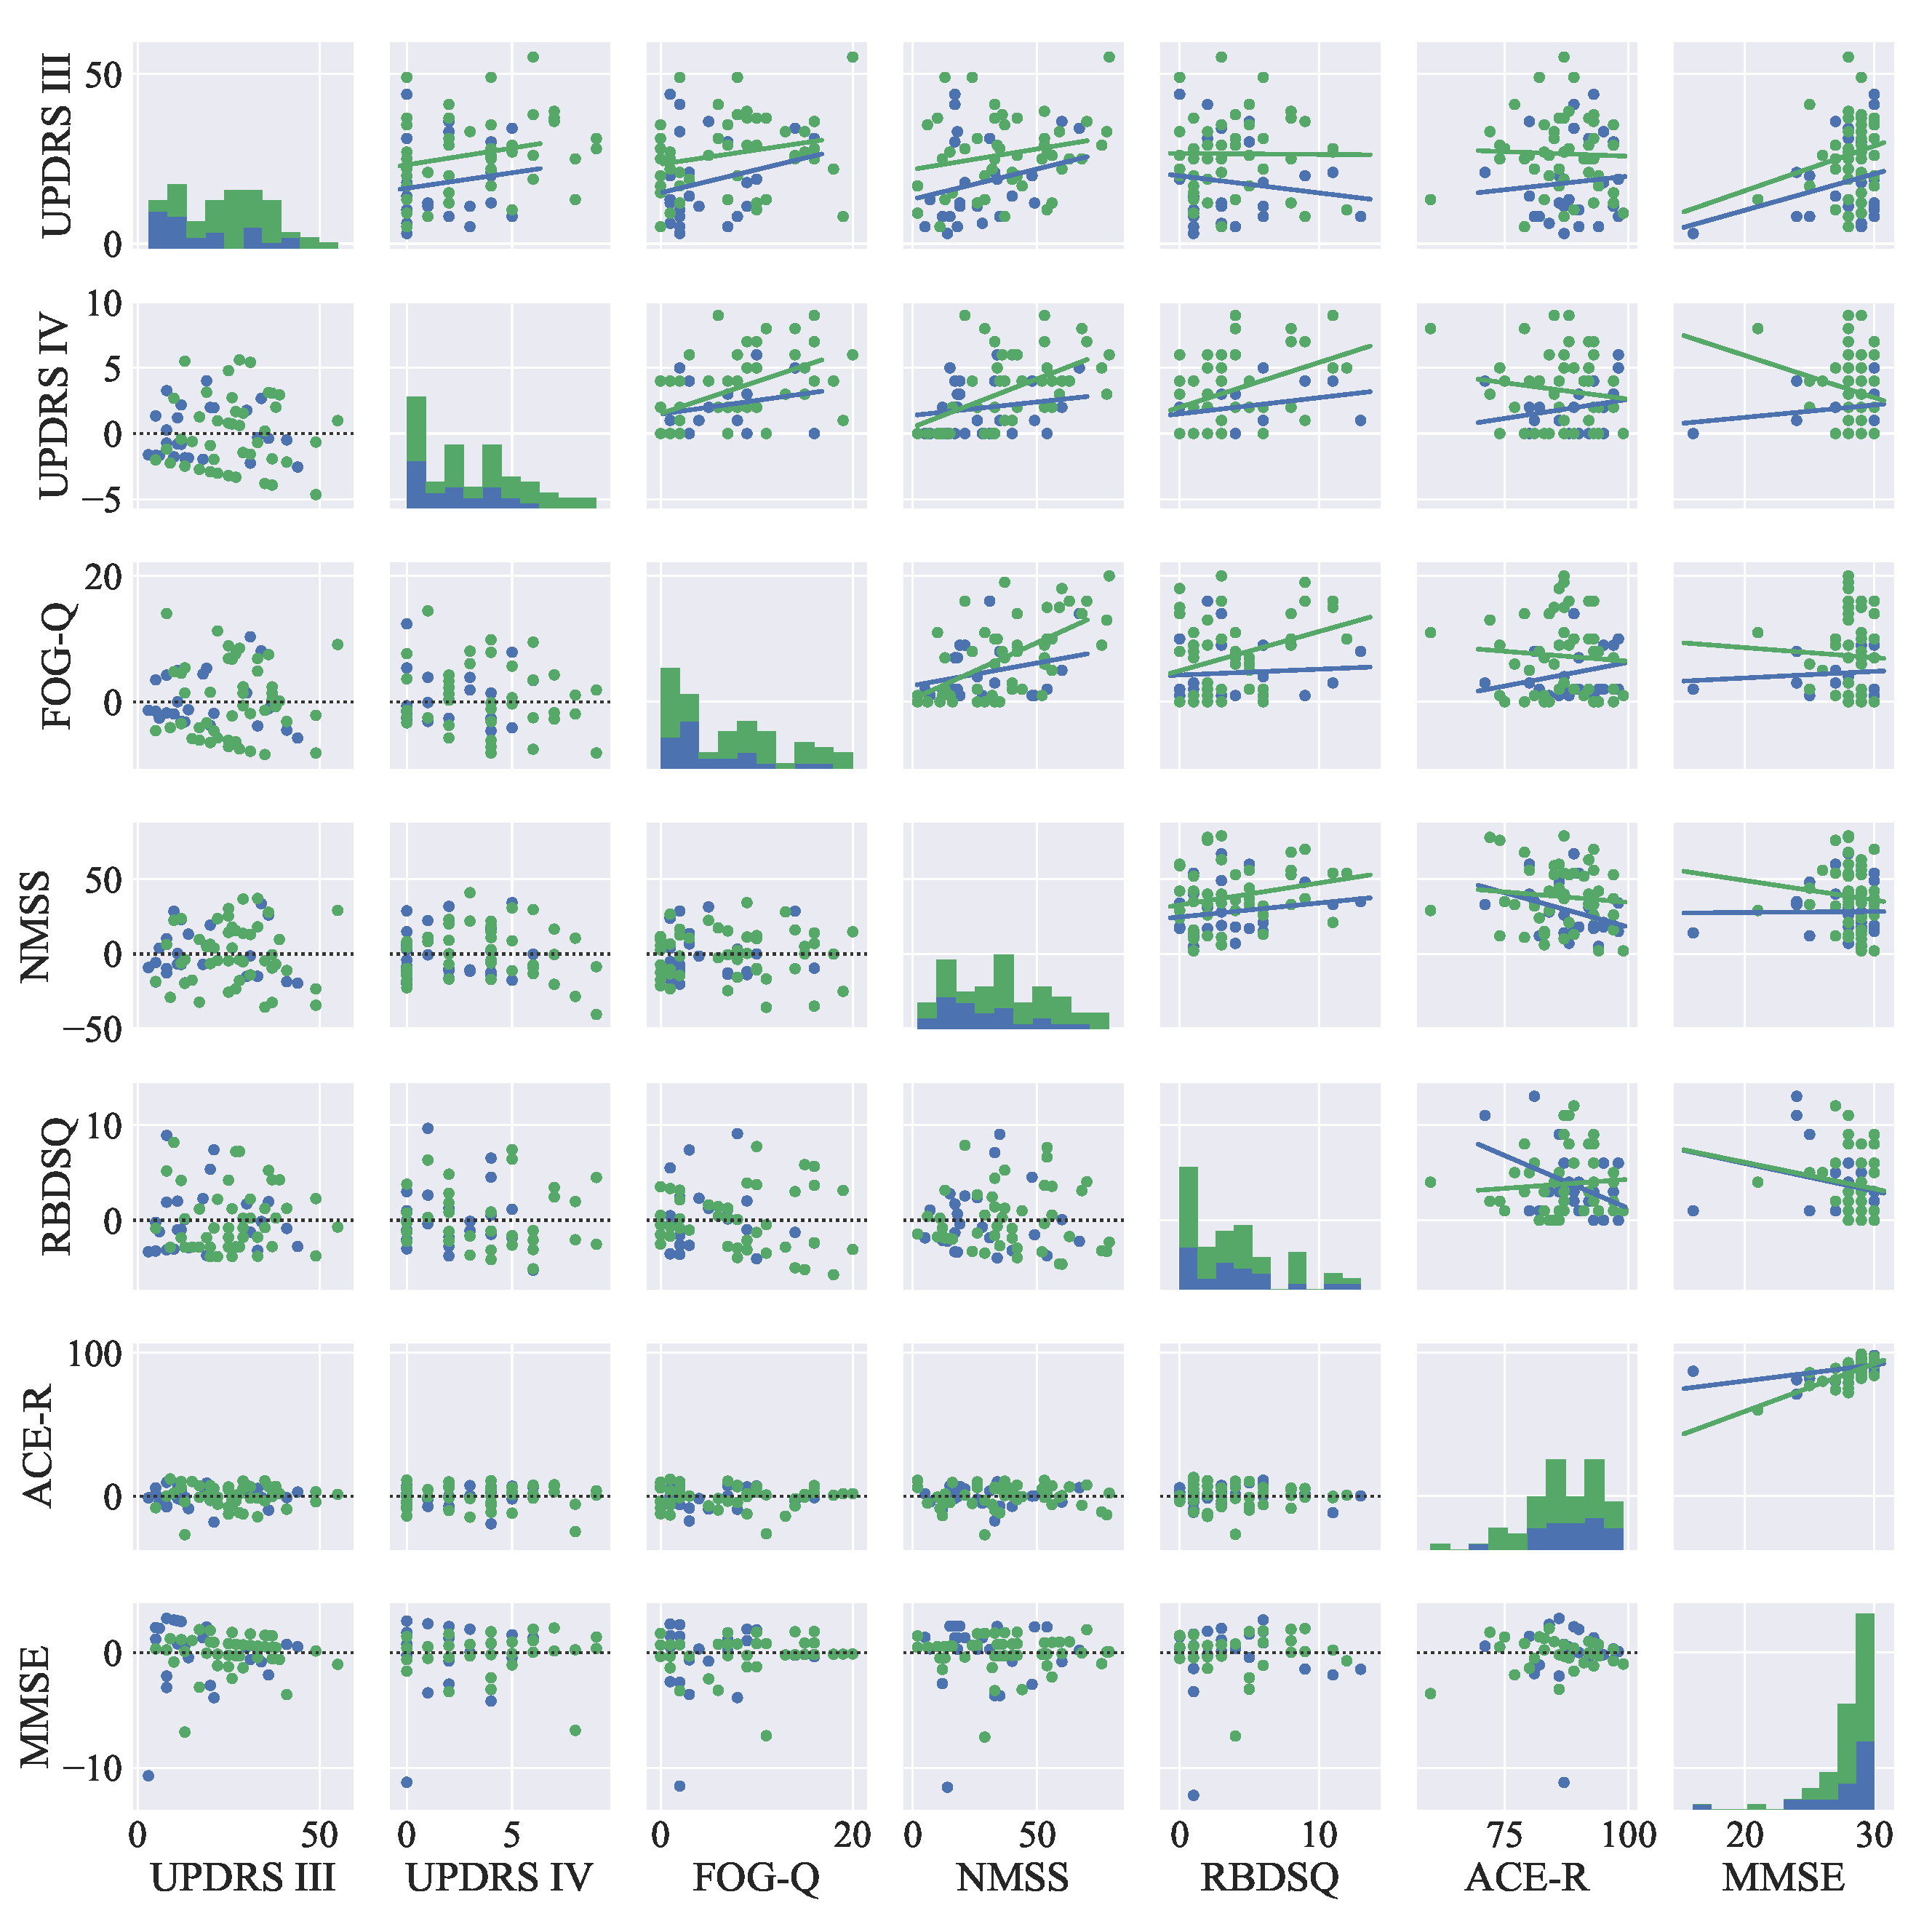
\includegraphics[width=0.99\textwidth]{pictures/ch4_clinical_statistics.eps}
	\caption[Descriptive statistical graphs of clinical data for PD patients.]{Descriptive statistical graphs of clinical characteristics (clinical rating scales) of PD patients participated in this study: on the main diagonal, histograms are visualized. Next, the upper triangular part of the graph-grid shows scatter plots along with the fitted lines of the robust linear regression models. And finally, the lower triangular part of the graph-grid is used to display residuals for the models shown in the the upper grid. Colour notation: blue colour represents female speakers, and green colour represents male speakers. For the description of the rating scales, see Table~\ref{tab:ch4_clinical_data}.}
	\label{fig:ch4_clinical_statistics}
\end{figure}

\begin{table*}[htb!]
	\centering
	\begin{threeparttable}
		\caption{Demographic and clinical characteristics of the participants.}
		\label{tab:ch4_clinical_data}
		\footnotesize
		\centering
		
		\begin{tabular}{l c c c c}
			\hline\hline\noalign{\smallskip}
			\rowcolor{gray_table}
			characteristics & PD (females) & PD (males) & HC (females) & HC (males) \\
			\noalign{\smallskip}\hline\noalign{\smallskip}

			Number of speakers  &           44         &           53         &           22         &           29         \\
			Age (years)         &   68.48~$\pm$~7.64   &   66.21~$\pm$~8.78   &   62.25~$\pm$~9.83   &   65.40~$\pm$~9.04   \\
			PD duration (years) &    7.61~$\pm$~4.85   &    7.83~$\pm$~4.39   &           -          &           -          \\
			UPDRS III           &   22.06~$\pm$~13.73  &   26.85~$\pm$~10.22  &           -          &           -          \\
			UPDRS IV            &    2.72~$\pm$~3.01   &    3.15~$\pm$~2.59   &           -          &           -          \\
			RBDSQ               &    3.42~$\pm$~3.48   &    3.85~$\pm$~2.99   &           -          &           -          \\
			FOG                 &    6.94~$\pm$~5.72   &    6.67~$\pm$~5.57   &           -          &           -          \\
			NMS                 &   36.03~$\pm$~26.72  &   38.19~$\pm$~19.72  &           -          &           -          \\
			BDI                 &   18.57~$\pm$~23.94  &    9.69~$\pm$~6.23   &           -          &           -          \\
			MMSE                &   27.38~$\pm$~3.63   &   28.56~$\pm$~1.05   &           -          &           -          \\
			LED (mg/day)        &  862.44~$\pm$~508.30 & 1087.00~$\pm$~557.47 &           -          &           -          \\
			
			\noalign{\smallskip}\hline\hline
		\end{tabular}
		
		\begin{tablenotes}
			\scriptsize
			\item Table notation: UPDRS~III\,--\,Unified Parkinson's disease rating scale, part~III: evaluation of motor function~\cite{Fahn1987}; UPDRS~IV\,--\,Unified Parkinson's disease rating scale, part~IV: evaluation of complications of therapy (Hoehn and Yahr scale, staging of severity of Parkinson's disease)~\cite{Fahn1987}; RBDSQ\,--\,The REM sleep behavior disorder screening questionnaire~\cite{Stiasny2007}; FOG-Q\,--\,Freezing of gait questionnaire~\cite{Giladi2000}; NMSS\,--\,Non-motor symptoms scale~\cite{Chaudhuri2007}; BDI\,--\,Beck depression inventory \cite{Beck2000, Beck1961}; MMSE\,--\,Mini-mental state examination~\cite{Folstein1975}; LED\,--\,L-dopa equivalent daily dose (mg/day)~\cite{Lee2010}.
		\end{tablenotes}
	\end{threeparttable}
\end{table*}

In addition to that, descriptive statistical graphs of specifically selected set of clinical characteristics for female and male speakers (only in the case of PD patients) can be seen in Figure~\ref{fig:ch4_clinical_statistics}. On the main diagonal, the graphs show histograms (i.\,e. approximation of a~distribution of the values of the clinical rating scales in the sample) for each of the rating scale. Next, on the upper triangular part of the graph-grid, scatter plots along with the lines fitted using robust linear regression can be seen. And finally, on the lower triangular part of the graph-grid, the residual plots for these models are visualized as well. With respect to the colour notation, blue colour represents female speakers and green colour represents male speakers.

Voice/speech signals were acquired by a~large capsule cardioid microphone M-AUDIO Nova~mounted to a~boom arm RODE PSA1. The microphone was positioned at a~distance of approximately $20$\,cm from the speaker's mouth. Room's environmental noise was lower than $30$\,dB sound pressure level. The signals were sampled with the sampling frequency of $48$\,kHz and consequently resampled to $16$\,kHz. All recordings were checked by a~trained acoustic engineer who discarded those, which contain some undesirable noise (such as speech therapist's cough, phone ringing, etc.). All the participants signed an informed consent form that had been approved by the Ethics Committee of St. Anne's University Hospital in Brno.

With respect to the speech tasks used to quantify prosodic deterioration in HD, the following three speech task scenarios comprising two reading tasks and a~poem recitation task were considered. First of all, every participant performed two reading tasks ($1$. emotionally-neutral reading, and $2$. stress-modified reading). Next, all speakers were asked to recite a~poem composed of two rhymes. At first, they were instructed to read the poem on a~paper. After that, every participant recited this poem into a~microphone, but without any need to keep it in memory (i.\,e. no memory-related constraints were applied). The tasks:
\begin{enumerate}

	\item Reading~a short paragraph with neutral emotion. 
	In Czech (original)\,--\,\textit{I na tom, \v{z}e \v{c}lov\v{e}k si opat\v{r}\'{i} psa, aby nebyl s\'{a}m, je mnoho pravdy. Pes opravdu nechce b\'{y}t s\'{a}m.}; In English\,--\,\textit{Even the fact that a~man gets a~dog to not be alone is pretty much true. A~dog really don't want to be alone.}

	\item Stress-modified reading. 
	In Czech (original)\,--\,\textit{Te\v{d} mus\'{i}\v{s} b\'{y}t chv\'{i}li trp\v{e}liv\'{y}, ne\v{z} to dokon\v{c}\textbf{}me. U\v{z} m\v{e} to nebav\'{i}, dej mi u\v{z} kone\v{c}n\v{e} pokoj! Tak co, jak to dopadlo?}; In English\,--\,\textit{Now, you have to be patient until we finish it. I'm tired of it already, leave me alone! So, how did it go?}

	\item Poem recitation task. 
	In Czech (original)\,--\,\textit{Chcete vid\v{e}t velk\'{y} lov? Budu lovit v d\v{z}ungli slov. Osedl\'{a}m si Pegasa, chyt\'{\i}m b\'{a}se\v{n} do lasa!}, ; In English\,--\,\textit{Would you like to see a~big hunt? I will be hunting in a~jungle of words. I will saddle the Pegasus, I will catch a~poem into a~lasso.}
\end{enumerate}

\subsection{Feature extraction}
\label{ch4_3_2}

To describe dysprosody in HD, several conventional and clinically well-interpretable acoustic features~\cite{Brabenec2017} were used. The following acoustic features quantifying a~relative variability of speech intonation were computed: standard deviation of F0\footnote{In the case of pitch variation, fundamental frequency (F0) was used~\cite{Boersma2012}.} (FOSD); relative standard deviation\footnote{Standard deviation divided by the mean of the variable.} of F0 (relF0SD); variation range\footnote{Difference between minimum and maximum value of the variable.} of F0 (FOVR); and relative variation range\footnote{Variation range divided by the mean of the variable.} of F0 (relF0VR). In the case of intensity variation, squared energy operator (SEO) and Teager-Kaiser energy operator (TEO) were computed to quantify the intensity of voice/speech signals. The following acoustic features quantifying a~relative variability of speech intensity were computed: standard deviation of SEO/TEO (SEOSD/TEOSD); relative standard deviation of SEO/TEO (relSEOSD/relTEOSD); variation range of SEO/TEO (SEOVR/TEOVR); and relative variation range of SEO/TEO (relSEOVR/relTEOVR). Next, several features describing speech rate and pausing abnormalities in HD, such as total speech time (TST), net speech time (NST), total pause time (TPT), total speech rate (TSR), net speech rate (NSR), total pause time (pauses longer than $50$\,ms) (TPT\,($50$\,ms)), articulation rate (AR), and speech index of rhythmicity (SPIR) were computed. For more information about these features, see Appendix~\ref{tab:prosodic_features}, and the review article focused on the acoustic analysis in patients with PD~\cite{Brabenec2017}.

\subsection{Analytical setup}
\label{ch4_3_3}

To obtain an insight into the statistical properties of the acoustic features used to quantify dysprosody in HD, the approach of Tsanas et al.~\cite{Tsanas2010} using Spearman's correlation coefficient ($\rho$) and mutual information (MI) between the features and the associated clinical diagnosis (HC/PD) was followed. Spearman's correlation coefficient is a~statistical measure of the strength of a~monotonic relationship between feature vectors and the associated response variable~\cite{Sheskin2007}. Mutual information is a~measure of the amount of the information shared by two random variables (the larger the value of MI, the stronger statistical association between feature and the response can be observed). MI is defined as follows:
\begin{equation}
	I(X; Y) = \int_X\int_Y f(x, y) \log_2 \left(\frac{f(x, y)}{f_X(x)f_Y(y)} \right),
\end{equation}
where $X$ and $Y$ are both random variables with the associated joint probability density function $f(x, y)$, and marginal density functions $f_X(x)$ and $f_Y(y)$, respectively. For the purpose of this study, marginal entropies $H(X)$ and $H(Y)$, and joint entropy $H(X,Y)$ were used to compute MI. With this approach, MI is defined as:
\begin{equation}
	I(X; Y) = H(X) + H(Y) - H(X, Y).
\end{equation}

Moreover, Mann-Whitney U~test was used to compare the distribution of the prosodic features between HC and patients with PD. The Mann-Whitney U~test is a~non-parametric statistical test that is used to assess whether two independent groups of variables are significantly different from each other~\cite{Birnbaum1956}. It is defined as:
\begin{equation}
	U = R_1 - \frac{n_1 (n_1 + 1)}{2},
\end{equation}
where $n_1$ is the sample size for sample $1$, and $R_1$ is the sum of the ranks in sample $1$. Note that it is not specified which sample is considered sample $1$, and therefore and equally valid statement can be made using sample $2$ ($n_2$ instead of $n_1$ and $R_2$ instead of $R_1$, respectively).

To evaluate an individual power of each of the acoustic features to discriminate healthy and dysarthric speech, every feature was used separately as an input to the random forest (RF) classifier (univariate models). Random forest is an ensemble learning algorithm operating by constructing a~multiple of base learners~\cite{Breiman2001} that are used for classifying new samples via voting mechanism. To optimise the trained models, grid-search technique over the set of tunable parameters was performed: the number of features over which RF performs a~search while constructing each branch was selected to be equal to the square root of the number of input features; and the maximum number of $500$ trees was chosen for this classifier.

Next, to build models capable of HD discrimination based on the combination of acoustic features, i.\,e. combination of the prosodic impairments present in HD, multivariate models were trained as well. For this purpose, RF classifier with the same tuning parameters as in the case of univariate models was used. However, to select only the relevant set of features and to build clinically interpretable models with low dimensionality (prediction models with less features are in general less prone overfitting), a~feature selection process was applied~\cite{Guyon2006}. For this purpose, a~modified version of sequential floating forward selection (SFFS) algorithm proposed by Pohjalainen et al.~\cite{Pohjalainen2014} in $2014$ was used.

To quantify the classification performance of the models, Matthew's correlation coefficient~\cite{Matthews1975} (MCC) as a~reference performance measurement employed on unbalanced data sets~\cite{Jurman2012}, accuracy (ACC), sensitivity (SEN), and specificity (SPE)\footnote{In the frame of this study, ACC, SEN, and SPE are are expressed in $\%$, and therefore should be rather referred to as: $P_\mathrm{ACC}$, $P_\mathrm{SEN}$, $P_\mathrm{SPE}$ as the ACC, SEN, and SPE are expressed as rational numbers. However, for the simplicity and easier interpretability of the results, classical abbreviations (ACC, SEN, SPE) are used.} were computed. MCC was also used as a~ measure assessing the classification performance of the models during a~feature selection process. All metrics however are useful when used to describe properties of the build models (described bellow). The metrics are defined as:
\begin{eqnarray}
	\mathrm{MCC} &=& \frac{TP \times TN + FP \times FN}{\sqrt{N}}, \\
	\mathrm{ACC} &=& \frac{TP + TN}{M} \cdot 100\,[\%], \\
	\mathrm{SEN} &=& \frac{TP}{TP + FN} \cdot 100\,[\%], \\
	\mathrm{SPE} &=& \frac{TN}{TN + FP} \cdot 100\,[\%],
\end{eqnarray}
where the variables denote: $N = (TP + FP)(TP + FN)(TN + FP)(TN + FN)$, $M = TP + TN + FP + FN$. $TP$ (true positive) and $FP$ (false positive) represents the number of correctly identified PD subjects and a~number of subjects identified as PD, but being healthy. Similarly, $TN$ (true negative) and $FN$ (false negative) represent the total number of correctly identified healthy controls, and PD patients identified as HC. In the frame of this study, these classification metrics can be interpreted as: accuracy expresses the proportion of correctly identified PD patients as well as healthy subjects ($TP + TN$) out of all subjects ($TP + TN + FP + FN$), so that with higher accuracy, fewer miss-classifications are made; sensitivity expresses the proportion of participants correctly identified as having PD ($TP$) out of all patients with PD ($TP + FN$), so that with higher sensitivity, fewer actual cases of PD go undetected; and specificity expresses the proportion of participants correctly identified not as having PD ($TN$) out of all healthy subjects ($TN + FP$), so that with higher specificity, fewer healthy subjects are labelled as having PD.

The theoretical chance level of binary classification is $50$\,\%. This threshold is based on the assumption of infinite sample size, which does not hold in practice. The empirical chance level depends on the actual number of samples in the used dataset and therefore it is common to see the empirical chance level noticeably above the theoretical threshold for small datasets ($60$\% or even higher)~\cite{Combrisson2015}. As the sample size grows, the empirical chance level is getting closer to its theoretical value. With the growing dimension of feature space required sample size grows exponentially. So, to find out if the classification results were obtained by chance or by the actual relationship between the class labels and the data a~non-parametric statistical method: permutation test was used. Permutation test is commonly used tool in biostatistical research. It makes no particular assumptions about statistical properties of the samples except that the observations are independent and identically distributed under the null hypothesis, which makes it highly attractive~\cite{Phipson2010}. The main idea behind permutation tests used in classifier performance evaluation is the following: The null hypothesis is that the observations are independently and identically distributed (in other words, there is no relation between the class labels and the data). The alternative hypothesis is that the distribution differs between groups (in our case between PD and HC groups). The null hypothesis testing requires the p-value to be determined. The most commonly used approach is to estimate the p-value by randomly permuting the labels to obtain the empirical null distribution~\cite{Phipson2010}, however, in the frame of this study, the exact p-value is used to mitigate the type~I error rate and the multiple testing issues~\cite{Phipson2010}.

Thus, if the computed p-value is bellow a~chosen significance level $\alpha$ then the null hypothesis can be rejected. In this study, the $\alpha$ of $0.01$ was selected. Tested classification models with p-values bellow $\alpha$ were consider sufficiently high above chance level. Matthew's correlation coefficient was chosen as a~test statistic for the permutation test as it is the measure used to assess the classification performance of the models during a~feature selection step. The number of permutations was selected to be equal to $1000$ and the classifier validation was conducted using stratified $10$-fold cross-validation with $20$ repetitions~\cite{Ojala2009, Combrisson2015}.

\section{Results}
\label{ch4_4}

Results of the univariate analysis are summarized in Table~\ref{tab:ch4_statistical_analysis}. As can be seen, the best classification performance in terms of the classification accuracy computed for the univariate models can be summarized as follows: a) poem recitation task\,--\,$\mbox{ACC}=64.2\,\%$ (female participants), $\mbox{ACC}=64.6\,\%$ (male participants), and $\mbox{ACC}=68.5\,\%$ (all participants); b) reading with neutral emotion\,--\,$\mbox{ACC}=62.7\,\%$ (female participants), $\mbox{ACC}=69.1\,\%$ (male participants), and $\mbox{ACC}=58.4\,\%$ (all participants); and c) stress-modified reading\,--\,$\mbox{ACC}=68.7\,\%$ (female participants), $\mbox{ACC}=67.1\,\%$ (male participants), and $\mbox{ACC}=59.7\,\%$ (all participants).

\begin{table*}[tb!]
	\centering
	\begin{threeparttable}
		\caption{Statistical analysis of the prosodic features.}
		\label{tab:ch4_statistical_analysis}
		\footnotesize
		\centering
		\begin{tabular}{l l l r c c c c c} 
		
		\hline\hline\noalign{\smallskip}
		\rowcolor{gray_table}
		gender & features & disorder & $\rho$ & MI & $p$ & ACC & SEN & SPE \\
		\noalign{\smallskip}
		& \multicolumn{6}{c}{Poem recitation task} \\
		\noalign{\smallskip}\hline\noalign{\smallskip}

			\multirow{3}{*}{females}
			& relSEOSD & monoloudness &  0.10 & 0.97 &    & 64.2 & 72.5 & 51.9 \\
			& NST      & speech rate  & -0.23 & 0.88 &    & 62.7 & 67.5 & 55.6 \\
			& NSR      & speech rate  &  0.23 & 0.88 &    & 61.2 & 65.0 & 55.6 \\
			\noalign{\smallskip}

			\multirow{3}{*}{males}
			& F0VR     & monopitch    & -0.12 & 0.90 &    & 64.6 & 64.3 & 65.4 \\
			& TEOVR    & monoloudness & -0.18 & 0.90 &    & 62.2 & 62.5 & 61.5 \\
			& rellF0SD & monopitch    & -0.21 & 0.90 &    & 61.0 & 67.9 & 46.2 \\
			\noalign{\smallskip}

			\multirow{3}{*}{all} 
			& TPT & speech rate & -0.17 & 0.94 & *  & 68.5 & 70.8 & 64.2 \\
			& NST & speech rate & -0.11 & 0.79 &    & 63.1 & 69.8 & 50.9 \\
			& NSR & speech rate &  0.11 & 0.79 &    & 61.8 & 69.8 & 47.2 \\

		\noalign{\smallskip}\hline\noalign{\smallskip}
		& \multicolumn{6}{c}{Reading with neutral emotion} \\
		\noalign{\smallskip}\hline\noalign{\smallskip}
			
			\multirow{3}{*}{females}
			& F0VR          & monopitch   & -0.07 & 0.97 &    & 62.7 & 67.5 & 55.6 \\
			& TPT\,(50\,ms) & speech rate &  0.05 & 0.94 &    & 61.2 & 60.0 & 63.1 \\
			& AR            & speech rate & -0.05 & 0.94 &    & 61.2 & 60.0 & 63.0 \\
			\noalign{\smallskip}

			\multirow{3}{*}{males}
			& relSEOVR & monoloudness & -0.06 & 0.90 &    & 64.6 & 71.4 & 50.0 \\
			& relTEOSD & monoloudness &  0.27 & 0.90 & *  & 62.2 & 64.3 & 57.7 \\
			& relTEOVR & monoloudness &  0.28 & 0.90 & ** & 61.1 & 66.1 & 50.0 \\
			\noalign{\smallskip}

			\multirow{3}{*}{all}
			& relSEOSD      & monoloudness &  0.04 & 0.94 &    & 58.4 & 60.4 & 54.7 \\
			& relSEOVR      & monoloudness & -0.01 & 0.94 &    & 57.7 & 60.4 & 52.8 \\
			& TPT\,(50\,ms) & speech rate  &  0.03 & 0.82 &    & 54.4 & 58.3 & 47.2 \\
			
		\noalign{\smallskip}\hline\noalign{\smallskip}			
		& \multicolumn{6}{c}{Stress-modified reading task} \\
		\noalign{\smallskip}\hline\noalign{\smallskip}
			
			\multirow{3}{*}{females}
			& relTEOVR & monoloudness & -0.36 & 0.97 & ** & 68.7 & 70.0 & 66.7 \\
			& F0SD     & monopitch    & -0.22 & 0.97 &    & 64.2 & 65.0 & 63.0 \\
			& relTEOSD & monoloudness & -0.38 & 0.97 & ** & 59.7 & 55.0 & 66.7 \\
			\noalign{\smallskip}

			\multirow{3}{*}{males}
			& TPT\,(50\,ms) & speech rate  & -0.29 & 0.83 & *  & 67.1 & 71.4 & 57.7 \\
			& AR            & speech rate  &  0.29 & 0.83 & *  & 67.1 & 71.4 & 57.7 \\
			& relTEOVR      & monoloudness &  0.03 & 0.90 &    & 59.8 & 67.9 & 42.3 \\
			\noalign{\smallskip}

			\multirow{3}{*}{all}
			& TPT   & speech rate  & -0.26 & 0.93 & ** & 59.7 & 65.6 & 49.1 \\
			& F0SD  & monopitch    & -0.26 & 0.94 & ** & 57.8 & 61.5 & 51.0 \\
			& TEOVR & monoloudness & -0.15 & 0.94 &    & 57.7 & 62.5 & 49.1 \\
			
			\noalign{\smallskip}\hline\hline
		\end{tabular}
		
		\begin{tablenotes}
			\scriptsize
			\item Table notation: $\rho$\,--\,Spearman's rank correlation coefficient; MI\,--\,mutual information; $p$\,--\,p-values of Mann-Whitney U test (* means $p<0.05$; ** means $p<0.01$); ACC\,--\,classification accuracy; SEN\,--\,classification sensitivity; SPE\,--\,classification specificity. ACC, SEN, SPE: expressed in $\%$.
		\end{tablenotes}
	\end{threeparttable}
\end{table*}

Regarding the Mann-Whitney U~test, there are few statistically significant differences, specifically: a) poem recitation task\,--\,$p<0.01$ for TPT (all participants); b) reading with neutral emotion\,--\,$p<0.05$ for relTEOSD (males), and $p<0.01$ for relTEOVR (males); and c) stress-modified reading\,--\,$p<0.05$ for TPT\,(50\,ms) (males), AR (males), and $p<0.01$ for relTEOVR (females), relTEOSD (females), TPT (all participants), and F0SD (all participants). Next, a~comparison of the features expressing monopitch (F0SD), monoloudness (SEOSD), and speech rate abnormalities (NSR) between PD patients and HC can be seen in Table~\ref{tab:ch4_comparisons} and Figures~\ref{fig:ch4_comparisons_females},~\ref{fig:ch4_comparisons_males}, and~\ref{fig:ch4_comparisons_all}.

\begin{table}[!htb]
	\centering
	\begin{threeparttable}
		\caption{Comparison of acoustic features between PD speakers and HC.}
		\label{tab:ch4_comparisons}
		\footnotesize
		\centering
		\begin{tabular}{l l l c c c} 

			\hline\hline\noalign{\smallskip}
			\rowcolor{gray_table}
			gender & features & disorder & PD & HC & diff [\%] \\
			\noalign{\smallskip}
			\multicolumn{6}{c}{Poem recitation} \\
			\noalign{\smallskip}\hline\noalign{\smallskip}
			
			\multirow{3}{*}{females} &
			  F0SD  & monopitch    & 101.87~$\pm$~8.01 & 107.42~$\pm$~8.91 & PD < HC (5.17) \\
			& SEOSD & monoloudness &   6.30~$\pm$~3.67 &   5.61~$\pm$~3.17 & PD > HC (12.30) \\
			& NSR 	& speech rate  &  15.53~$\pm$~2.66 &  19.24~$\pm$~17.94 & PD < HC (19.28) \\
			\noalign{\smallskip}
			
			\multirow{3}{*}{males} &
			  F0SD  & monopitch    &  75.55~$\pm$~14.06 &  80.90~$\pm$~11.18 & PD < HC (6.61) \\
			& SEOSD & monoloudness &   6.44~$\pm$~3.48  &   7.02~$\pm$~3.67 & PD < HC (8.26) \\
			& NSR 	& speech rate  &  18.09~$\pm$~12.71 &  16.14~$\pm$~2.95 & PD > HC (17.10) \\
			\noalign{\smallskip}
			
			\multirow{3}{*}{all} &
			  F0SD  & monopitch    &  86.49~$\pm$~17.60 &  94.06~$\pm$~16.64 & PD < HC (8.05) \\
			& SEOSD & monoloudness &   6.42~$\pm$~3.54  &   6.28~$\pm$~3.48 & PD > HC (2.23) \\
			& NSR 	& speech rate  &  17.00~$\pm$~9.82  &  17.65~$\pm$~12.71 & PD < HC (3.68) \\
			
			\noalign{\smallskip}\hline\noalign{\smallskip}
			\multicolumn{6}{c}{Reading with neutral emotion} \\
			\noalign{\smallskip}\hline\noalign{\smallskip}				
			
			\multirow{3}{*}{females} &
			  F0SD  & monopitch    &  93.69~$\pm$~8.58  &  98.27~$\pm$~7.58 & PD < HC (4.66) \\
			& SEOSD & monoloudness &   5.97~$\pm$~3.37  &   6.03~$\pm$~2.67 & PD < HC (1.00) \\
			& NSR 	& speech rate  &  14.24~$\pm$~4.78  &  13.91~$\pm$~4.59 & PD > HC (2.37) \\
			\noalign{\smallskip}
			
			\multirow{3}{*}{males} &
			  F0SD  & monopitch    &  71.81~$\pm$~12.36 &  70.51~$\pm$~11.33 & PD > HC (1.84) \\
			& SEOSD & monoloudness &   6.67~$\pm$~3.03  &   5.42~$\pm$~2.15 & PD > HC (23.06) \\
			& NSR 	& speech rate  &  13.49~$\pm$~3.29  &  12.86~$\pm$~1.86 & PD > HC (4.90) \\
			\noalign{\smallskip}
			
			\multirow{3}{*}{all} &
			  F0SD  & monopitch    &  80.86~$\pm$~15.40 &  84.26~$\pm$~16.90 & PD < HC (4.04) \\
			& SEOSD & monoloudness &   6.39~$\pm$~3.16  &   5.68~$\pm$~2.42 & PD > HC (12.50) \\
			& NSR 	& speech rate  &  13.77~$\pm$~3.97  &  13.42~$\pm$~3.46 & PD > HC (2.61) \\
			
			\noalign{\smallskip}\hline\noalign{\smallskip}
			\multicolumn{6}{c}{Stress-modified reading} \\
			\noalign{\smallskip}\hline\noalign{\smallskip}

			\multirow{3}{*}{females} &
			  F0SD  & monopitch    &  91.27~$\pm$~11.13 &  95.72~$\pm$~6.71 & PD < HC (4.65) \\
			& SEOSD & monoloudness &   5.57~$\pm$~2.71  &   5.55~$\pm$~2.53 & PD > HC (0.36) \\
			& NSR 	& speech rate  &  17.20~$\pm$~3.22  &  19.44~$\pm$~12.40 & PD < HC (11.52) \\
			\noalign{\smallskip}

			\multirow{3}{*}{males} &
			  F0SD  & monopitch    &  68.87~$\pm$~10.11 &  74.86~$\pm$~13.44 & PD < HC (8.00) \\
			& SEOSD & monoloudness &   6.53~$\pm$~3.27  &   5.57~$\pm$~2.62 & PD > HC (17.24) \\
			& NSR 	& speech rate  &  19.35~$\pm$~8.95  &  18.37~$\pm$~4.45 & PD > HC (5.33) \\
			\noalign{\smallskip}
			
			\multirow{3}{*}{all} &
			  F0SD  & monopitch    &  78.05~$\pm$~15.42 &  85.50~$\pm$~14.44 & PD < HC (8.71) \\
			& SEOSD & monoloudness &   6.16~$\pm$~3.07  &   5.48~$\pm$~2.52 & PD > HC (12.41) \\
			& NSR 	& speech rate  &  18.49~$\pm$~7.15  &  18.82~$\pm$~9.17 & PD < HC (1.75) \\

			\noalign{\smallskip}\hline\hline
		\end{tabular}
		
		\begin{tablenotes}
			\scriptsize
			\item Table notation: diff [\%]\,--\,difference between the mean values for patients with PD and HC. All prosodic features for PD patients and HC are represented as mean~$\pm$~sd.
		\end{tablenotes}
	\end{threeparttable}
\end{table}

\newpage
From the perspective of the monopitch, reduced variation in F0 can be observed in $8$ out of the total number of $9$ scenarios. The only exception occurs in the case of male speakers reading a~passage with neutral emotion, which in general does not require that much variation in speech intonation or stress, so that this particular deviation is quiet acceptable. Regarding the monoloudness, interestingly there are $7$ cases in which PD patients show more variation in speech intensity than HC, which is in contradiction with the original assumption of lowered variation in speech intensity in patients with PD in comparison with HC. The only two exceptions lies in the neutral reading task, and the poem recitation task performed by male speakers. However, in contrast to that, female patients did show significantly lower speech intensity when compared to HC while performing the poem recitation. Thus, the results suggest a~presence of a~gender-related pattern of parkinsonian speech intensity variation and control deterioration. Finally, in the case of speech rate abnormalities, PD patients seem to have lower speech rate that HC when performing a~task that requires stress (stress-modified reading) or changes in the melody of speech (poem recitation). In the case of male participants, PD patients seem to have higher speech rate when compared to HC. And finally, in the case of female participants, the same phenomenon can be observed when the data for both genders are merged together.

\begin{figure}[htb!]
	\centering
	\scriptsize
	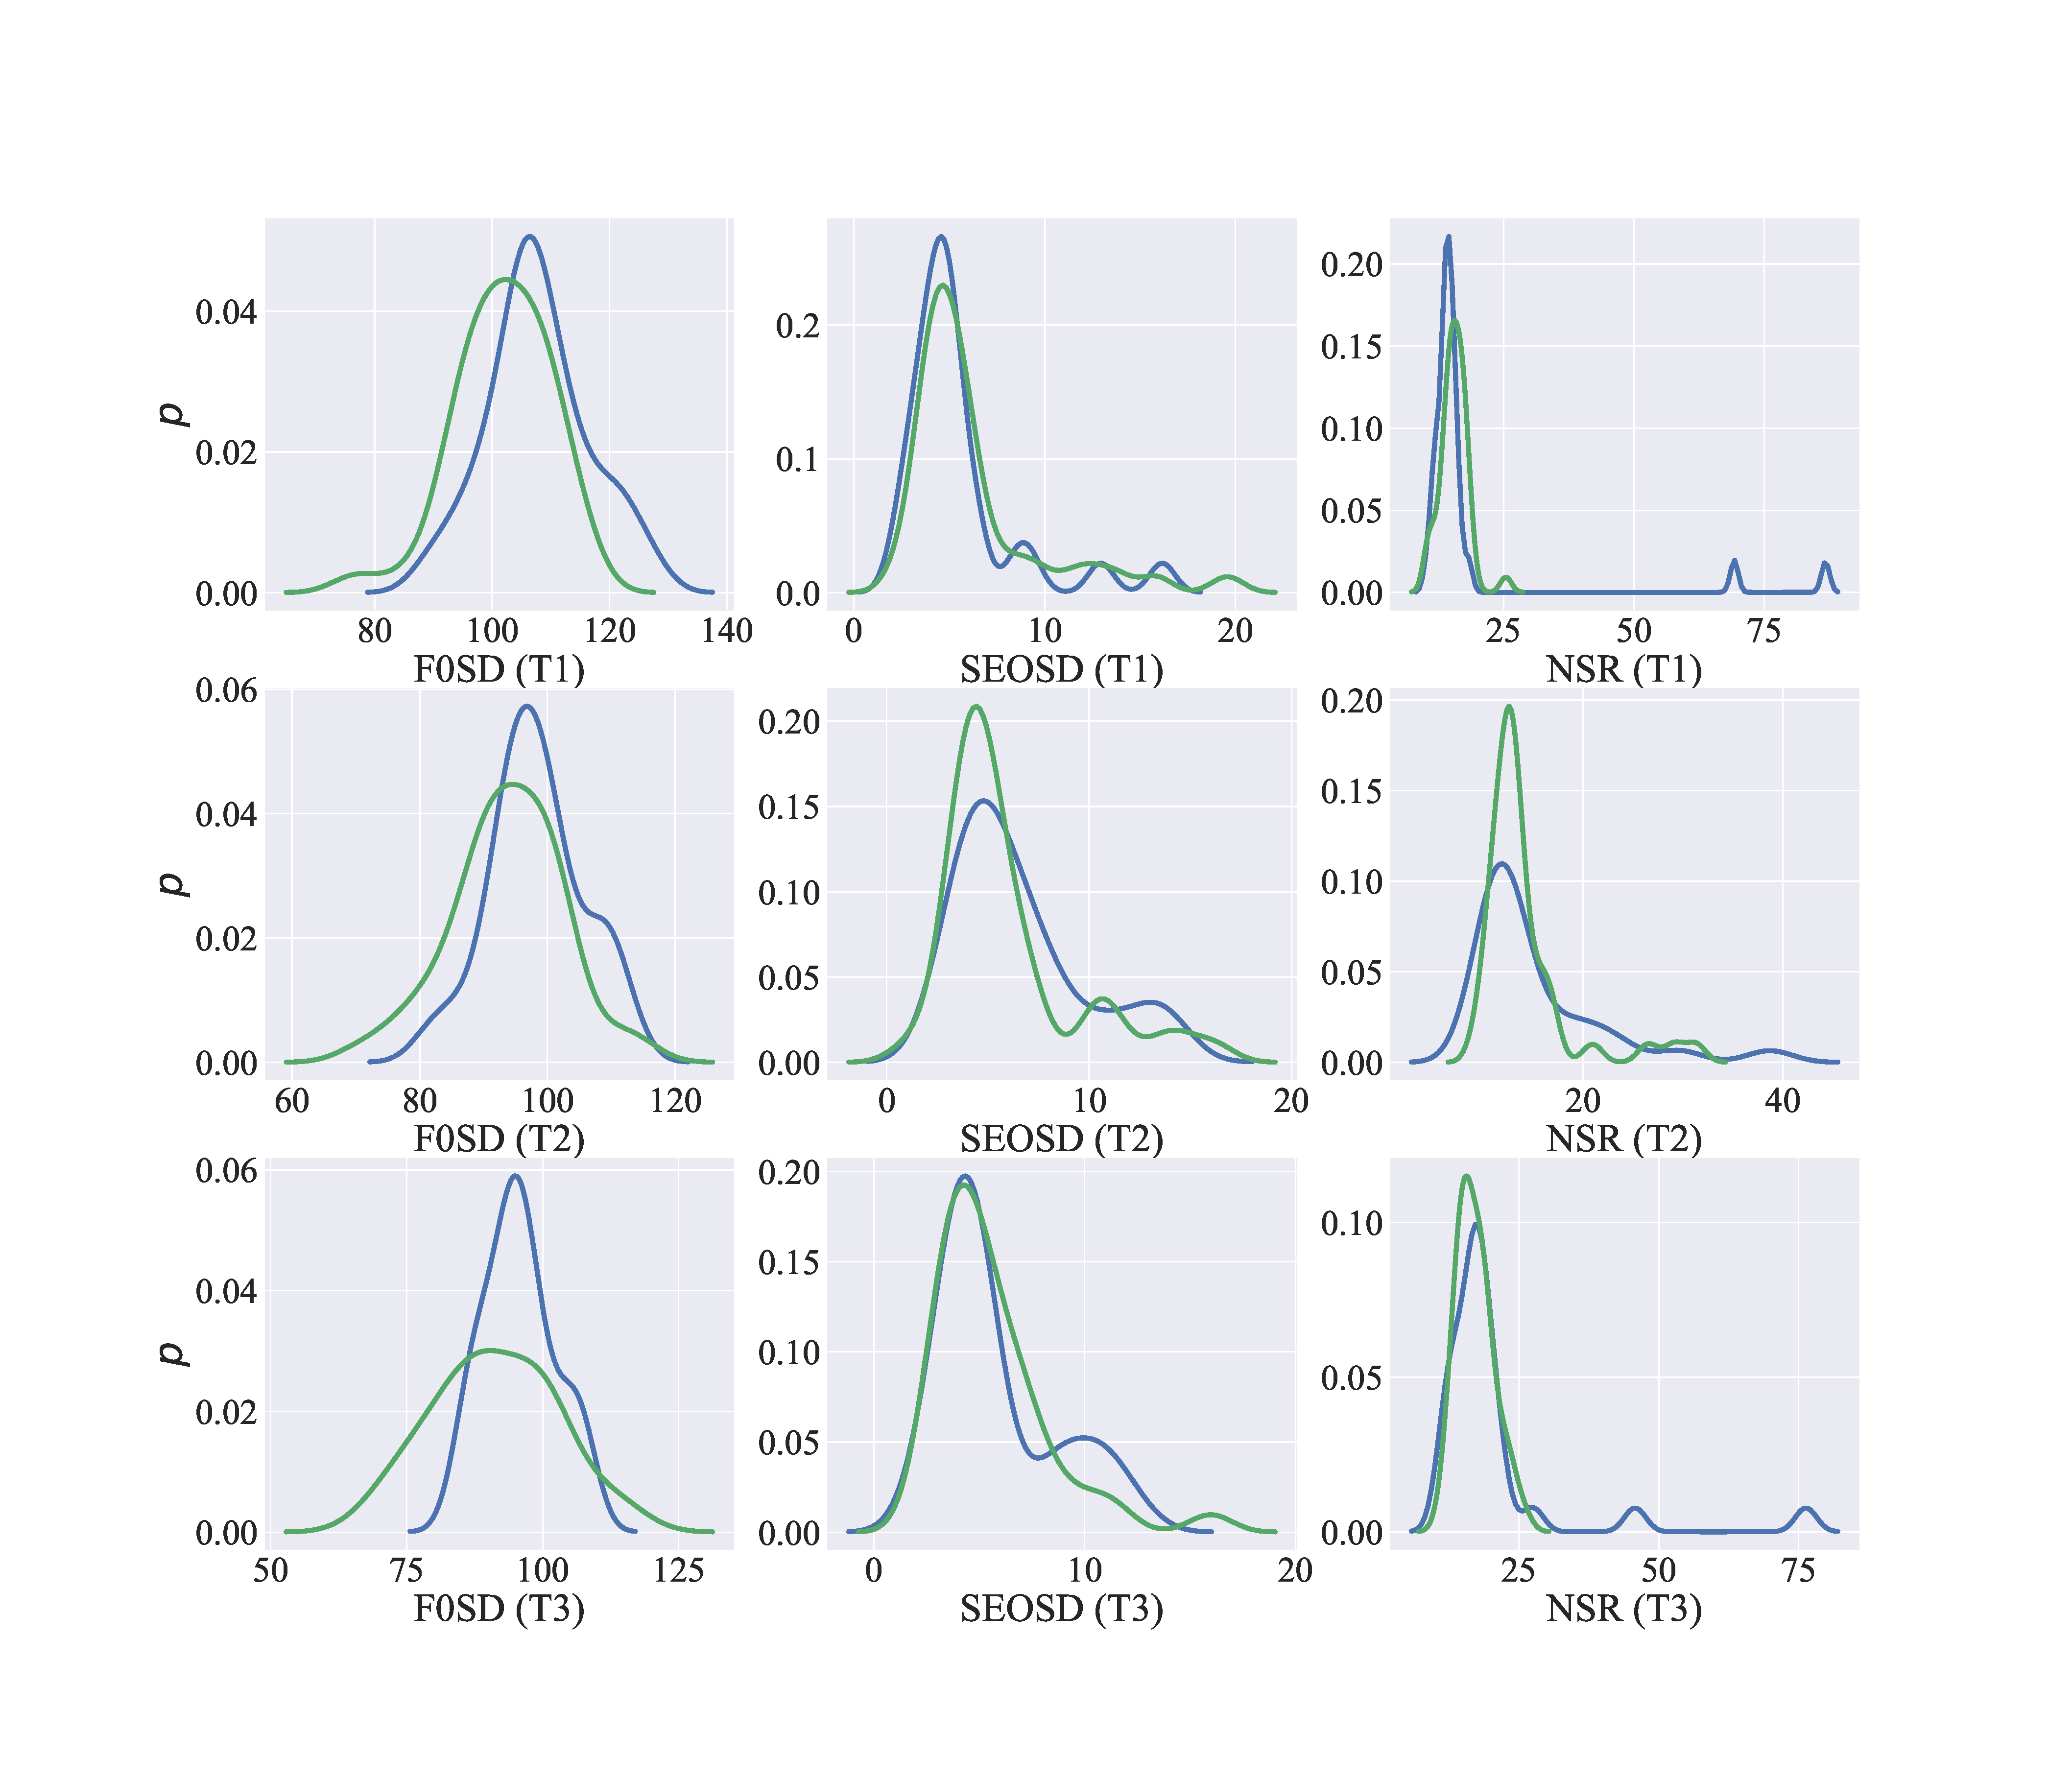
\includegraphics[width=0.99\textwidth]{pictures/ch4_comparisons_females.eps}
	\caption[Density estimation plots for female speakers.]{Density estimation plots (computed using kernel probability density estimation with Gaussian kernels) for selected acoustic features for all three speech tasks performed by female speakers only: T1\,--\,poem recitation task (first row); T2\,--\,emotionally-neutral reading (second row); and T3\,--\,stress-modified reading (third row). Colour notation: blue colour represents healthy speakers, and green colour represents speakers with PD. Feature notation: F0SD (standard deviation of fundamental frequency) expresses variability of intonation (melody of speech); SEOSD (standard deviation of squared energy operator) expresses variability of speech intensity (melody of speech); and NSR (net speech rate) expresses the number of phones per entire duration of speech without pauses (speech rate).}
	\label{fig:ch4_comparisons_females}
\end{figure}

\begin{figure}[htb!]
	\centering
	\scriptsize
	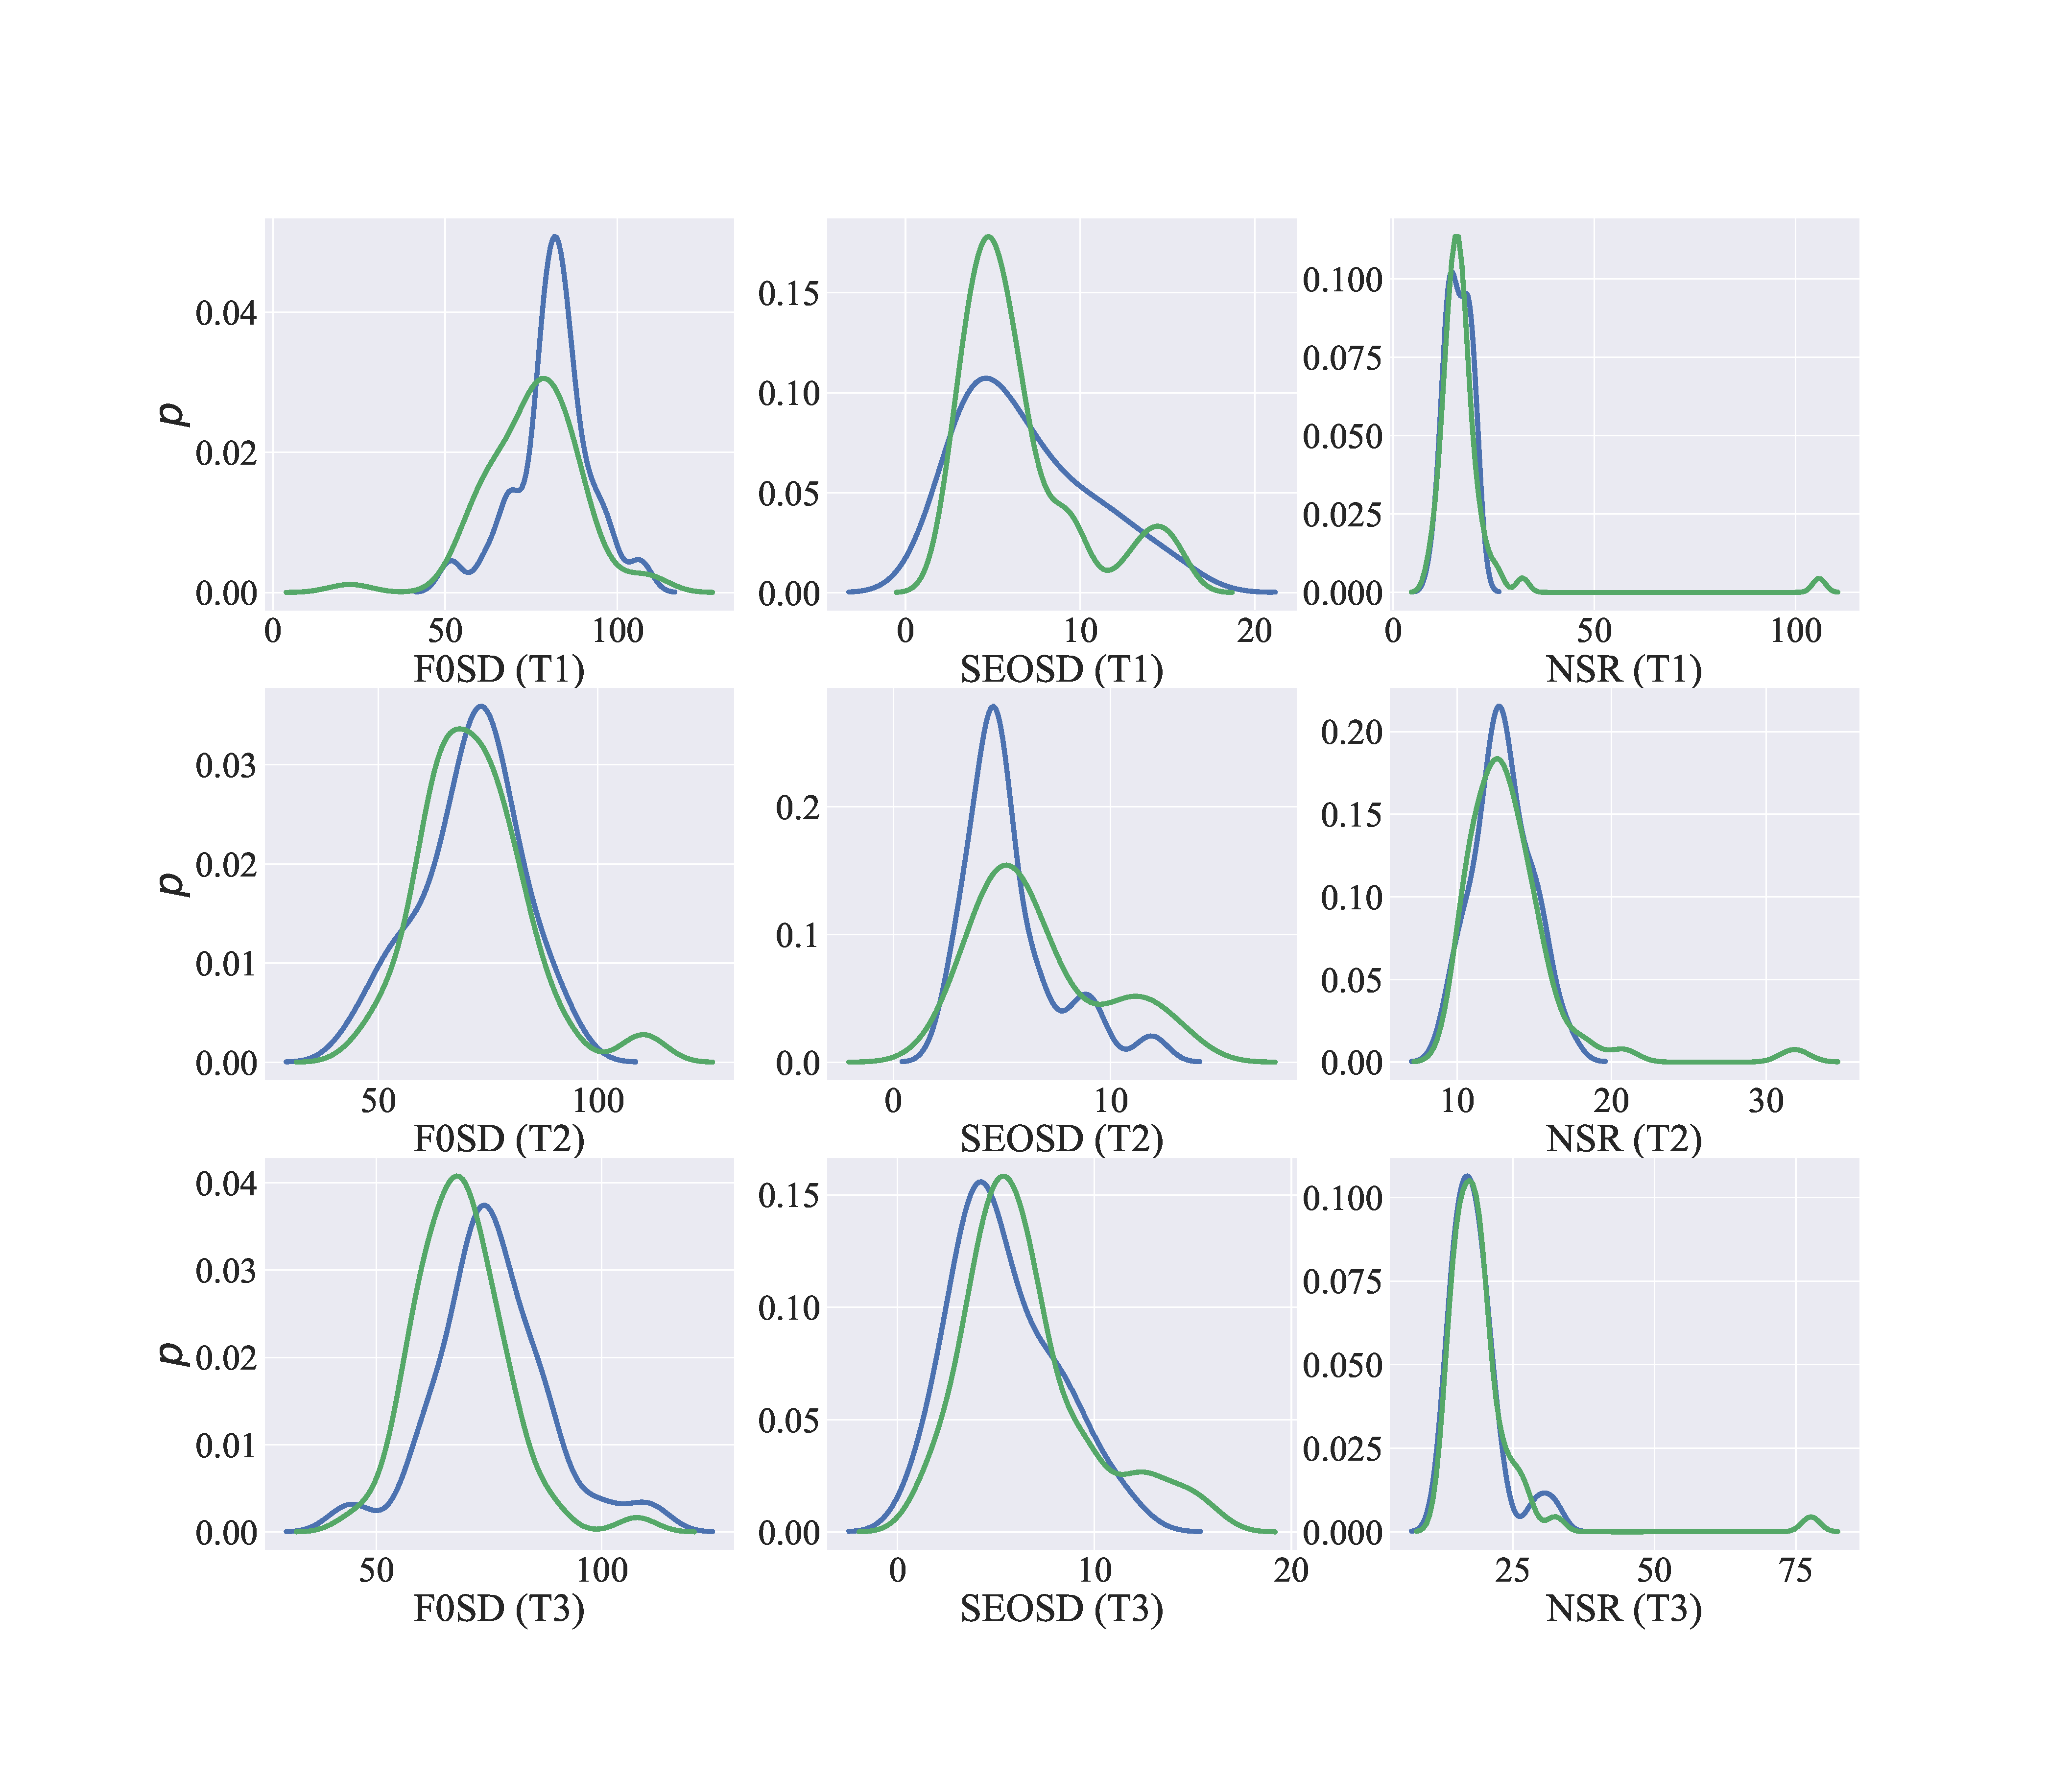
\includegraphics[width=0.99\textwidth]{pictures/ch4_comparisons_males.eps}
	\caption[Density estimation plots for male speakers.]{Density estimation plots (computed using kernel probability density estimation with Gaussian kernels) for selected acoustic features for all three speech tasks performed by male speakers only: T1\,--\,poem recitation task (first row); T2\,--\,emotionally-neutral reading (second row); and T3\,--\,stress-modified reading (third row). Colour notation: blue colour represents healthy speakers, and green colour represents speakers with PD. Feature notation: F0SD (standard deviation of fundamental frequency) expresses variability of intonation (melody of speech); SEOSD (standard deviation of squared energy operator) expresses variability of speech intensity (melody of speech); and NSR (net speech rate) expresses the number of phones per entire duration of speech without pauses (speech rate).}
	\label{fig:ch4_comparisons_males}
\end{figure}

\begin{figure}[htb!]
	\centering
	\scriptsize
	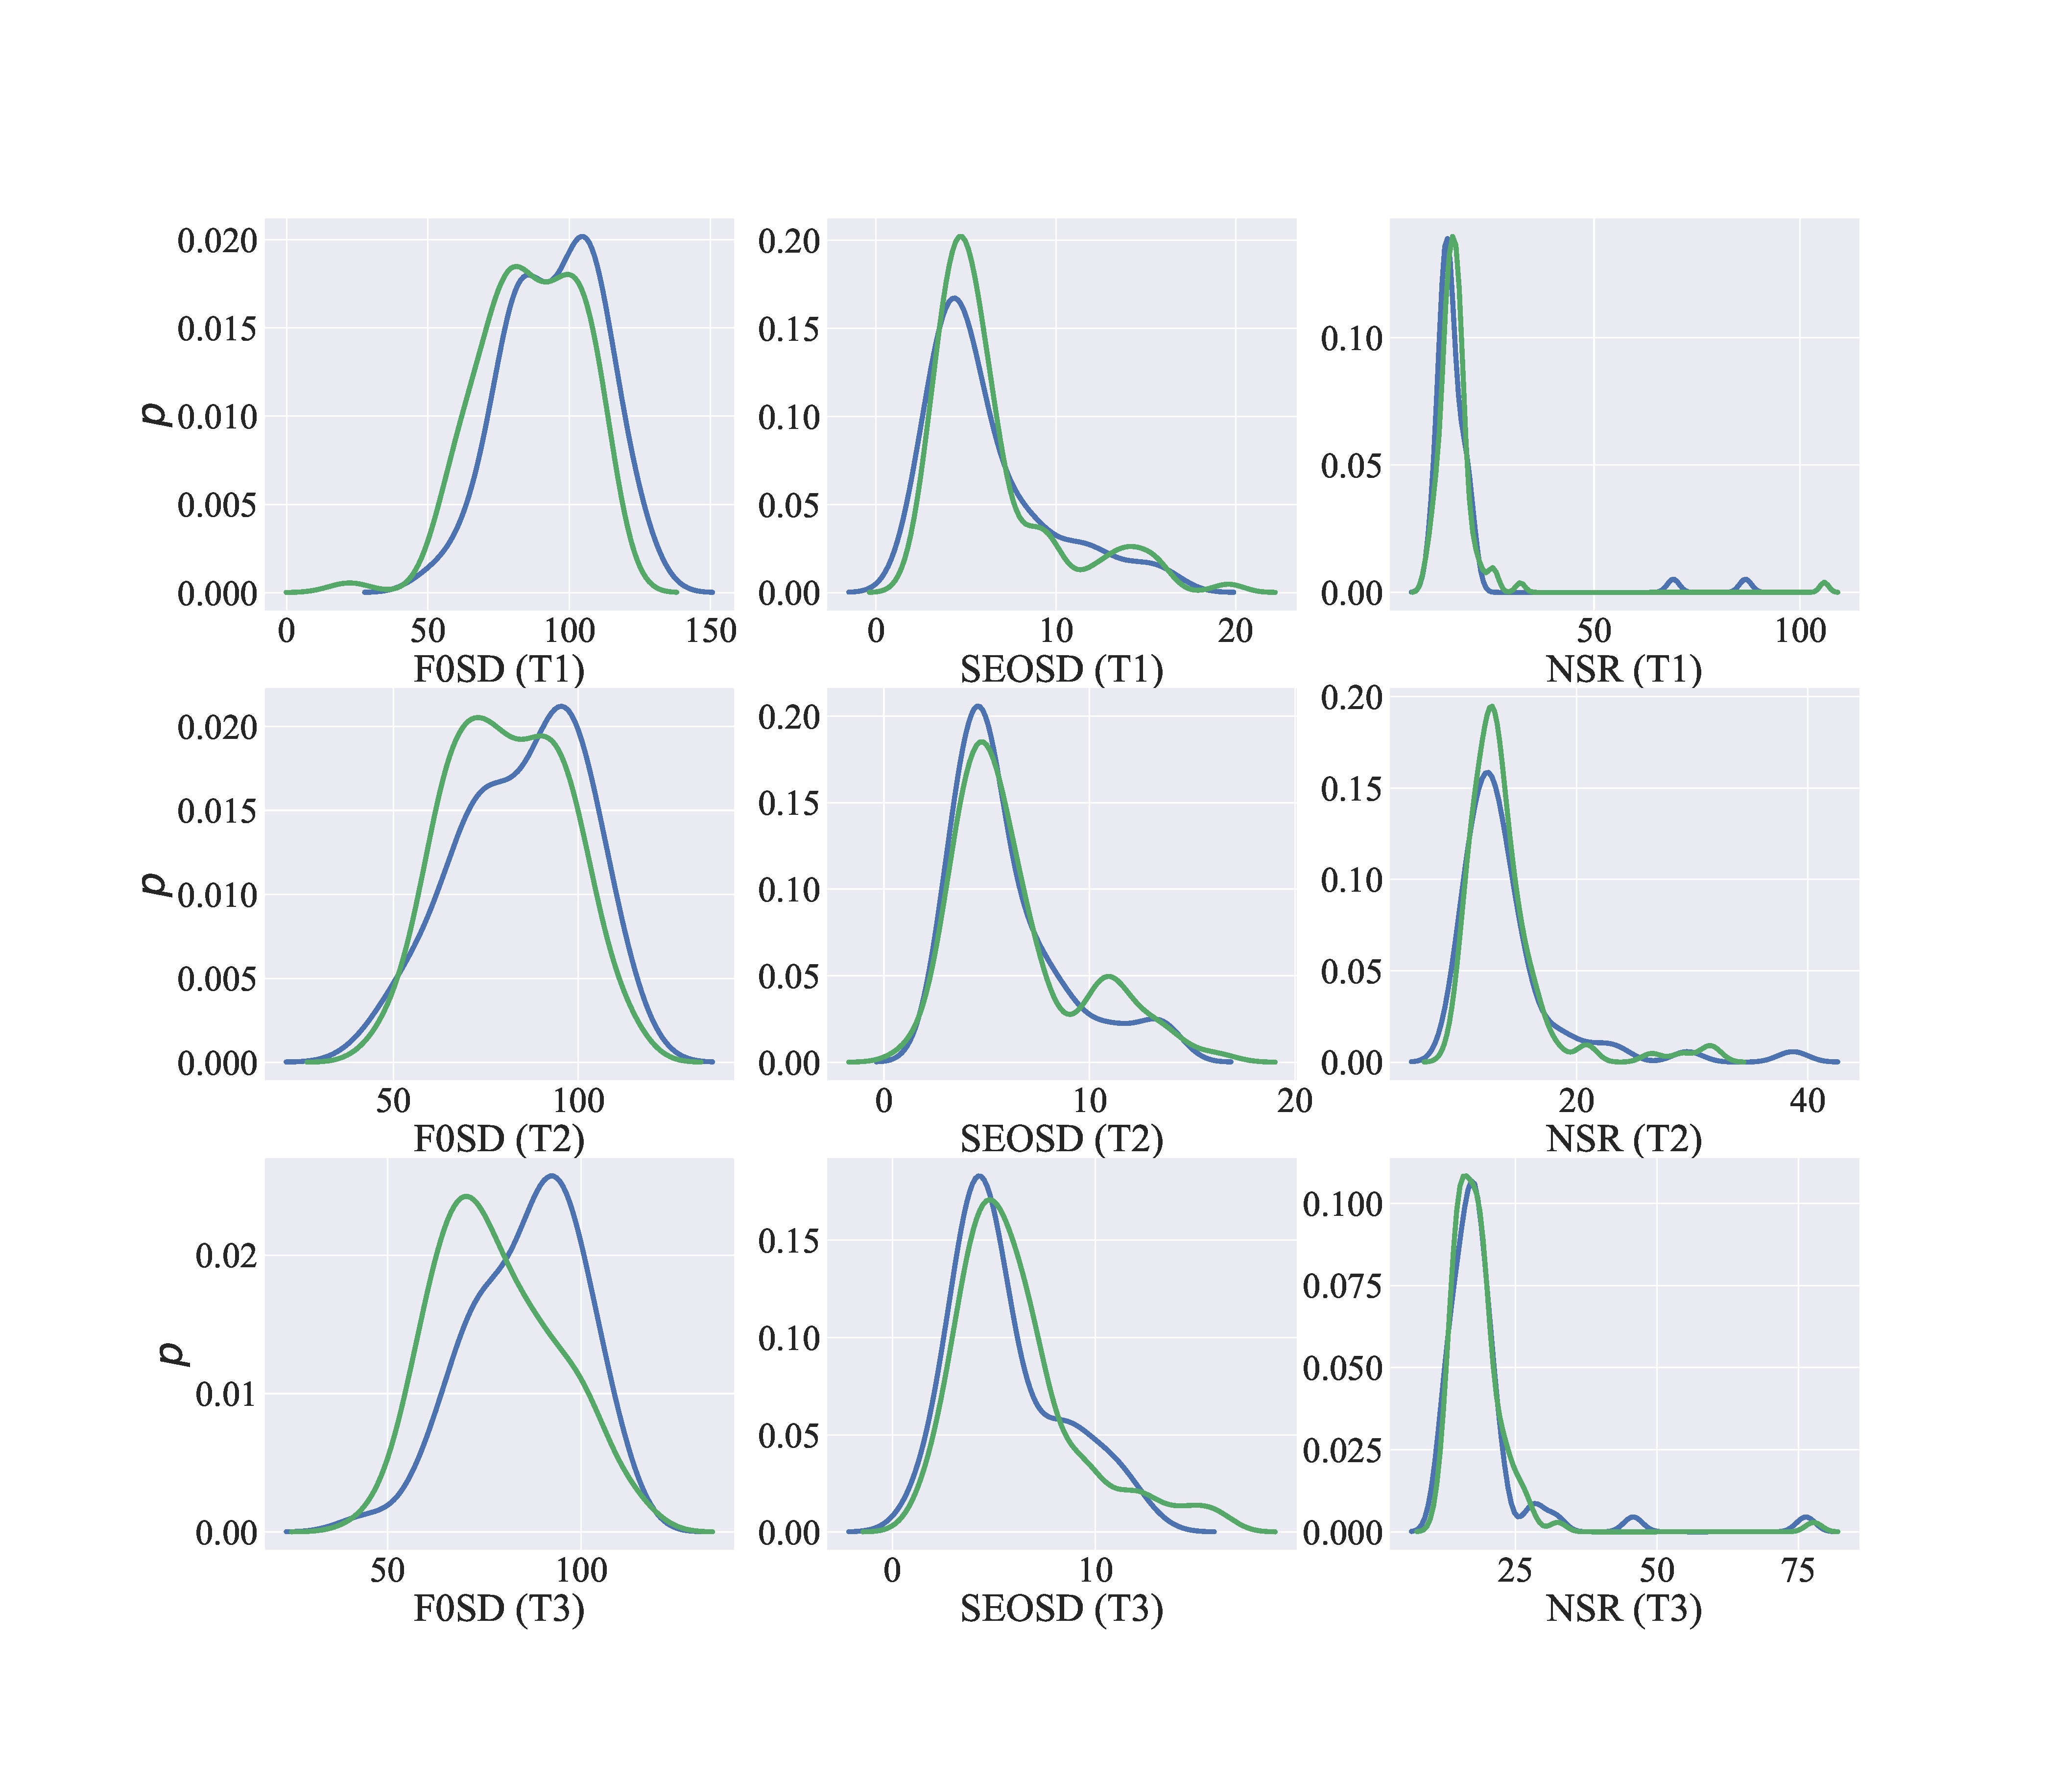
\includegraphics[width=0.99\textwidth]{pictures/ch4_comparisons_all.eps}
	\caption[Density estimation plots for all speakers.]{Density estimation plots (computed using kernel probability density estimation with Gaussian kernels) for selected acoustic features for all three speech tasks performed by all speakers (both genders combined): T1\,--\,poem recitation task (first row); T2\,--\,emotionally-neutral reading (second row); and T3\,--\,stress-modified reading (third row). Colour notation: blue colour represents healthy speakers, and green colour represents speakers with PD. Feature notation: F0SD (standard deviation of fundamental frequency) expresses variability of intonation (melody of speech); SEOSD (standard deviation of squared energy operator) expresses variability of speech intensity (melody of speech); and NSR (net speech rate) expresses the number of phones per entire duration of speech without pauses (speech rate).}
	\label{fig:ch4_comparisons_all}
\end{figure}

As can be seen in Table~\ref{tab:ch4_statistical_analysis}, when the extracted prosodic features are taken individually, the resulting classification performance of the trained models does not reach satisfactory level of accuracy. However, this is somewhat expected since dysprosody in HD is rarely expressed as manifestation in a~single prosodic domain. It is rather a~combination of monopitch, monoloudness and abnormalities in speech rate and pausing. And moreover, HD is also known to be manifested slightly differently from patient to patient, which makes the prediction task even more difficult. Nevertheless, the univariate models can at least provide an indication about the contribution of each of the selected acoustic features to discrimination of dysarthric and healthy speech. So, taking the previously mentioned facts into account, a~feature selection procedure was applied as the next step towards obtaining a~parsimonious, information-rich subsets of features, which provide maximum clinical information about the underlying prosodic pathology in patients with PD. Subsequently, the multivariate models were built using the selected features. The classification performance of these models can be seen in Table~\ref{tab:ch4_classification_groups}, and Table~\ref{tab:ch4_classification_combination}, respectively.

Consequently, t-distributed stochastic neighbourhood embedding (t-SNE)~\cite{Maaten2008} algorithm was used to visualize the multi-dimensional space of prosodic features in the two-dimensional one. For this purpose, all the extracted acoustic features were used. The visualization was performed for all the three speech tasks separately to show the clusters of healthy and dysarthric speakers when speech prosody is quantified in a~robust way (i.\,e. monopitch, monoloudness, and speech rate/pausing abnormalities are described altogether). This method was also applied for female speakers, male speakers, and all speakers (both genders combined). The results of this method are presented in Figure~\ref{fig:ch4_tsne}. As can be seen, using the prosodic description it is not strong enough to conclusively and definitely identify HD in patients with PD. It is important to stress the fact that the results are strongly related to the dataset used in this study. This claim is therefore based on the limited number of samples and must be considered as an approximation of the reality.

\begin{table*}[htb!]
	\centering
	\begin{threeparttable}
		\caption{Classification results for groups of acoustic features.}
		\label{tab:ch4_classification_groups}
		\footnotesize
		\centering
		\begin{tabular}{c l c c c c c c} 
			
			\hline\hline\noalign{\smallskip}
			\rowcolor{gray_table}
			feat. & gender & MCC & ACC & SEN & SPE & $p$ & No. \\
			\noalign{\smallskip}
			\multicolumn{8}{c}{Poem recitation} \\
			\noalign{\smallskip}\hline\noalign{\smallskip}
			
			% Monopitch model
			\multirow{3}{*}{F1} &
			  females & 0.14~$\pm$~0.38 & 58.04~$\pm$~17.71 & 63.00~$\pm$~25.87 & 50.33~$\pm$~32.73 & 0.0910 & 3 \\
			& males   & 0.19~$\pm$~0.39 & 58.15~$\pm$~19.01 & 57.06~$\pm$~24.90 & 61.00~$\pm$~33.94 & 0.0840 & 1 \\
			& all     & 0.17~$\pm$~0.26 & 59.33~$\pm$~12.43 & 61.35~$\pm$~14.68 & 55.53~$\pm$~21.15 & 0.1690 & 1 \\
			\noalign{\smallskip}
			
			% Monoloudness model
			\multirow{3}{*}{F2} &
			  females & 0.24~$\pm$~0.40 & 61.28~$\pm$~18.47 & 59.50~$\pm$~27.14 & 63.66~$\pm$~28.70 & 0.2590 & 8 \\
			& males   & 0.26~$\pm$~0.41 & 65.93~$\pm$~17.78 & 72.06~$\pm$~20.38 & 53.33~$\pm$~34.17 & 0.0090 & 6 \\
			& all     & 0.23~$\pm$~0.27 & 62.78~$\pm$~12.58 & 66.24~$\pm$~16.70 & 56.40~$\pm$~25.64 & 0.0020 & 3 \\
			\noalign{\smallskip}
			
			% Speech rate model
			\multirow{3}{*}{F3} &
			  females & 0.19~$\pm$~0.43 & 59.28~$\pm$~20.25 & 60.00~$\pm$~27.66 & 58.66~$\pm$~30.53 & 0.0790 & 2 \\
			& males   & 0.29~$\pm$~0.42 & 63.49~$\pm$~20.05 & 61.73~$\pm$~24.04 & 67.66~$\pm$~32.54 & 0.0130 & 1 \\
			& all     & 0.27~$\pm$~0.24 & 64.02~$\pm$~11.35 & 65.80~$\pm$~19.08 & 61.00~$\pm$~24.55 & 0.0010 & 1 \\
			\noalign{\smallskip}
			
			\noalign{\smallskip}\hline\noalign{\smallskip}
			\multicolumn{8}{c}{Reading with neutral emotion} \\
			\noalign{\smallskip}\hline\noalign{\smallskip}
			
			% Monopitch model
			\multirow{3}{*}{F1} &
			  females & 0.13~$\pm$~0.42 & 54.85~$\pm$~19.35 & 49.50~$\pm$~28.34 & 63.33~$\pm$~31.22 & 0.1450 & 3 \\
			& males   & 0.11~$\pm$~0.33 & 59.39~$\pm$~13.56 & 65.60~$\pm$~17.45 & 45.33~$\pm$~32.12 & 0.1340 & 2 \\
			& all     & 0.08~$\pm$~0.24 & 54.67~$\pm$~11.19 & 56.68~$\pm$~17.85 & 50.86~$\pm$~24.79 & 0.5910 & 3 \\
			\noalign{\smallskip}
			
			% Monoloudness model
			\multirow{3}{*}{F2} &
			  females & 0.16~$\pm$~0.44 & 58.19~$\pm$~20.29 & 59.50~$\pm$~28.07 & 56.00~$\pm$~31.90 & 0.1590 & 3 \\
			& males   & 0.37~$\pm$~0.42 & 70.53~$\pm$~19.62 & 74.60~$\pm$~20.34 & 62.33~$\pm$~30.64 & 0.0080 & 4 \\
			& all     & 0.19~$\pm$~0.28 & 60.90~$\pm$~13.00 & 63.97~$\pm$~15.55 & 55.33~$\pm$~23.27 & 0.1420 & 3 \\
			\noalign{\smallskip}
			
			% Speech rate model
			\multirow{3}{*}{F3} &
			  females & 0.30~$\pm$~0.37 & 64.04~$\pm$~17.63 & 65.00~$\pm$~25.25 & 62.66~$\pm$~29.84 & 0.0510 & 2 \\
			& males   & 0.20~$\pm$~0.31 & 60.31~$\pm$~15.40 & 61.73~$\pm$~20.89 & 58.00~$\pm$~26.98 & 0.0710 & 1 \\
			& all     & 0.12~$\pm$~0.30 & 56.17~$\pm$~13.89 & 56.53~$\pm$~15.02 & 55.80~$\pm$~23.82 & 0.3260 & 4 \\
			\noalign{\smallskip}
			
			\noalign{\smallskip}\hline\noalign{\smallskip}
			\multicolumn{8}{c}{Stress-modified reading} \\
			\noalign{\smallskip}\hline\noalign{\smallskip}
			
			% Monopitch model
			\multirow{3}{*}{F1} &
			  females & 0.31~$\pm$~0.35 & 64.38~$\pm$~15.63 & 67.50~$\pm$~25.87 & 60.33~$\pm$~30.84 & 0.0990 & 2 \\
			& males   & 0.21~$\pm$~0.38 & 61.74~$\pm$~17.71 & 63.80~$\pm$~21.02 & 57.66~$\pm$~31.26 & 0.1280 & 2 \\
			& all     & 0.15~$\pm$~0.26 & 58.37~$\pm$~13.13 & 61.60~$\pm$~17.21 & 52.73~$\pm$~19.60 & 0.1560 & 2 \\
			\noalign{\smallskip}
			
			% Monoloudness model
			\multirow{3}{*}{F2} &
			  females & 0.40~$\pm$~0.26 & 69.66~$\pm$~12.01 & 72.00~$\pm$~21.21 & 65.66~$\pm$~26.60 & 0.0240 & 3 \\
			& males   & 0.24~$\pm$~0.41 & 63.30~$\pm$~18.24 & 64.73~$\pm$~20.68 & 59.66~$\pm$~33.51 & 0.0360 & 4 \\
			& all     & 0.20~$\pm$~0.21 & 61.95~$\pm$~9.15  & 66.35~$\pm$~13.55 & 53.86~$\pm$~21.57 & 0.1150 & 2 \\
			\noalign{\smallskip}
			
			% Speech rate model
			\multirow{3}{*}{F3} &
			  females & 0.15~$\pm$~0.39 & 58.90~$\pm$~15.39 & 63.50~$\pm$~19.69 & 51.66~$\pm$~35.99 & 0.4570 & 2 \\
			& males   & 0.24~$\pm$~0.32 & 64.44~$\pm$~14.19 & 68.73~$\pm$~18.64 & 55.66~$\pm$~30.41 & 0.0650 & 1 \\
			& all     & 0.13~$\pm$~0.25 & 58.15~$\pm$~12.36 & 62.02~$\pm$~17.18 & 51.13~$\pm$~21.88 & 0.6840 & 2 \\
			\noalign{\smallskip}
			
			\noalign{\smallskip}\hline\hline
		\end{tabular}
		
		\begin{tablenotes}
			\scriptsize
			\item Table notation: F1\,--\,monopitch features; F2\,--\,monoloudness features; F3\,--\,speech rate features; F4\,--\,general prosodic features; MCC\,--\,Matthew's correlation coefficient (dimensionless)~\cite{Matthews1975}; ACC\,--\,classification accuracy (expressed in $\%$); SEN\,--\,classification sensitivity (expressed in $\%$); SPE\,--\,classification specificity (expressed in $\%$); No.\,--\,number of selected features; $p$\,--\,p-values of classification calculated by permutation test ($1000$ permutations).
		\end{tablenotes}
	\end{threeparttable}
\end{table*}

\begin{table*}[htb!]
	\centering
	\begin{threeparttable}
		\caption{Classification results for all acoustic features.}
		\label{tab:ch4_classification_combination}
		\footnotesize
		\centering
		\begin{tabular}{c l c c c c c c} 
		
			\hline\hline\noalign{\smallskip}
			\rowcolor{gray_table}
			feat. & gender & MCC & ACC & SEN & SPE & $p$ & No. \\
			\noalign{\smallskip}\hline\noalign{\smallskip}

			\multirow{3}{*}{T1} &
			  females & 0.36~$\pm$~0.42 & 66.57~$\pm$~19.80 & 66.00~$\pm$~25.13 & 68.33~$\pm$~30.90 & 0.0070 & 5 \\
			& males   & 0.35~$\pm$~0.34 & 67.84~$\pm$~17.33 & 68.93~$\pm$~22.54 & 66.00~$\pm$~27.34 & 0.0020 & 3 \\
			& all     & 0.33~$\pm$~0.16 & 67.30~$\pm$~08.42 & 68.84~$\pm$~14.18 & 64.66~$\pm$~14.98 & 0.0040 & 1 \\
			\noalign{\smallskip}

			\multirow{3}{*}{T2} &
			  females & 0.37~$\pm$~0.40 & 68.47~$\pm$~18.64 & 72.00~$\pm$~26.06 & 63.33~$\pm$~31.94 & 0.2110 & 3 \\
			& males   & 0.38~$\pm$~0.29 & 69.52~$\pm$~14.02 & 70.40~$\pm$~18.93 & 68.00~$\pm$~26.90 & 0.0050 & 8 \\
			& all     & 0.16~$\pm$~0.32 & 59.62~$\pm$~15.80 & 64.93~$\pm$~18.77 & 50.13~$\pm$~21.36 & 0.0350 & 4 \\
			\noalign{\smallskip}

			\multirow{3}{*}{T3} &
			  females & 0.42~$\pm$~0.35 & 70.71~$\pm$~16.24 & 71.00~$\pm$~19.13 & 70.33~$\pm$~30.91 & 0.0001 & 1 \\
			& males   & 0.37~$\pm$~0.34 & 70.03~$\pm$~16.05 & 73.53~$\pm$~19.28 & 63.00~$\pm$~29.41 & 0.0120 & 5 \\
			& all     & 0.25~$\pm$~0.26 & 63.20~$\pm$~12.44 & 65.06~$\pm$~14.92 & 60.00~$\pm$~21.07 & 0.0130 & 3 \\	

			\noalign{\smallskip}\hline\hline
		\end{tabular}
				
		\begin{tablenotes}
			\scriptsize
			\item Table notation: T1\,--\,poem recitation task; T2\,--\,reading with neutral emotion; T3\,--\,stress-modified reading task; MCC\,--\,Matthew's correlation coefficient (dimensionless)~\cite{Matthews1975}; ACC\,--\,classification accuracy (expressed in $\%$); SEN\,--\,classification sensitivity (expressed in $\%$); SPE\,--\,classification specificity (expressed in $\%$); No.\,--\,number of selected features; $p$\,--\,p-values of classification calculated by permutation test ($1000$ permutations).
		\end{tablenotes}
	\end{threeparttable}
\end{table*}

\begin{figure}[htb!]
	\centering
	\scriptsize
	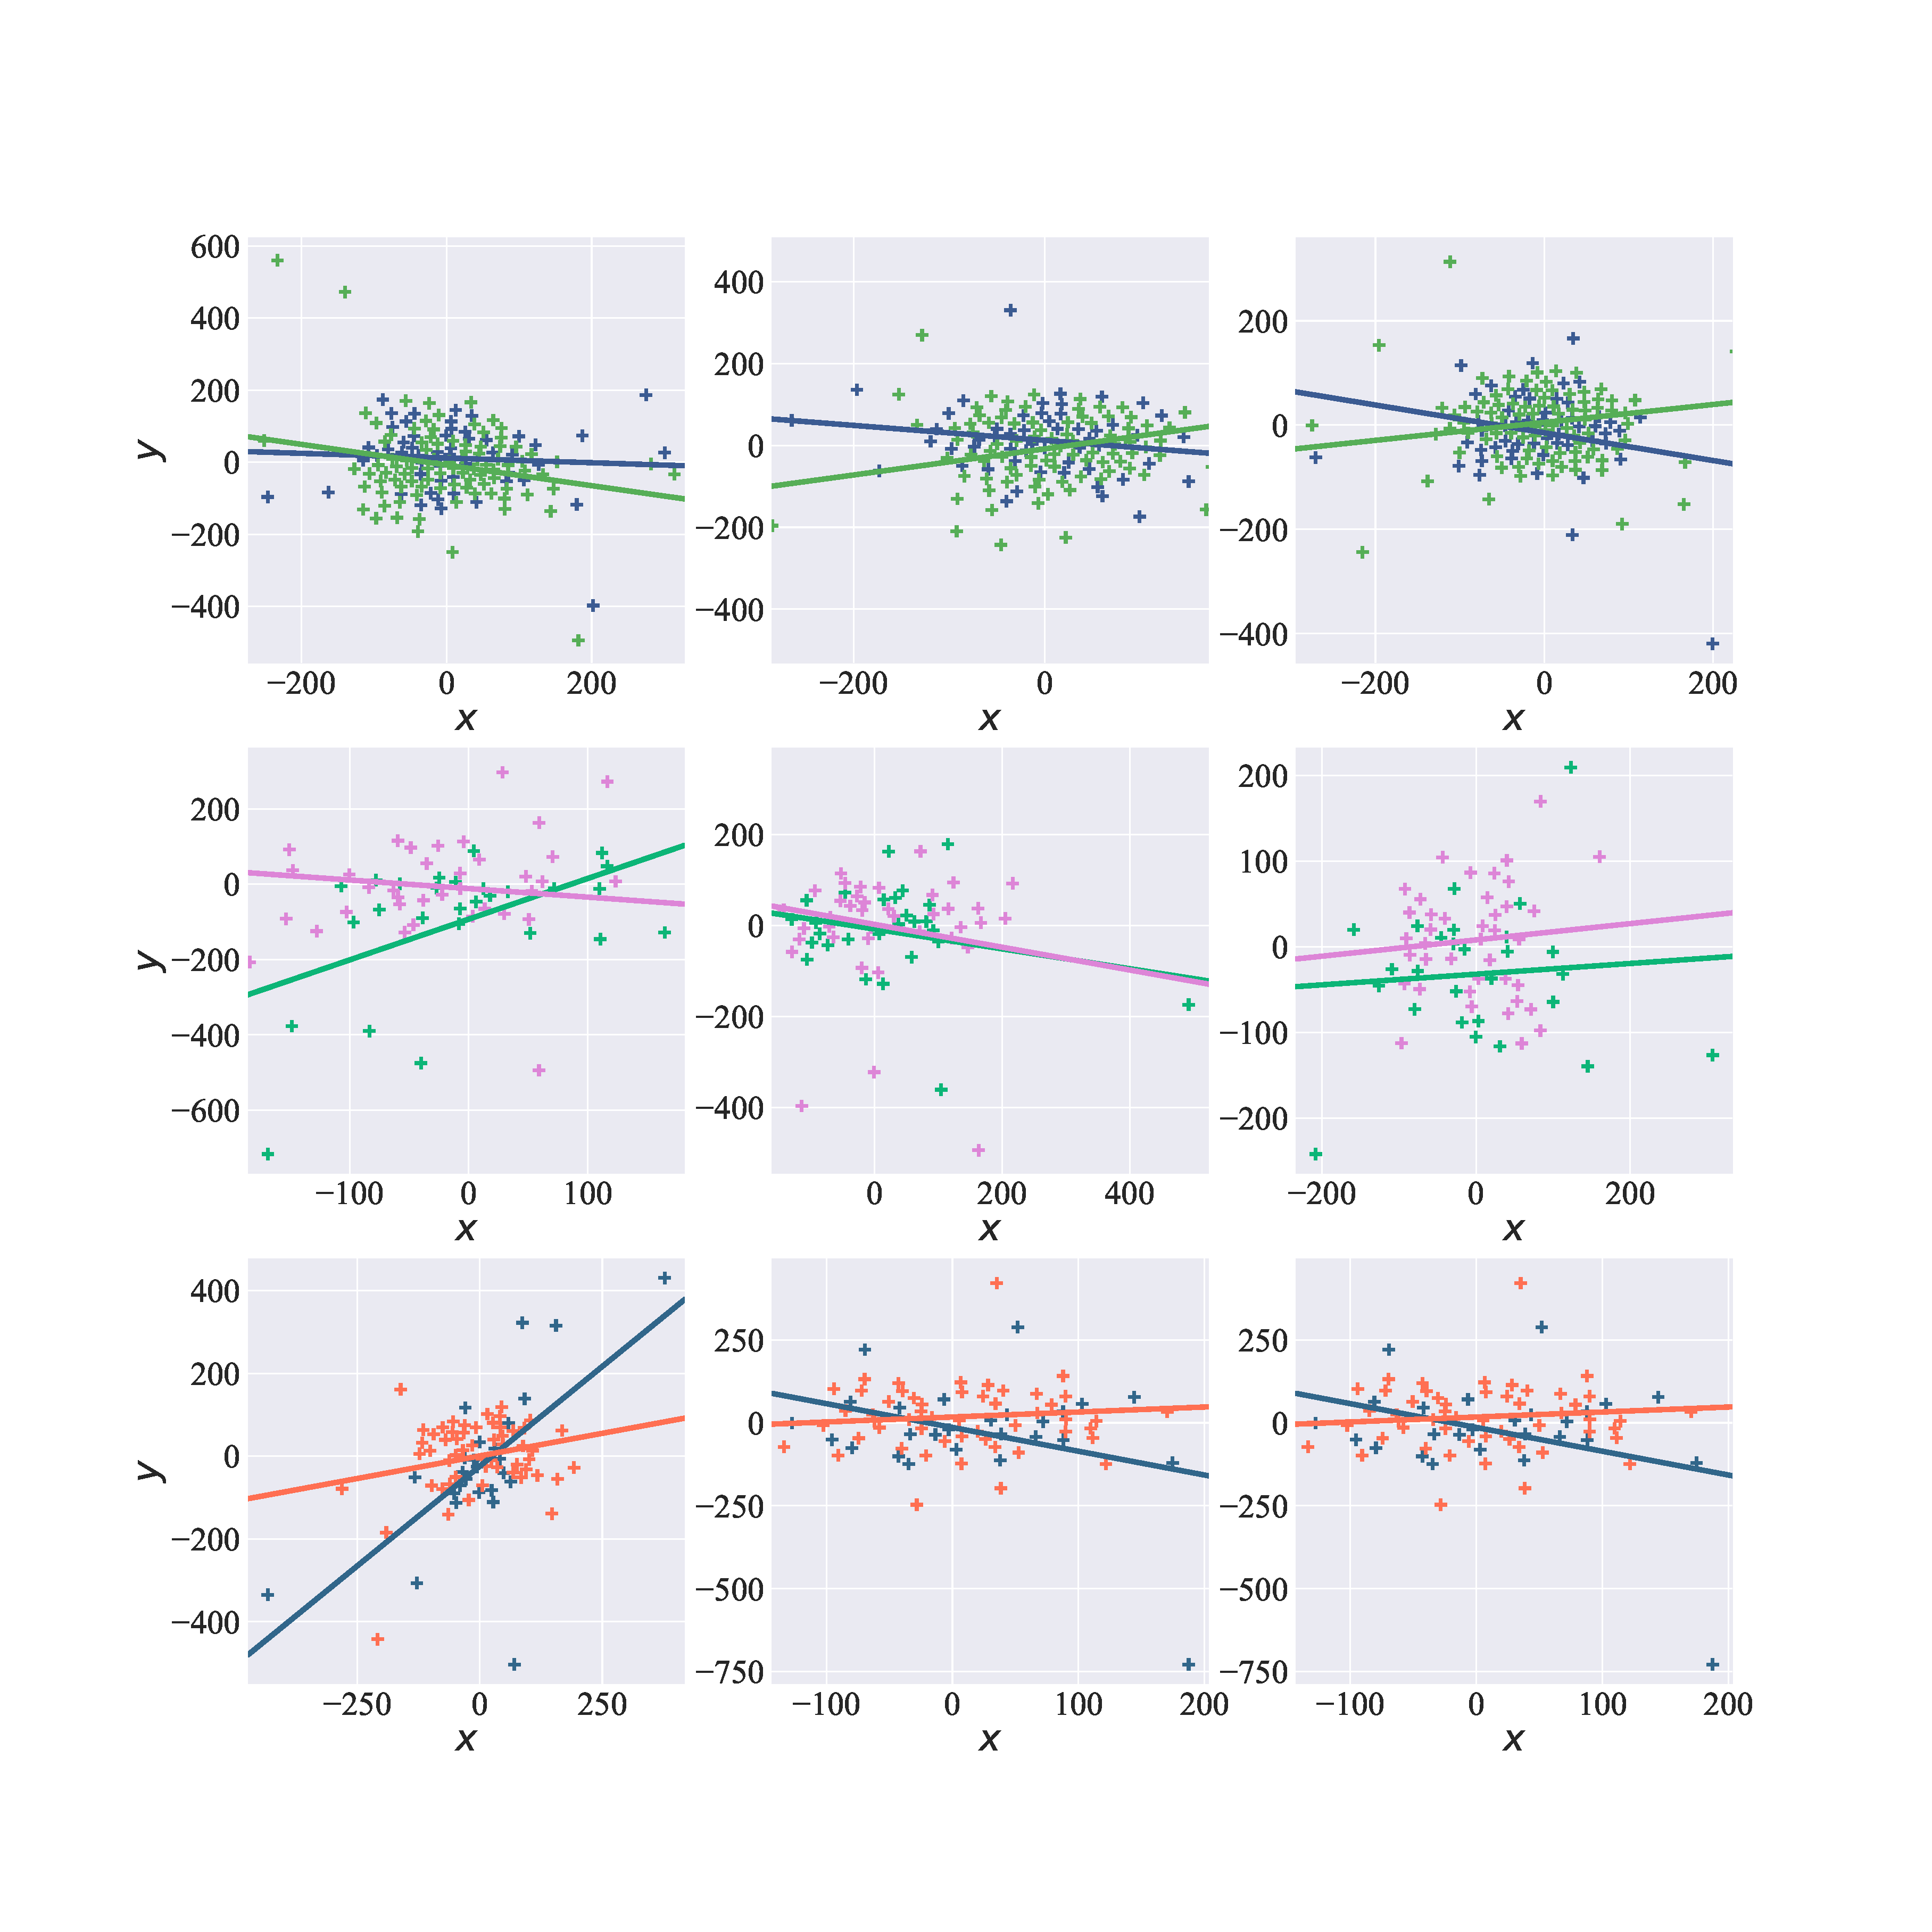
\includegraphics[width=0.99\textwidth]{pictures/ch4_tsne_separated.eps}
	\caption[t-distributed stochastic neighbourhood embedding visualization.]{Visualization of t-distributed stochastic neighbourhood embedding applied on all samples and acoustic features for each of the speech tasks separately (lines fitted using robust linear regression for each visualized class are provided as well). Graph grid notation: $1$. row\,--\,all speakers, $2$. row\,--\,female speakers, $3$. row\,--\,male speakers; $1$. column\,--\,poem recitation task, $2$. column\,--\,emotionally-neutral reading, $3$. column\,--\,stress-modified reading. Colour notation: all speakers\,--\,dark blue colour represents healthy speakers, and dark green colour represents speakers with PD; female speakers\,--\,medium green colour represents healthy speakers, and purple colour represents speakers with PD; and male speakers\,--\,medium blue colour represents healthy speakers, and orange colour represents speakers with PD. Note: the feature space is reduced from multi-dimensional space to two-dimensional one and therefore only general $x$, $y$ features are used to describe the resulting feature space.}
	\label{fig:ch4_tsne}
\end{figure}

\newpage
To specify the results presented in these two tables: Table~\ref{tab:ch4_classification_groups} shows the results of the multivariate classification analysis employed on the subsets of the prosodic features. Specifically, models for monopitch (F1), monoloudness (F2), and speech rate abnormalities (F3) were built. The assumption behind this approach was that despite insufficiency of the univariate models, investigation of the classification performance of each of the prosodic manifestations in HD can improve the performance of the models when more features are being used (it needs to be pointed out that these features do however describe the same phenomenon so that they are quiet correlated. But as mentioned previously, RF classifier is robust in dealing with high-dimensional and highly correlated data). Table~\ref{tab:ch4_classification_combination} shows the results of the multivariate classification analysis employed on all of the prosodic features (F4).

The best classification performance in terms of classification accuracy achieved using the prosodic features for each speech task separately can be summarized as follows: a) poem recitation task\,--\,$\mbox{ACC}=67.84\,\%$ the model was trained using only $3$ features based on the analysis of general prosodic impairment (TPT, TEOSD, SEOSD) computed for male participants; b) reading with neutral emotion\,--\,$\mbox{ACC}=69.52\,\%$, the model was trained using $8$ features based based on the analysis of general prosodic impairment (SEOSD, relF0SD, TST, TPT, relSEOSD, TPT\,(50\,ms), relSEOVR, NSR) computed for male participants; and finally c) stress-modified reading\,--\,$\mbox{ACC}=70.71\,\%$, the model was trained using just a~single feature based on the analysis of monoloudness (relTEOVR) computed for female participants. It is worth noting that some of these models did not achieve sufficiently low p-values of the permutation test (strict significance level of $0.01$ was chosen) that is needed to reject the null hypothesis. This may indicated that more data are required in order to get significant results~\cite{Golland2005}.

With respect to the models built for the subsets of the prosodic features and all of the features taken together (general prosodic model), the following classification performance was achieved: F1\,--\,$\mbox{ACC}=64.38\,\%$, the model was trained using prosodic features extracted from the stress-modified reading task performed by female participants; F2\,--\,$\mbox{ACC}=70.54\,\%$, the model was trained using prosodic features extracted from the reading task with neutral emotion performed by male participants; F3\,--\,$\mbox{ACC}=64.44\,\%$, the model was trained using prosodic features extracted from the stress-modified reading task performed by male participants; and finally F4\,--\,$\mbox{ACC}=70.71\,\%$, the model was trained using prosodic features extracted from the stress-modified reading task performed by male participants.

\section{Conclusion}
\label{ch4_5}

According to the literature \cite{Ho1998, Goberman2005d}, speech task used for the assessment of voice and speech has a~great impact on the prosodic aspects of HD. Moreover, as stated by Skodda et al. in $2011$, some aspects of prosody might be different in natural conversational speech in comparison to other speech tasks. Thus, in the frame of this study, three types of speech tasks are used: a) reading with neutral emotion\,--\,to obtain data comparable with previous studies \cite{Skodda2008, Skodda2010, Skodda2011c, Rusz2011} that also used speech tasks focusing on reading with neutral emotion in their analysis setup. To some extent the results are also comparable with the work of Bandini et al.~\cite{Bandini2015} that focused on the automatic identification of dysprosody in HD using a~sentence repetition task; b) stress-modified reading\,--\,to obtain data that are at least partially comparable with those proposed in the research of Tykalova et al.~\cite{Tykalova2014} focused on the acoustic investigation of stress patterns in PD using a~reading task. But the main idea behind this approach was to expose speakers to additional prosodic demands, which in theory could emphasize the prosodic impairment in the group of PD patients as opposed to the HC.

Regarding the individual analysis of the selected acoustic features quantifying dysprosody in HD, the following conclusion can be made. At first, this study confirms previous finding of several renowned researchers \cite{Canter1965, Metter1986, Flint1992, Goberman2005b, Skodda2011c} reporting that patients with PD exhibit decreased intonation variability in comparison with HC (difference of approximately $8.72\,\%$). This pattern can be seen in almost every scenario used in this study except a~single reading task performed by the male participants with neutral emotion. This suggests that emotionally-neutral reading, especially in the male subjects is not sufficient enough to capture monopitch. In contrast, speech tasks such as stress-modified reading and a~recitation task seems to be a~good candidates for further investigation. Interestingly, at the same time, the results suggests that PD patients produce higher variability in speech intensity than HC (difference of approximately $12.41\,\%$), which is in contradiction with the previous findings published in \cite{Metter1986, Watson2008, Rusz2011, Skodda2011c}. However, this might be a~consequence of a~presence of so far uncovered gender-related pattern of speech intensity control impairment in HD, especially in the dataset used in the frame of this study, which is based on the observation of great gender-related distinctions of speech intensity deterioration summarized in Table~\ref{tab:ch4_comparisons}. Therefore, subsequent investigation of this phenomenon would be of interest. And finally, concerning speech rate abnormalities, the results suggest that PD patients in general produce lower speech rate that HC when performing a~task that requires prosodic demands such as stress or melody alternation. Regarding the gender-related distinctions, male participants seem to have have higher speech rate when compared to HC. Nevertheless, this is likely a~dataset-specific pattern that would need to be confirmed using a~different and possibly multilingual dataset.

Next, with respect to the comparison between emotionally-neutral and stress-modified reading. The following conclusion can be drawn: the classification accuracy achieved for the model based on the stress-modified reading performed by female speakers ($70.71\,\%$) and the model based on the emotionally-neutral reading performed by male speakers ($69.52\,\%$), may indicate no difference between these two tasks. However, deeper investigation considerably favours the stress-modified reading tasks considerably. The main reasons supporting this conclusion are: a) the p-value computed using permutation test is significantly lower in the case of stress-modified reading ($p=0.0001$) in contrast with the emotionally-neutral one ($p=0.0050$) suggesting higher reliability and statistical significance of the results; b) when the feature selection was applied, only a~single prosodic feature (relTEOVR) expressing monoloudness was needed to provide sufficient power to discriminate dysarthric and healthy speech, whereas eight features were selected in the case of emotionally-neutral reading task. Therefore, the clinical interpretability of the results derived from the reading with stress emphasis is far more convenient and practical. One more important aspect to consider is the fact that the two results also differ in their corresponding gender group. Nevertheless, in the case of emotionally-neutral reading, the results achieved for the group of female speakers are comparable to the ones achieved for the male group. Moreover, the statistical significance of this case was rejected anyway.

With respect to the comparison between the poem recitation task and the reading tasks, the results shows that the poem recitation task outperformed both reading tasks in the case of gender-undifferentiated analysis. This suggests that recitation-related rhythmical demands can in general lead to more precise discrimination of dysprosody in HD in cases when gender-differentiation is not required. In contrast to the straightforwardness of this outcome, the gender information consideration inflicted higher classification accuracy of stress-modifier reading compared to the poem recitation. One can hypothesize this may be a~consequence of some yet to be found gender-related pattern of rhythm and stress control deterioration present in HD. Furthermore, it is also important to emphasize the difference in gender group sizes (the mixed group contains approximately twice as many speakers than the gender-separated groups), therefore the difference in performance could be caused by an independent phenomena. Nevertheless, this hypothesis needs to be confirmed by the subsequent investigation. Another interesting observation made here is the striking proximity of the classification accuracies achieved by the emotionally-neutral reading and the poem recitation. Considering that when no prosodic demands such as rhythm, stress or emotion are required, marked superiority of the poem recitation would be naturally anticipated. Nevertheless, permutation test repeatedly gave disadvantage to the results achieved for the reading with neutral emotion.

Finally, When discriminating dysarthric and healthy speech using several scenarios focused on the expression of monopitch, monoloudness, speech rate abnormalities and a~combination of these prosodic flaws, the results showed that the analysis of a~single aspect of parkinsonian dysprosody (using this particular set of features) does not achieve sufficient classification accuracy, which is in some respect consistent with the results proposed by Lowit~\cite{Lowit2008} in $2008$ in which the author stated that a~combination of these aspects should be analysed exclusively. As can be seen in Table~\ref{tab:ch4_comparisons} this fact is also supported by the p-values computed using the permutation test that in most cases rejected the hypothesis of statistical significance of these prosodic sub-models. In contrast, the analysis of general prosodic features improved the classification accuracies of the models. Therefore, it can be concluded that future development of novel prosodic features quantifying the relationship between monopitch, monoloudness and speech rate disruption in PD is likely to bring deeper understanding of HD and its manifestation on human speech prosody.

To guarantee a~complete and relevant overview, limitations of this work need to be pointed out. With respect to the speech sample, one drawback (which is a~common one of many studies dealing with the acoustic analysis of speech in PD) is relatively small dataset restricting overall statistical significance of the results. Additionally, since the prevalence rate of PD is estimated to approximately $1.5\,\%$ (for people aged over 65 years, see~\cite{Rijk1997}), investigated data should reflect this fact. However, most dataset comprise more PD patients than healthy speakers, which therefore does not correspond with the reality. This is also the case of this particular work. Moreover, it is also worth noting that the current results are based upon speech tasks of relatively limited length. As suggested by Rusz et al. in~\cite{Rusz2013, Rusz2013b} acoustic features computed from a~running speech are the most prospective ones to assess the speech impairment in PD. So, an addition of the running speech can in general bring new insights into understanding of differences among neutral, stressed, rhymed and spontaneous speech in patients with PD. Finally, no correction of the p-values obtained by the Mann-Whitney U~test and Spearman's correlation was performed. However, since the tests were executed only on carefully selected set of $19$ prosodic features, the errors caused by the multiple testing issue are not as relevant as they could be if hundreds or thousands of features were used.

To summarize, the results confirms the previous findings of reduced pitch variation~\cite{Canter1963, Metter1986, Flint1992, Goberman2005b, Goberman2005d, Rusz2011}, to some extent impaired speech intensity control~\cite{Metter1986, Watson2008, Skodda2011c, Rusz2011, Clark2014} and speech rate abnormalities~\cite{Weismer1984, Metter1986, Skodda2008, Skodda2011c} in PD. The results also highlight the fact that more studies are necessary in order to fully understand the manifestation of HD on human prosody. In $2009$, Skodda et al.~\cite{Skodda2009} used prosodic features to study changes of speech rate and pitch variation in patients with PD over time and showed the presence of some characteristic changes in parkinsonian dysprosody. However, further longitudinal studies are required. Besides the PD classification and disease tracking, the analysis of dysprosody in HD can also be used during an evaluation of the modern non-invasive treatment methods such as high-frequency repetitive transcranial magnetic stimulation (rTMS)~\cite{Eliasova2013}, which has a~great potential in treatment of PD. 

\chapter[Assessment of Parkinson's disease]{Assessment of Parkinson's disease}
\label{ch5}

\section{State of knowledge}
\label{ch5_1}

Over the last few decades, objective paraclinical methods such as the analysis of digitized hand-writing~\cite{Drotar2014, Faundez-Zanuy2014, Drotar2015, Mucha2018a}, computerized freezing of gait evaluation~\cite{Factor2014, Rocha2014}, or the acoustic analysis of dysarthric speech~\cite{Mekyska2011b_eng, Eliasova2013, Mekyska2015, Smekal2015c} have been developed. In terms of PD, the studies in which such methods have been applied have focused mainly on parkinsonian symptoms identification, description of the relationships between motor and non-motor symptoms of the disease, overall severity of PD estimation, etc. In theory, voice/speech, movement (e.\,g. gait), hand-writing and similar actions/signals can be digitized and processed remotely on computer. After that, modern signal processing techniques, statistical analyses, and/or machine learning algorithms can be used to extract a~wide range of parameters that can be integrated into a~decision support system that can eventually be used in clinical practice to enable clinicians to use such data to support their decision making when diagnosing, assessing, or monitoring the progress of PD. However, to reach this point, more studies need to be performed. 

In terms of HD in PD (i.\,e. the hypothesis is that quantification of voice/speech deficits in HD can be used to indirectly assess other non-speech symptoms of PD), especially studies that bring more insight into pathological mechanisms behind a~variety of voice/speech disorders accompanying HD and other motor and non-motor symptoms of PD are yet to be employed. If such pathological mechanisms are present and precisely described, it is likely that carefully-planned and sensitive acoustic analysis of voice/speech can be used to assess these motor and non-motor symptoms, or possibly predict their future evolution in time. 

So, with these ideas in mind, clinical rating scales that are nowadays being commonly used to quantify motor and non-motor symptoms of PD such as Unified Parkinson's Disease Rating Scale (UPDRS)~\cite{Fahn1987}, Non-Motor Symptoms Scale (NMSS)~\cite{Chaudhuri2007}, Beck Depression Inventory (BDI)~\cite{Beck2000}, Freezing Of Gait questionnaire (FOG-Q)~\cite{Giladi2000}, The REM sleep Behaviour Disorder Screening Questionnaire (RBDSQ)~\cite{Stiasny2007}, Mini-Mental State Examination (MMSE)~\cite{Folstein1975} or Addenbrooke's Cognitive Examination-Revised (ACE-R)~\cite{Larner2007}, etc., can serve as relevant clinically-established baseline data, which can be used to model the relationship between speech disorders in HD and other non-speech symptoms of PD. The values of these scales can be mathematically modelled and the trained models can consequently be used to estimate the clinical status of the patients in a~non-invasive, paraclinical way that has a~great potential to be used for other related tasks such as prediction and monitoring of the efficiency of the treatments, etc.

With respect to the estimation of the scores quantifying parkinsonian manifestations, UPDRS, especially its third part (motor examination) \cite{Asgari2010, Bayestehtashk2015, Eskidere2012, Peterek2013, Tsanas2010, Tsanas2010a, Tsanas2010b}, or its total score \cite{Eskidere2012, Peterek2013, Tsanas2010, Tsanas2010a, Tsanas2010b} has been most commonly-used by researchers. In addition to UPDRS, Mekyska et al.~\cite{Smekal2015c} explored prediction capabilities of regression models estimating a~larger number of rating scales, specifically FOG-Q, NMSS, BDI, MMSE, and ACE-R. Finally, Rektorova et al. built regression models capable of predicting cognitive decline in PD patients based on the analysis of voice/speech signals~\cite{Rektorova2016}.

To summarize, there are some works investigating prediction of PD severity using acoustic analysis of dysarthric speech. However, the researchers have mostly been experimenting with acoustic features describing phonatory aspects of HD or aimed at robust parametrization~\cite{Mekyska2015, Smekal2015c} without specifically focusing on dysprosody (most prosody-specific analysis was proposed in~\cite{Rektorova2016}). In the previous study, it has been shown that dysprosody can be successfully used to identify HD in PD. Therefore, the hypothesis is that the same can be said in terms of PD assessment.

\section{Rationale behind the research}
\label{ch5_2}

To summarize and emphasize, relatively small number of studies evaluating possibilities of estimating severity of PD, assessed by a~variety of clinical scales rating motor and non-motor deficits present in PD, have been employed~\cite{Asgari2010, Bayestehtashk2015, Eskidere2012, Peterek2013, Tsanas2010, Tsanas2010a, Tsanas2010b, Smekal2015c, Rektorova2016, Galaz2018a}. Moreover, most of these works took only a~single rating scale (UPDRS), or a~phonatory aspects of HD into account. Even though, in $2015$, Mekyska et al. proposed a~study presenting estimation of much larger set of clinical rating scales using robust voice/speech parametrization~\cite{Mekyska2015}, more studies are needed to evaluate these results and/or come up with new insights. Finally, in $2016$, Rektorova et al.~\cite{Rektorova2016} showed for the first time that speech prosody might be used to estimate PD prognosis in~pilot prospective longitudinal study, in which the authors assessed how speech prosody impairment in PD in addition to other motor and non-motor features may predict global cognitive worsening or changes in the cognitive status from normal cognition to mild cognitive impairment (MCI) or from PD-MCI to PD dementia. Nevertheless, additional studies are needed to evaluate these results and to show whether speech prosody assessment might serve as a~good biomarker for predicting a~malignant course of the disease.

Therefore, the study presented in this thesis builds upon the previous finding and applies robust analysis of dysprosody in HD to indirectly estimate degree of PD severity assessed by a~large number of well-known and widely-used clinical rating scales. The reason behind this type of estimation is that perceptual assessment of PD severity even if performed by skilled clinicians is subject to inter-rater variability~\cite{Ramaker2002, Post2005}. In addition, auditory and visual perception of every rater is limited, and there is nothing to be done about that. Therefore, the hypothesis is that objective computerized quantification of voice/speech signals can provide clinicians with additional information supporting their evaluation. 

Moreover, as presented in Chapter~\ref{ch4}, the prosodic aspects in HD can be sufficiently described using speech tasks that require precise control of speech melody (recitation task) and/or stress (stress-modified reading). To build upon the results summarized in this study, this one uses the same set of speech tasks (poem recitation task, reading with neutral emotion, and stress-modified reading). As well as in the previously mentioned study concerning HD identification, the comparison of the prediction performance of regression models assessing PD severity is compared to evaluate the sufficiency of these speech task in this particular settings. Finally, Combination of the models is considered as well.

\section{Methodology}
\label{ch5_3}

\subsection{Description of the dataset}
\label{ch5_3_1}

In the frame of this study, robust analysis and estimation of motor and non-motor symptoms of idiopathic PD using the acoustic analysis of dysarthric speech were employed. These symptoms were evaluated by skilled neurologists and clinical psychologists who examined and rated each PD patient participating in this study according to a~variety of widely used and recognized clinical rating scales such as: UPDRS~III (evaluation of motor functions)~\cite{Fahn1987}; UPDRS~IV (evaluation of complications of therapy; Hoehn and Yahr scale, staging of severity of PD)~\cite{Fahn1987}; FOG-Q (evaluation of freezing and other gait-related deficits)~\cite{Giladi2000}; NMSS (evaluation of non-motor deficits)~\cite{Chaudhuri2007}; RBDSQ (evaluation of sleep disorders, especially in the REM sleep)~\cite{Stiasny2007}; ACE-R (evaluation of cognitive dysfunctions)~\cite{Larner2007}; MMSE (evaluation of cognitive dysfunctions)~\cite{Folstein1975}; and BDI (evaluation of depression) \cite{Beck2000, Beck1961}. These scales are nowadays being commonly used in the clinical practice to assess and rate the severity of motor and non-motor manifestations associated with PD. Other clinical rating scales exist as well. However, in the frame of this study, this exact subset of the rating scales is considered exclusively.

To follow the results summarized in the previous chapter, the same speech tasks, recording setup, dataset, etc. (database) were used. For more information see, Chapter~\ref{ch4} (Section~\ref{ch4_3_1}). However, in this particular study, only patients with PD are considered. Moreover, a~subset of the patients was needed to be selected. The reason for that is the necessity of having the complex clinical information about each of the patients. More specifically, not every patient did undergo all examinations so that for some patients full clinical status is not available. Hence, to ensure that no missing or corrupted data will be present in the dataset, a~subset of $72$ PD patients ($47$ males and a~group of $25$ females, characteristics described as mean (sd): participants' age in years $67.50$ ($8.08$); duration of the disease in years $7.47$ ($4.17$)) was selected. For more information about demographical and clinical characteristics of the used cohort, see Table~\ref{tab:ch5_clinical_data}.

\begin{table*}[htb!]
	\centering
	\begin{threeparttable}
		\caption{Clinical characteristics of the patients.}
		\label{tab:ch5_clinical_data}
		\footnotesize
		\centering
		\begin{tabular}{l r r r r r r r r r}

			\hline\hline\noalign{\smallskip}
			\rowcolor{gray_table}
			charact. & mean & std & min & Q1 & Q2 & Q3 & max & r\,(d) & r\,(s) \\
			\noalign{\smallskip}\hline\noalign{\smallskip}
			
			LED (mg/day) &  995.10 &  566.28 &    0.00 &  600.00 &  825.00 & 1325.50 & 2275.00 & 2275 &  $\infty$ \\
			UPDRS III    &   24.06 &   12.22 &    3.00 &   12.75 &   25.00 &   33.25 &   55.00 &   52 &  108 \\
			UPDRS IV     &    2.94 &    2.68 &    0.00 &    0.00 &    2.00 &    5.00 &    9.00 &    9 &   23 \\
			FOG-Q        &    6.46 &    5.63 &    0.00 &    1.00 &    5.50 &   10.00 &   20.00 &   20 &   24 \\
			NMSS         &   35.23 &   20.75 &    2.00 &   17.75 &   33.00 &   52.25 &   94.00 &   94 &  360 \\
			RBDSQ        &    3.67 &    3.13 &    0.00 &    1.00 &    3.00 &    5.00 &   13.00 &   13 &   13 \\
			ACE-R        &   87.33 &    8.02 &   60.00 &   82.75 &   87.00 &   93.00 &   99.00 &   39 &  100 \\
			MMSE         &   27.88 &    2.54 &   16.00 &   28.00 &   28.50 &   29.00 &   30.00 &   14 &   30 \\
			BDI          &   10.46 &    6.14 &    0.00 &    6.00 &    9.00 &   13.50 &   27.00 &   27 &   63 \\ 
			
			\noalign{\smallskip}\hline\hline
		\end{tabular}

		\begin{tablenotes}
			\scriptsize
			\item[1] Table notation: charact.\,--\,characteristics (clinical); Qx\,--\,x-th quartile (Q1\,[first], Q2\,[second], Q3\,[third]); r\,(d)\,--\,range (max\,$-$\,min) computed from the values actually present in the dataset; r\,(s)\,--\,range of the values in the scale; LED\,--\,L-dopa equivalent daily dose (mg/day)~\cite{Lee2010}; UPDRS~III\,--\,Unified Parkinson's disease rating scale, part~III: evaluation of motor function~\cite{Fahn1987}; UPDRS~IV\,--\,Unified Parkinson's disease rating scale, part~IV: evaluation of complications of therapy (Hoehn and Yahr scale, staging of severity of Parkinson's disease)~\cite{Fahn1987}; FOG-Q\,--\,Freezing of gait questionnaire~\cite{Giladi2000}; NMSS\,--\,Non-motor symptoms scale~\cite{Chaudhuri2007}; RBDSQ\,--\,The REM sleep behavior disorder screening questionnaire~\cite{Stiasny2007}; ACE-R\,--\,Addenbrooke's cognitive examination-revised~\cite{Larner2007}; MMSE\,--\,Mini-mental state examination~\cite{Folstein1975}; BDI\,--\,Beck depression inventory \cite{Beck2000, Beck1961}.
		\end{tablenotes}
	\end{threeparttable}
\end{table*}

Moreover, as in the previous study, descriptive statistical graphs of the selected clinical characteristics are used. The graphs show histograms (i.\,e. approximation of a~distribution of the values of the clinical rating scales in the sample), scatter plots (i.\,e. approximation of a~joint distribution of two clinical rating scales in the sample), estimation of the linear relationship (robust linear regression estimator) and the associated residuals between the clinical data assessed by the rating scales. The graphs can be seen in Figure~\ref{fig:ch5_clinical_statistics}.

\begin{figure}[htb!]
	\centering
	\scriptsize
	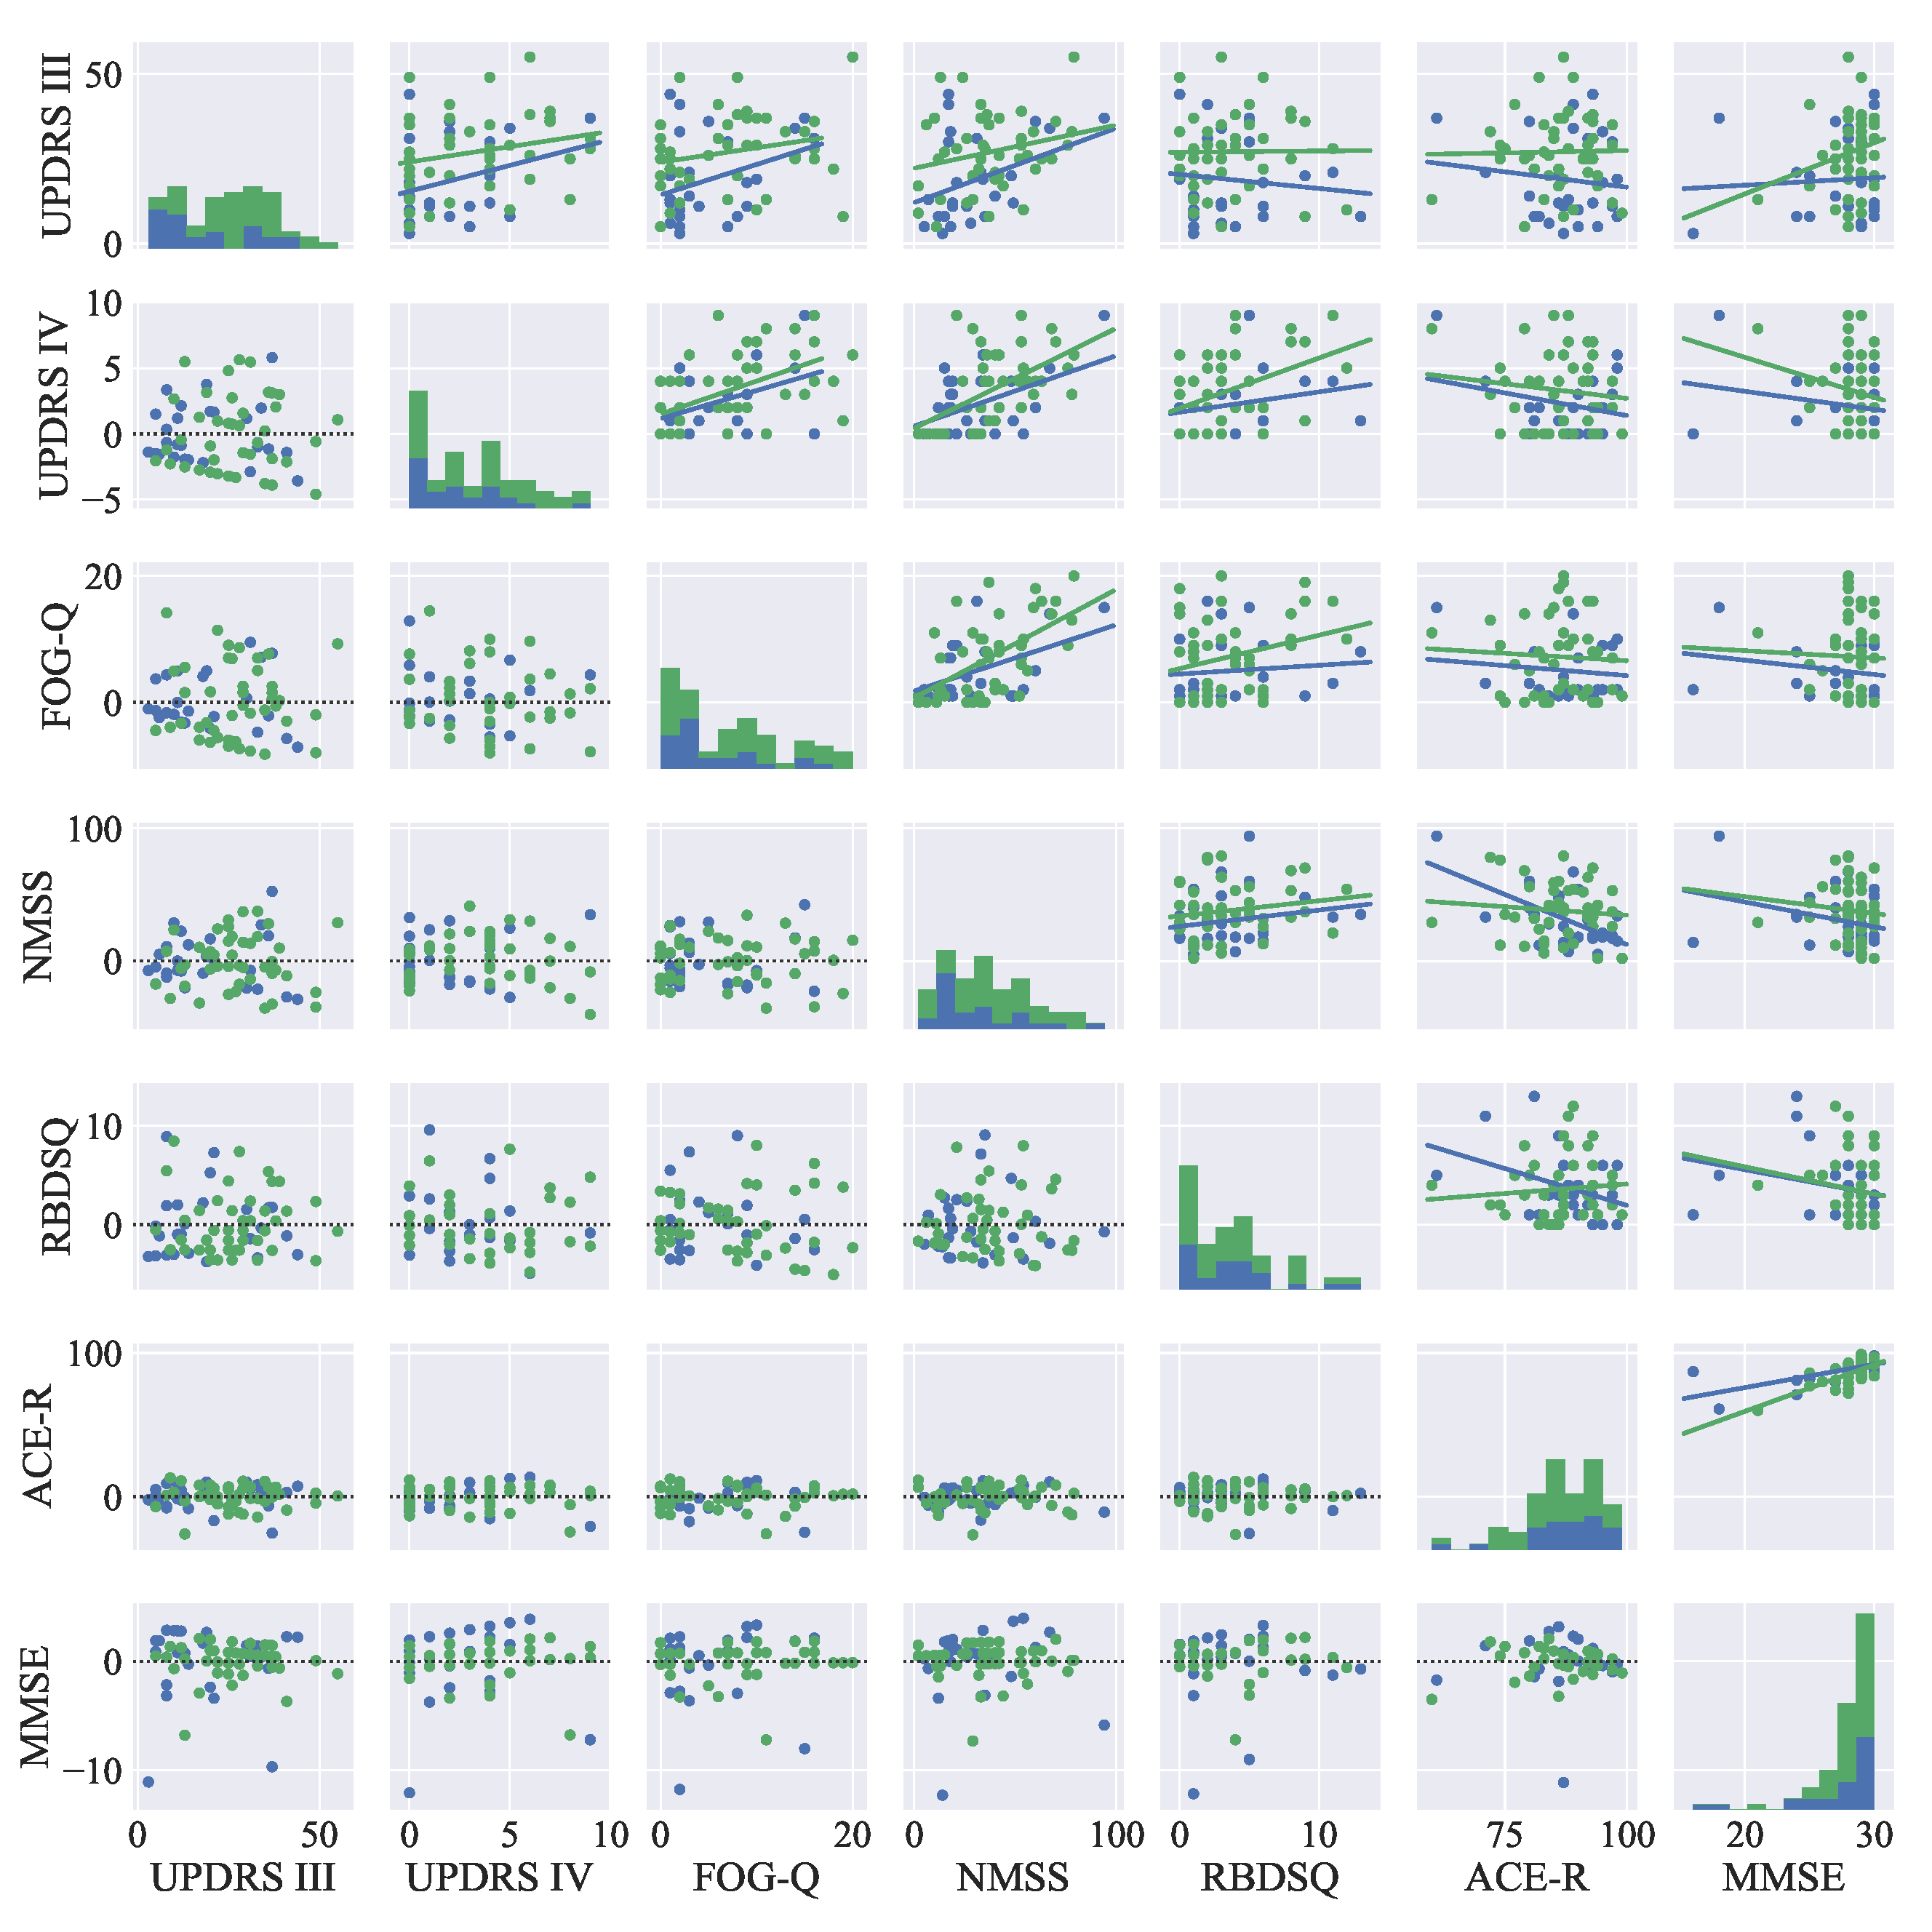
\includegraphics[width=0.99\textwidth]{pictures/ch5_clinical_statistics.eps}
	\caption[Descriptive statistical graphs of clinical data for PD patients.]{Descriptive statistical graphs of clinical characteristics of PD patients participated in this study: on the main diagonal, histograms are visualized. Next, the upper triangular part of the graph-grid shows scatter plots with the fitted lines of the linear regression models. And finally, the lower triangular part of the graph-grid is used to display residuals for the models shown in the the upper grid. Colour notation: blue colour represents female speakers, and green colour represents male speakers. For the description of the rating scales, see Table~\ref{tab:ch5_clinical_data}.}
	\label{fig:ch5_clinical_statistics}
\end{figure}

\subsection{Feature extraction}
\label{ch5_3_2}

As in the case of study presented in Chapter~\ref{ch4}, the following acoustic features quantifying dysprosody in HD were used~\cite{Brabenec2017}. To describe variation in pitch, fundamental frequency (F0) was used, specifically: standard deviation of F0 (FOSD), relative standard deviation of F0 (relF0SD), variation range of F0 (FOVR), and relative variation range of F0 (relF0VR) were computed. Regarding description of variation in intensity, squared energy operator (SEO) and Teager-Kaiser energy operator (TEO) were used, specifically: standard deviation of SEO/TEO (SEOSD/TEOSD), relative standard deviation of SEO/TEO (relSEOSD/relTEOSD), variation range of SEO/TEO (SEOVR/TEOVR), and relative variation range of SEO/TEO (relSEOVR/relTEOVR) were computed. And finally, total speech time (TST), net speech time (NST), total pause time (TPT), total speech rate (TSR), net speech rate (NSR), total pause time (pauses longer than $50$\,ms) (TPT\,($50$\,ms)), articulation rate (AR), and speech index of rhythmicity (SPIR) were computed to describe speech rate and pausing abnormalities.

\subsection{Analytical setup}
\label{ch5_3_3}

To describe the presence of possible relationship between the values of the computed acoustic features quantifying dysprosody in HD and other motor and non-motor symptoms (assessed by the selected clinical rating scales) in PD, Spearman's correlation coefficient ($\rho$) was used (short description of this method can be found in the previous chapter). The significance level of correlation ($p$) of $0.05$ was selected. Due to the limited number of samples and the exploratory character of the study, the correction for multiple comparisons was not performed. Moreover, due to the large number of clinical rating scales under focus, partial correlations were not computed to control for the effect of covariates, but rather classical correlations were applied to provide a~preliminary insight into association between dysprosody in HD and other non-speech symptoms of PD.

Consequently, multivariate regression models estimating values of the analysed clinical rating scales were built ($10$-fold cross-validation with $20$ repetitions was used for validation). However, as in the case of HD identification (see Chapter~\ref{ch4}), not all acoustic features were used for this purpose. As previously, a~modified version of sequential floating forward selection~\cite{Pohjalainen2014} algorithm was applied to reduce the number of features and create the regression models with low dimensionality, better clinical interpretability, and high performance~\cite{Guyon2006}. With respect to the actual regression algorithm, classification and regression trees (CART) were employed. Classification and regression trees are a~non-parametric supervised machine learning algorithm based on mathematical theory introduced in $1984$ by Breiman, Freidman, Olshen and Stone~\cite{Breiman1984} that are still commonly used in the field of biostatistics due to its robustness to outliers and ability to deal with highly dimensional and highly correlated data~\cite{Hastie2009}. The result of the algorithm are often well-interpretable, which makes this algorithm especially attractive.

To measure the prediction performance of the trained models, several conventional and widely-used regression metrics such as mean absolute error (MAE), and root mean squared error (RMSE) were employed. Moreover, a~novel regression metric named estimation error rate (EER) was computed to express the prediction error in percentage, which is particularly useful for easy and fast interpretation. These metrics are defined as:
\begin{eqnarray}
	\mathrm{MAE}  &=& \frac{1}{n}\sum_{i=1}^{n} \abs{y_{i}-\hat{y_{i}}}, \\
	\mathrm{RMSE} &=& \sqrt{\frac{1}{n}\sum_{i=1}^{n} (y_{i}-\hat{y_{i}})^2}, \\
	\mathrm{EER}  &=& \frac{1}{n \cdot r}\sum_{i=1}^{n} \abs{y_{i}-\hat{y_{i}}} \cdot 100\,[\%], 
\end{eqnarray}
where the above mentioned variables stands for: $n$ is the number of true/predicted values, $y_{i}$ and $\hat{y_{i}}$ represents the true and predicted values of the response variable, respectively, and $r$ denotes the range of values of the given clinical rating scale present in the dataset (this is particularly useful when interpreting the values of EER for the restricted range of values that is a~common situation when dealing with the data from patients with neurodegenerative disorders\footnote{It is important to note that every dataset is different in the participants. For instance, in the case of this study, patients with PD were acquired. These patients however are often in the moderate to severe stage of the disease since an accurate early PD diagnosis is rare or completely missing. Therefore, even though the clinical rating scales used to assess the parkinsonian manifestations are able to quantify very mild or severe disabilities, such data is almost never acquired. Hence, the conversion of some classical prediction metric such as mean absolute error into percentage can not simply be done using the range of the clinical rating scales because the resulting estimation error rates would be overestimating the performance of the trained models. For this reason, it is extremely important to consider the actual range of values present in the dataset.}, see Table~\ref{tab:ch5_clinical_data}). In the frame of this study, these regression metrics can be interpreted as: mean absolute error expresses the average absolute difference between the predicted and true values of the variable under focus, so that with higher mean absolute error, worse predictions are made. Root mean squared error expresses the square root of the average of squared prediction errors, so that with lower root mean squared error, even more inaccurate predictions are made. Furthermore, as opposed to RMSE, MAE has the advantage that it describes the prediction error in the same units as the variables themselves. However, RMSE is also frequently used because it amplifies larger differences and is therefore more sensitive to prediction errors. And finally, estimation error rate expresses the mean absolute error in relation to the range of values of the predicted variable, so that it gives the visual impression of the estimation error of the model given the actual statistical properties of the dataset.

\section{Results}
\label{ch5_4}

Results of the correlation analysis are summarized in Table~\ref{tab:ch5_statistical_analysis}. The table shows top three acoustic features sorted according to their significance level of correlation expressed by Spearman's correlation coefficient. The following results showing the correlation for the specific prosodic areas under focus were achieved\footnote{Only a~single statistically significant feature per prosodic area is presented, therefore it might happen that some features will not appear in the summary. Features with $p>0.05$ are not shown as well as they are considered statistically insignificant. For complete picture, see~\ref{tab:ch5_statistical_analysis}} (* means that $p<0.05$; ** means that $p<0.01$; T1\,--\,poem recitation task; T2\,--\, reading with neutral emotion; and T3\,--\,stress-modified reading):
\begin{enumerate}
	\item UPDRS~III\,--\,the strongest correlation was found in the case of features describing reduced variation in pitch and intensity of speech in all three speech tasks (T1--T3) (T1: $-0.38^{**}$ (F0VR), $-0.30^{**}$ (TEOSD); T2: $-0.28^{*}$ (F0SD), $0.28^{*}$ (SEOSD); and T3: $-0.37^{**}$ (F0VR), $-0.30^{*}$ (TEOVR)).
	\item UPDRS~IV\,--\,the strongest correlation was found in the case of features describing reduced variation in intonation (T1, T2), intensity of speech (T3), and speech rate abnormalities (T1, T2) (T1: $0.29^{*}$ (relF0SD), $0.21^{*}$ (TPT\,(50\,ms)); T2: $0.32^{**}$ (relF0SD), $0.31^{**}$ (TPT\,(50\,ms)); and T3: $-0.21^{*}$ (TEOSD), $-0.21^{*}$ (F0VR)).
	\item FOG-Q\,--\,the strongest correlation was found mostly in the case of features describing speech rate abnormalities in all three speech tasks (T1--T3), and reduced variation in intensity of speech (T1) (T1: $-0.35^{**}$ (NST), $0.28^{*}$ (relF0SD); T2: $0.42^{**}$ (TPT\,(50\,ms)); and T3: $-0.27^{*}$ (NST)).
	\item NMSS\,--\,the strongest correlation was found in the case of features describing reduced variation in intonation and intensity of speech in all three speech tasks (T1--T3) (T1: $-0.29^{*}$ (TEOSD), $0.26^{*}$ (relF0SD); T2: $0.36^{*}$ (relF0SD), $0.31^{*}$ (relTEOVR); and T3: $-0.36^{*}$ (TEOVR), $-0.29^{*}$ (F0VR)).
	\item RBDSQ\,--\,the strongest correlation was found only in the case of features describing reduced variation in intensity of speech (T1, T2) (T1: $0.20^{*}$ (TEOSD); and T2: $-0.23^{*}$ (SEOSD)).
	\item ACE-R\,--\,the strongest correlation was found in the case of features describing speech rate abnormalities (T1), and reduced variation in intensity of speech (T3) (T1: $-0.43^{*}$ (TPT); T3: $0.23^{*}$ (TEOSD)).
	\item MMSE\,--\,the strongest correlation was found in the case of a~single feature describing speech rate abnormalities (T1: $-0.26^{*}$ (TPT)).
	\item BDI\,--\,none of the features showed statistically significant correlation.
\end{enumerate}

\begin{table*}[htb!]
	\centering
	\begin{threeparttable}
		\caption{Correlation analysis of the prosodic features.}
		\label{tab:ch5_statistical_analysis}
		\footnotesize
		\centering
		\begin{tabular}{l l r c l r c l r c}

			\hline\hline\noalign{\smallskip}
			\rowcolor{gray_table}
			& \multicolumn{3}{c}{T1} & \multicolumn{3}{c}{T2} & \multicolumn{3}{c}{T3} \\
			\noalign{\smallskip}
			scale & features & $\rho$ & $p$ & features & $\rho$ & $p$ & features & $\rho$ & $p$ \\
			\noalign{\smallskip}\hline\noalign{\smallskip}
			
			\multirow{3}{*}{UPDRS~III} 
			& F0VR  & -0.38 & ** & F0SD  & -0.28 & *  & F0VR  & -0.37 & ** \\
			& TEOSD & -0.30 & ** & SEOSD &  0.28 & *  & F0SD  & -0.34 & ** \\
			& TEOVR & -0.25 & *  & SEOVR &  0.28 & *  & TEOVR & -0.30 & *  \\
			
			\noalign{\smallskip}
			\multirow{3}{*}{UPDRS~IV} 
			& relF0SD       &  0.29 & *  & relF0SD       &  0.32 & ** & TEOSD & -0.21 & *  \\
			& TPT\,(50\,ms) &  0.21 & *  & TPT\,(50\,ms) &  0.31 & ** & F0VR  & -0.21 & *  \\
			& relF0VR       &  0.20 &    & AR            & -0.31 & ** & TEOVR & -0.18 &    \\
			
			\noalign{\smallskip}
			\multirow{3}{*}{FOG-Q} 
			& NST     & -0.35 & ** & TPT\,(50\,ms) &  0.42 & ** & NST & -0.27 & *  \\
			& NSR     &  0.35 & ** & AR            & -0.42 & ** & NSR &  0.27 & *  \\
			& relF0SD &  0.28 & *  & NST           & -0.41 & ** & TST & -0.26 & *  \\
			
			\noalign{\smallskip}
			\multirow{3}{*}{NMSS} 
			& TEOSD   & -0.29 & *  & relF0SD  &  0.36 & ** & TEOVR & -0.36 & ** \\
			& relF0SD &  0.26 & *  & relTEOVR &  0.31 & ** & TEOSD & -0.35 & ** \\
			& TPT     &  0.20 &    & relF0VR  &  0.26 & *  & F0VR  & -0.29 & *  \\
			
			\noalign{\smallskip}
			\multirow{3}{*}{RBDSQ} 
			& TEOSD &  0.20 & *  & SEOSD    & -0.23 & *  & SPIR    & -0.18 &    \\
			& TEOVR &  0.20 &    & relSEOVR &  0.10 &    & TEOSD   &  0.17 &    \\
			& SEOSD & -0.17 &    & SEOVR    & -0.09 &    & relF0SD &  0.17 &    \\
			
			\noalign{\smallskip}
			\multirow{3}{*}{ACE-R} 
			& TPT & -0.43 & ** & TEOSD    &  0.18 &    & TEOSD &  0.23 & *  \\
			& TST & -0.33 & ** & relSEOVR &  0.16 &    & TEOVR &  0.20 &    \\
			& TSR &  0.33 & ** & relF0VR  & -0.16 &    & SPIR  &  0.20 &    \\
			
			\noalign{\smallskip}
			\multirow{3}{*}{MMSE} 
			& TPT      & -0.26 & *  & relTEOVR & -0.17 &    & F0SD          & -0.18 &    \\
			& relSEOSD & -0.17 &    & NST      &  0.16 &    & SEOVR         & -0.13 &    \\
			& TST      & -0.16 &    & TPT      & -0.16 &    & TPT\,(50\,ms) & -0.12 &    \\
			
			\noalign{\smallskip}
			\multirow{3}{*}{BDI} 
			& relTEOVR &  0.18 &    & SEOSD    &  0.21 &    & relTEOSD &  0.18 &    \\
			& SEOSD    &  0.16 &    & relTEOVR &  0.15 &    & relSEOSD & -0.18 &    \\
			& relTEOSD &  0.15 &    & relSEOVR & -0.14 &    & relSEOVR & -0.16 &    \\
			
			\noalign{\smallskip}\hline\hline
		\end{tabular}
		
		\begin{tablenotes}
			\scriptsize
			\item[1] Table notation: T1\,--\,poem recitation task; T2\,--\,emotionally-neutral reading task; T3\,--\,stress-modified reading task; $\rho$~--~Spearman's correlation coefficient; $p$~--~significance level of correlation (* means $p<0.05$; ** means $p<0.01$); UPDRS~III\,--\,Unified Parkinson's disease rating scale, part~III: evaluation of motor function~\cite{Fahn1987}; UPDRS~IV\,--\,Unified Parkinson's disease rating scale, part~IV: evaluation of complications of therapy (Hoehn and Yahr scale, staging of severity of Parkinson's disease)~\cite{Fahn1987}; FOG-Q\,--\,Freezing of gait questionnaire~\cite{Giladi2000}; NMSS\,--\,Non-motor symptoms scale~\cite{Chaudhuri2007}; RBDSQ\,--\,The REM sleep behavior disorder screening questionnaire~\cite{Stiasny2007}; ACE-R\,--\,Addenbrooke's cognitive examination-revised~\cite{Larner2007}; MMSE\,--\,Mini-mental state examination~\cite{Folstein1975}; BDI\,--\,Beck depression inventory \cite{Beck2000, Beck1961}.
		\end{tablenotes}	
	\end{threeparttable}
\end{table*}

Moreover, three specific clinical rating scales were selected: UPDRS~III (evaluation of motor deficits), FOG-Q (evaluation of gait freezing), ACE-R (evaluation of cognitive deficits). For these three scales, regression plots can be seen in Figure~\ref{fig:ch5_correlation_plots}. The figure provides a~visual impression about the strength of a~linear relationship between the most correlated acoustic features and the values of the selected clinical rating scales (a~single feature is chosen for each scenario). 

\begin{figure}[htb!]
	\centering
	\scriptsize
	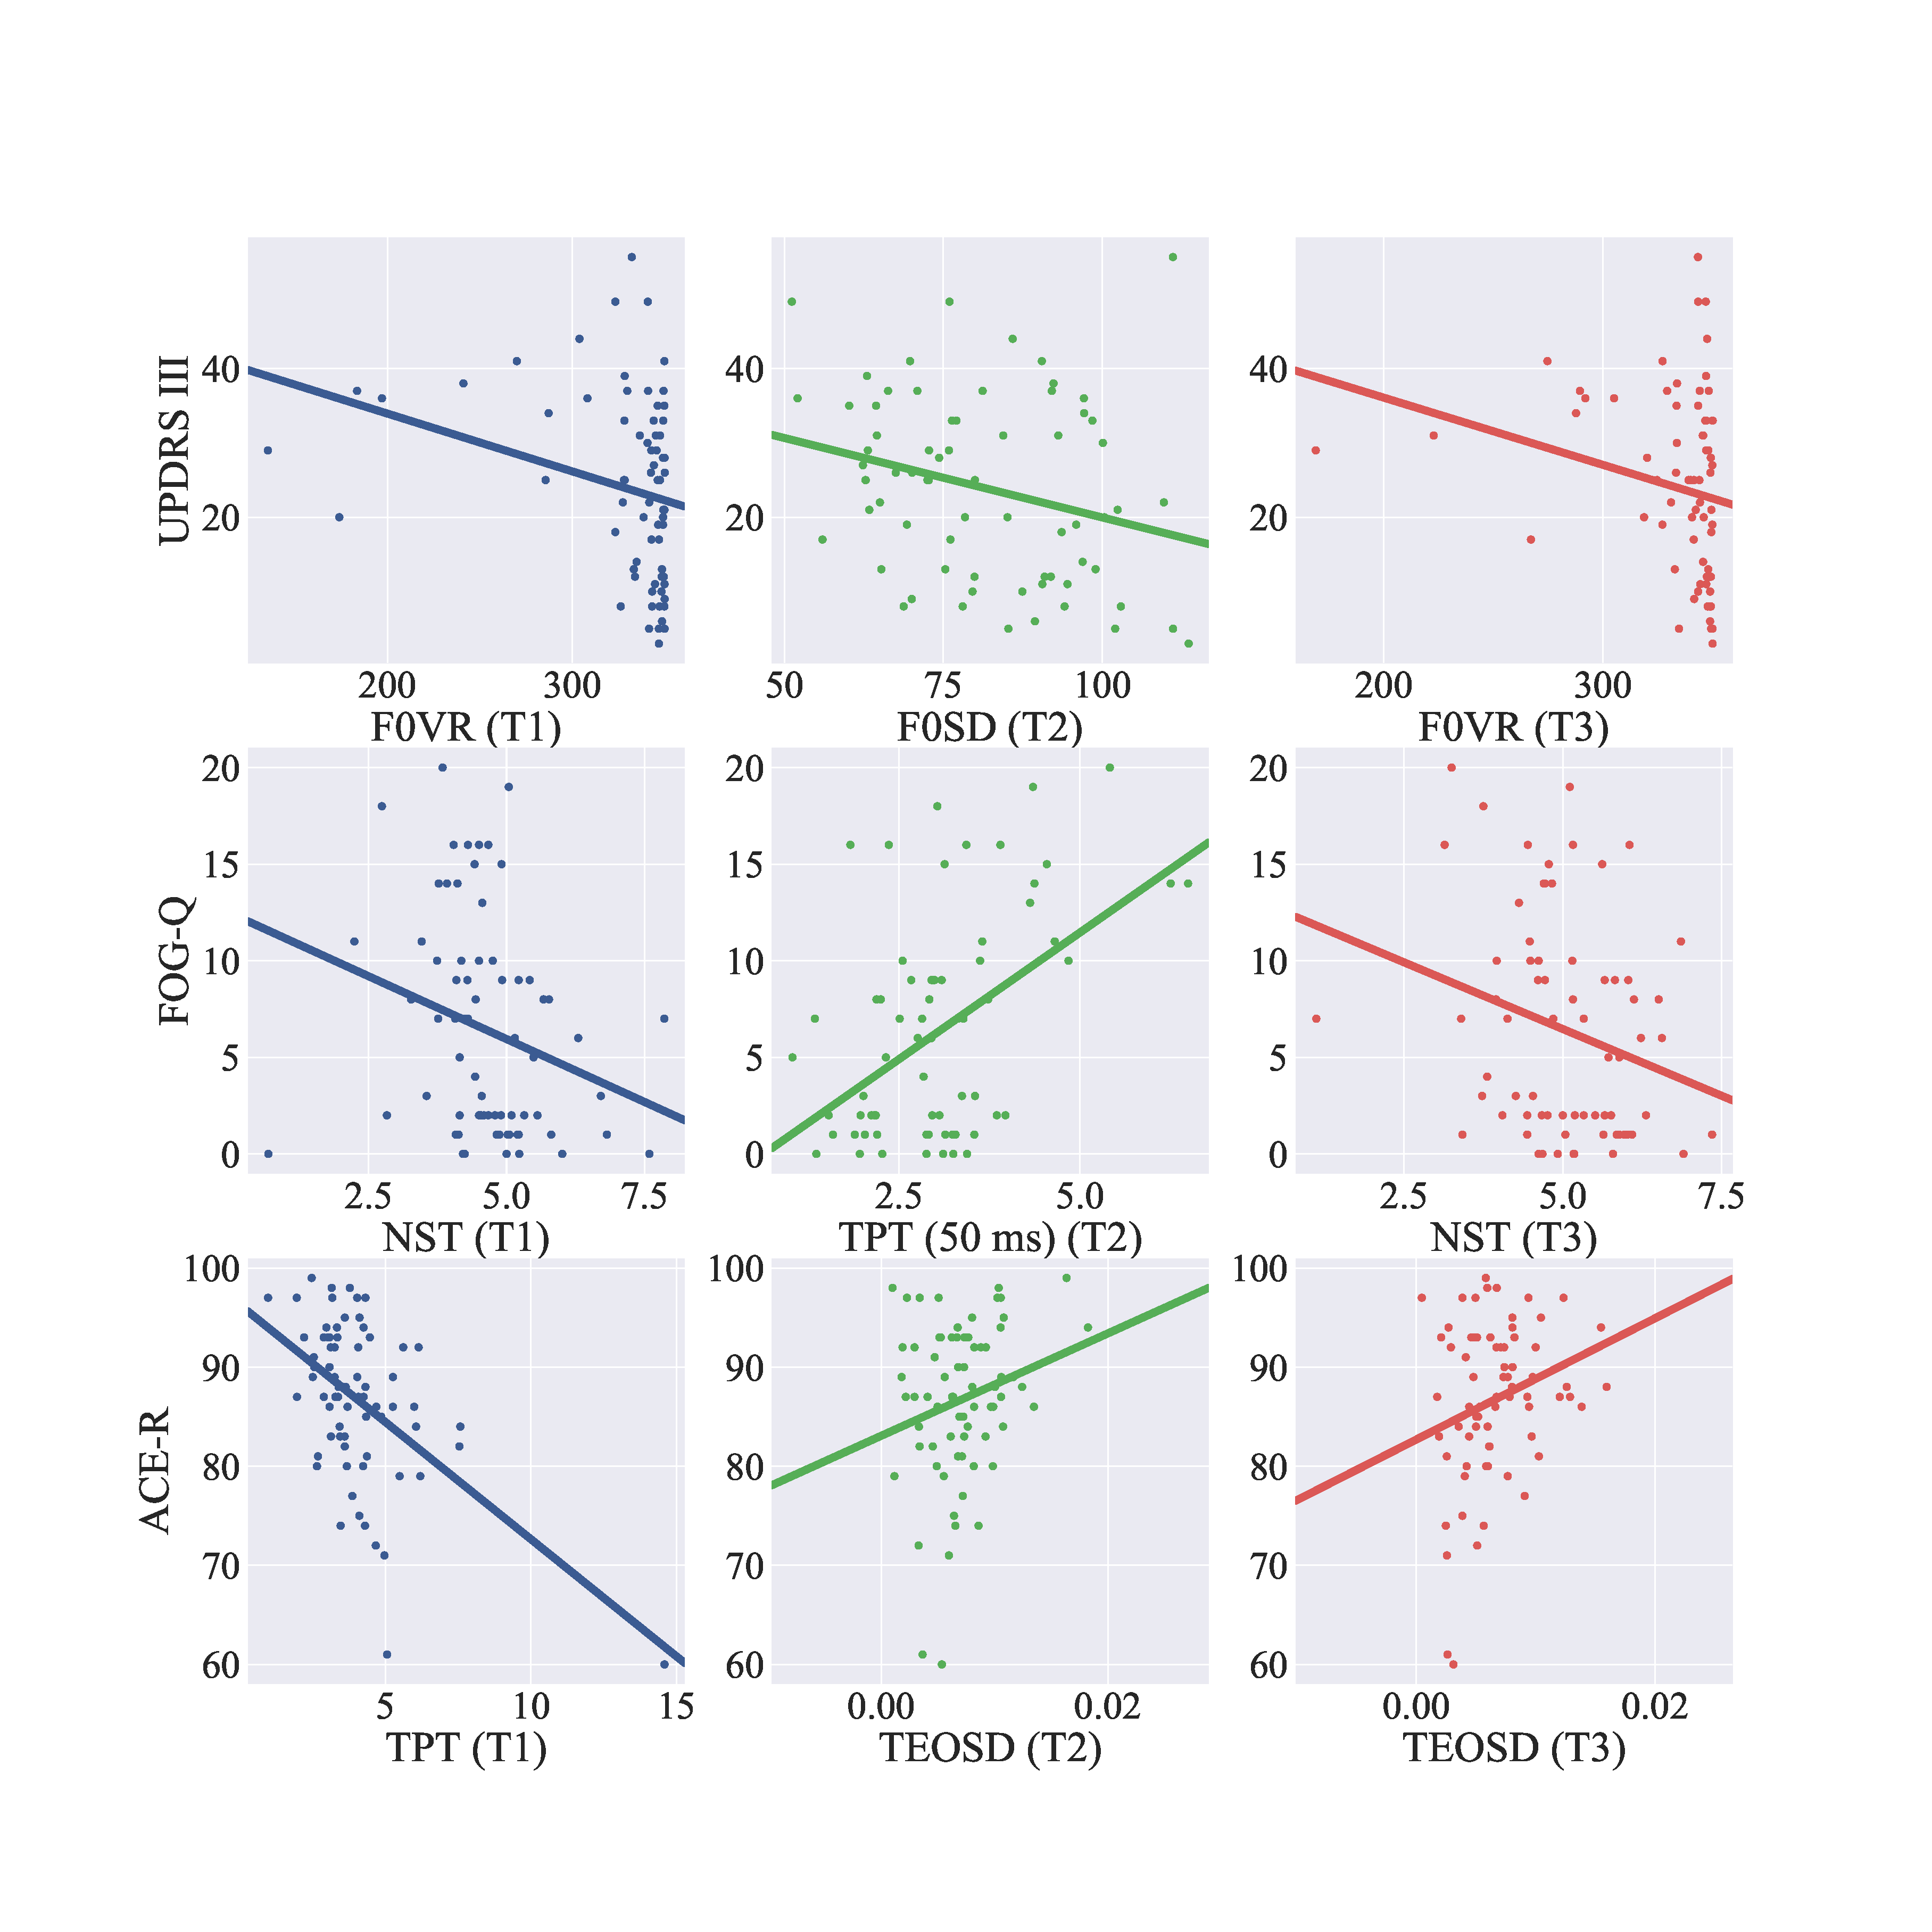
\includegraphics[width=0.99\textwidth]{pictures/ch5_correlation_plots.eps}
	\caption[Regression plots for UPDRS~III, FOG-Q, and ACE-R.]{Regression plots (scatter plots with the fitted line of the robust linear regression estimator) of the selected rating scales (UPDRS~III, FOG-Q, ACE-R) for all three speech tasks performed by all PD patients: T1\,--\,poem recitation task (first column/blue colour); T2\,--\,emotionally-neutral reading (second column/green colour); and T3\,--\,stress-modified reading (third column/red colour). Only one feature for each clinical rating scale/speech feature is visualized (selected according to the Spearman's correlation coefficient, see Table~\ref{tab:ch5_statistical_analysis}). For more information about the acoustic features notation, see Section~\ref{ch5_3_2}.}
	\label{fig:ch5_correlation_plots}
\end{figure}

As can be seen, the strong relationship between reduced variation in pitch and UPDRS~III (in the case of all the three speech tasks) is evident. Specifically, the flatter the intonation, the more severe motor disability assessed by UPDRS~III can be observed. Next, the strong relationship between speech rate/pausing abnormalities and FOG-Q (in the case of all the three speech tasks) is present as well. Specifically, the faster the speech during poem recitation, larger number of pauses (longer that $50$\,ms) during emotionally-neutral reading, and faster the speech during stress-modified reading, the more severe gait freezing episodes assessed by UPDRS~III can be observed. And finally, the strong relationship between speech rate/pausing abnormalities and ACE-R in the case of poem recitation can be seen. For the other two tasks, the association is much weaker (less statistically significant as well). Specifically, the faster speech (less time spent on pausing) during poem recitation, and larger deviation of speech intensity during reading (emotionally-neutral, and stress-modified), the more severe cognitive deficits assessed by ACE-R can be observed. These observations emphasize the fact that poem recitation task is a~great candidate to emphasize monopitch in HD, but also some cognitive deficits that are probably related to worse control of speech tempo (patients try to compensate it by occasional rushes of speech, etc.).

Next, for UPDRS~III, FOG-Q, and ACE-R, multivariate regression models using the features selected by the feature selection algorithm, were built and visualized (visualization of the approximation of decision making performed by the regression tree) using the three graphs, see Figure~\ref{fig:ch5_regression_tree_updrs}, Figure~\ref{fig:ch5_regression_tree_fogq}, and Figure~\ref{fig:ch5_regression_tree_acer}, respectively. Moreover, the results of the multivariate regression analysis are summarized in Table~\ref{tab:ch5_classification_groups}, and Table~\ref{tab:ch5_classification_combination}.

\begin{figure}[htb!]
	\centering
	\scriptsize
	\includegraphics[width=0.99\textwidth]{pictures/ch5_tree_model_updrs.pdf}
	\caption[Regression tree graph visualization for UPDRS~III]{Visualization of the regression tree built to estimate UPDRS~III. The tree was trained using a~single training run applied on all data in the dataset/selected features (hence the decision making of the tree is an approximation of the behavior responsible for the results summarized in Table~\ref{tab:ch5_classification_combination}). In the case of this tree: TST (T2), F0VR (T1), and TEOSD (T1) were used. For explanation of the speech task and acoustic feature notation, see Section~\ref{ch5_3_1}, and Section~\ref{ch5_3_2}, respectively.}
	\label{fig:ch5_regression_tree_updrs}
\end{figure}

\begin{figure}[htb!]
	\centering
	\scriptsize
	\includegraphics[width=0.60\textwidth]{pictures/ch5_tree_model_fogq.pdf}
	\caption[Regression tree graph visualization for FOG-Q]{Visualization of the regression tree built to estimate FOG-Q. The tree was trained using a~single training run applied on all data in the dataset/selected features (hence the decision making of the tree is an approximation of the behavior responsible for the results summarized in Table~\ref{tab:ch5_classification_combination}). In the case of this tree: TPT (T2), F0VR (T1), and SEOVR (T1) were used. For explanation of the speech task and acoustic feature notation, see Section~\ref{ch5_3_1}, and Section~\ref{ch5_3_2}, respectively.}
	\label{fig:ch5_regression_tree_fogq}
\end{figure}

\begin{figure}[htb!]
	\centering
	\scriptsize
	\includegraphics[width=0.60\textwidth]{pictures/ch5_tree_model_acer.pdf}
	\caption[Regression tree graph visualization for ACE-R]{Visualization of the regression tree built to estimate ACE-R. The tree was trained using a~single training run applied on all data in the dataset/selected features (hence the decision making of the tree is an approximation of the behavior responsible for the results summarized in Table~\ref{tab:ch5_classification_combination}). In the case of this tree: TPT (T2), and relSEOSD (T1) were used. For explanation of the speech task and acoustic feature notation, see Section~\ref{ch5_3_1}, and Section~\ref{ch5_3_2}, respectively.}
	\label{fig:ch5_regression_tree_acer}
\end{figure}

\begin{table*}[htb!]
	\centering
	\begin{threeparttable}
		\caption{Results of the regression analysis for individual speech tasks.}
		\label{tab:ch5_classification_groups}
		\footnotesize
		\centering
		\begin{tabular}{l c c c c l}
		
			\hline\hline\noalign{\smallskip}
			\rowcolor{gray_table}
			scale & MAE & RMSE & EER & No. & selected features \\
			\noalign{\smallskip}
			\multicolumn{6}{c}{Poem recitation task} \\
			\noalign{\smallskip}\hline\noalign{\smallskip}
			
			UPDRS III &  9.41~$\pm$~2.73 & 11.45~$\pm$~3.13 & 18.11~$\pm$~5.26 & 2 & F0VR, TEOSD \\
			UPDRS IV  &  2.12~$\pm$~0.65 &  2.69~$\pm$~0.72 & 23.65~$\pm$~7.26 & 1 & relTEOVR \\
			FOG-Q     &  4.52~$\pm$~1.57 &  5.83~$\pm$~1.92 & 22.61~$\pm$~7.89 & 3 & TEOVR, F0VR, TST \\
			NMSS      & 18.55~$\pm$~4.48 & 21.88~$\pm$~4.83 & 20.16~$\pm$~4.87 & 1 & relTEOVR \\
			RBDSQ     &  2.86~$\pm$~0.80 &  3.50~$\pm$~0.94 & 22.06~$\pm$~6.17 & 1 & relSEOVR \\
			ACE-R     &  6.18~$\pm$~1.84 &  7.67~$\pm$~2.23 & 15.86~$\pm$~4.72 & 1 & relSEOSD \\
			MMSE      &  1.83~$\pm$~0.77 &  2.52~$\pm$~1.26 & 13.13~$\pm$~5.50 & 2 & SEOVR, TPT \\
			BDI       &  5.65~$\pm$~1.52 &  6.68~$\pm$~1.80 & 20.94~$\pm$~5.63 & 2 & TPT, relSEOVR \\
			
			\noalign{\smallskip}\hline\noalign{\smallskip}
			\multicolumn{6}{c}{Reading with neutral emotion} \\
			\noalign{\smallskip}\hline\noalign{\smallskip}
			
			UPDRS III & 10.44~$\pm$~2.46 & 12.12~$\pm$~2.63 & 20.08~$\pm$~4.74 & 1 & TPT \\
			UPDRS IV  &  2.31 $\pm$~0.50 &  2.66~$\pm$~0.55 & 25.76~$\pm$~5.63 & 1 & TPT \\
			FOG-Q     &  3.86~$\pm$~1.22 &  4.80~$\pm$~1.42 & 19.31~$\pm$~6.14 & 3 & relF0VR, TPT, NSR \\
			NMSS      & 14.51~$\pm$~4.29 & 17.78~$\pm$~4.98 & 15.78~$\pm$~4.66 & 3 & TPT, relF0SD, TEOSD \\
			RBDSQ     &  2.51~$\pm$~0.68 &  3.04~$\pm$~0.89 & 19.38~$\pm$~5.24 & 1 & TPT \\
			ACE-R     &  6.80~$\pm$~2.12 &  8.34~$\pm$~2.66 & 17.44~$\pm$~5.45 & 1 & TPT \\
			MMSE      &  1.61~$\pm$~0.68 &  2.25~$\pm$~1.24 & 11.50~$\pm$~4.87 & 1 & TPT \\
			BDI       &  4.92~$\pm$~1.39 &  6.00~$\pm$~1.66 & 18.22~$\pm$~5.18 & 1 & TPT \\
			
			\noalign{\smallskip}\hline\noalign{\smallskip}
			\multicolumn{6}{c}{Stress-modified reading} \\
			\noalign{\smallskip}\hline\noalign{\smallskip}
			
			UPDRS III & 10.50~$\pm$~3.23 & 13.10~$\pm$~4.01 & 20.20~$\pm$~6.22 & 2 & relTEOSD, F0SD \\
			UPDRS IV  &  2.45~$\pm$~0.64 &  2.99~$\pm$~0.67 & 27.27~$\pm$~7.16 & 4 & SEOVR, F0VR, AR, TPT \\
			FOG-Q     &  4.90~$\pm$~1.29 &  5.78~$\pm$~1.44 & 24.50~$\pm$~6.47 & 2 & TSR, TST \\
			NMSS      & 17.29~$\pm$~4.88 & 20.91~$\pm$~5.67 & 18.80~$\pm$~5.31 & 1 & TEOVR \\
			RBDSQ     &  2.64~$\pm$~0.71 &  3.23~$\pm$~0.80 & 20.33~$\pm$~5.49 & 2 & TEOSD, F0VR \\
			ACE-R     &  6.18~$\pm$~1.84 &  7.67~$\pm$~2.23 & 15.86~$\pm$~4.72 & 3 & TST, TSR, relSEOSD \\
			MMSE      &  1.76~$\pm$~0.67 &  2.36~$\pm$~1.12 & 12.62~$\pm$~4.83 & 1 & TST \\
			BDI       &  5.44~$\pm$~1.63 &  6.72~$\pm$~1.81 & 20.15~$\pm$~6.04 & 3 & TEOVR, F0VR, SEOSD \\
			
			\noalign{\smallskip}\hline\hline
		\end{tabular}
		
		\begin{tablenotes}
		\scriptsize
			\item[1] Table notation: MAE\,--\,mean absolute error; RMSE\,--\,root mean squared error; EER\,--\,relative estimation error rate (MAE divided by the range of actual values of clinical rating scale present in the dataset; expressed in $\%$); No.\,--\,number of selected features; UPDRS~III\,--\,Unified Parkinson's disease rating scale, part~III: evaluation of motor function~\cite{Fahn1987}; UPDRS~IV\,--\,Unified Parkinson's disease rating scale, part~IV: evaluation of complications of therapy (Hoehn and Yahr scale, staging of severity of Parkinson's disease)~\cite{Fahn1987}; FOG-Q\,--\,Freezing of gait questionnaire~\cite{Giladi2000}; NMSS\,--\,Non-motor symptoms scale~\cite{Chaudhuri2007}; RBDSQ\,--\,The REM sleep behavior disorder screening questionnaire~\cite{Stiasny2007}; ACE-R\,--\,Addenbrooke's cognitive examination-revised~\cite{Larner2007}; MMSE\,--\,Mini-mental state examination~\cite{Folstein1975}; BDI\,--\,Beck depression inventory \cite{Beck2000, Beck1961}.
		\end{tablenotes}
	\end{threeparttable}
\end{table*}

\begin{table*}[htb!]
	\centering
	\begin{threeparttable}
		\caption{Results of the regression analysis for a~combination of speech tasks.}
		\label{tab:ch5_classification_combination}
		\footnotesize
		\centering
		\begin{tabular}{l c c c c l}
		
			\hline\hline\noalign{\smallskip}
			\rowcolor{gray_table}
			scale & MAE & RMSE & EER & No. & selected features \\
			\noalign{\smallskip}\hline\noalign{\smallskip}
			
			UPDRS III &  9.10~$\pm$~2.93 & 11.27~$\pm$~3.46 & 17.52~$\pm$~5.64 & 3 & TST$^{2}$, F0VR$^{1}$, TEOSD$^{1}$ \\
			UPDRS IV  &  2.31~$\pm$~0.50 &  2.65~$\pm$~0.56 & 25.75~$\pm$~5.64 & 1 & TPT$^{2}$ \\
			FOG-Q     &  3.45~$\pm$~1.28 &  4.54~$\pm$~1.61 & 17.28~$\pm$~6.42 & 3 & TPT$^{2}$, F0VR$^{1}$, SEOVR$^{1}$ \\
			NMSS      & 17.03~$\pm$~4.35 & 20.50~$\pm$~4.86 & 18.52~$\pm$~4.73 & 1 & TPT$^{2}$ \\
			RBDSQ     &  2.26~$\pm$~0.83 &  2.88~$\pm$~1.03 & 17.44~$\pm$~6.40 & 3 & F0SD$^{1}$, SEOSD$^{1}$, TPT$^{2}$ \\
			ACE-R     &  6.20~$\pm$~1.85 &  7.68~$\pm$~2.22 & 15.72~$\pm$~4.75 & 2 & TPT$^{2}$, relSEOSD$^{1}$ \\
			MMSE      &  1.60~$\pm$~0.68 &  2.25~$\pm$~1.24 & 11.49~$\pm$~4.92 & 1 & TPT$^{2}$ \\
			BDI       &  4.91~$\pm$~1.40 &  6.00~$\pm$~1.66 & 18.21~$\pm$~5.21 & 1 & TPT$^{2}$ \\
			
			\noalign{\smallskip}\hline\hline
		\end{tabular}
		
		\begin{tablenotes}
		\scriptsize
			\item[1] Table notation: $^{1}$\,--\,poem recitation task; $^{2}$\,--\,reading with neutral emotion; $^{3}$\,--\,stress-modified reading task; MAE\,--\,mean absolute error; RMSE\,--\,root mean squared error; EER\,--\,relative estimation error rate (mean absolute error divided by the range of actual values of clinical rating scale present in the dataset; expressed in $\%$); No.\,--\,number of selected features; UPDRS~III\,--\,Unified Parkinson's disease rating scale, part~III: evaluation of motor function~\cite{Fahn1987}; UPDRS~IV\,--\,Unified Parkinson's disease rating scale, part~IV: evaluation of complications of therapy (Hoehn and Yahr scale, staging of severity of Parkinson's disease)~\cite{Fahn1987}; FOG-Q\,--\,Freezing of gait questionnaire~\cite{Giladi2000}; NMSS\,--\,Non-motor symptoms scale~\cite{Chaudhuri2007}; RBDSQ\,--\,The REM sleep behavior disorder screening questionnaire~\cite{Stiasny2007}; ACE-R\,--\,Addenbrooke's cognitive examination-revised~\cite{Larner2007}; MMSE\,--\,Mini-mental state examination~\cite{Folstein1975}; BDI\,--\,Beck depression inventory \cite{Beck2000, Beck1961}.
		\end{tablenotes}
	\end{threeparttable}
\end{table*}

With respect to the separate analysis (analysis of the speech tasks separately in direction of evaluating their sufficiency to assess severity of PD by estimating the clinical rating scales that are used to assess motor and non-motor deficits occurring with this disease), the following results were achieved: a) T1\,--\,most of the selected acoustic features are based on the description of reduced variability in intonation and intensity of speech. The lowest estimation error rate was obtained in the case of MMSE (SEOVR, TPT): $\mbox{EER}=13.13~\pm~5.50\,\%$, closely followed by ACE-R (relSEOSD): $\mbox{EER}=15.86~\pm~4.72$, and UPDRS~III (F0VR, TEOSD): $\mbox{EER}=18.11~\pm~5.26\,\%$; b) T2\,--\,in $6$ out of the total number of $8$ analysed clinical rating scales, the feature selection found only a~single feature based on the description of speech rate and pausing abnormalities (TPT) to be sufficient enough to describe the relationship between dysprosody in HD and severity of PD. The lowest estimation error rate was obtained in the case of MMSE (TPT): $\mbox{EER}=11.50~\pm~4.87\,\%$; and c) T3\,--\,features based on the description of reduced variability of intensity of speech and speech rate abnormalities dominated most of the models. The lowest estimation error rate was obtained in the case of MMSE (TST): $\mbox{EER}=12.62~\pm~4.83\,\%$, closely followed by ACE-R (TST, TSR, relSEOSD): $\mbox{EER}=15.86~\pm~4.72\,\%$, and NMSS (TEOVR): $\mbox{EER}=18.80~\pm~5.31\,\%$.

Regarding the combined analysis (analysis of the combination of the speech tasks in direction of evaluating the power of the combined model to robustly and complexly assess severity of PD), combination of the speech tasks resulted into lower estimation error rates in most of the cases in which more than a~single acoustic feature was selected. The prediction power of the regression models was slightly improved in the following clinical rating scales (improvements are expressed in \%): $\mbox{UPDRS~III}=0.59\,\%$, $\mbox{FOG-Q}=2.04\,\%$, $\mbox{RBDSQ}=1.94\,\%$. However, as can be seen, in most of the cases, a~single prosodic feature seems to be sufficiently describing a~relationship between dysprosody in HD and other non-speech symptoms occurring with PD. Hypothetically, the prediction power of these models could be increased when taking other HD manifestations into account. Nevertheless, the results clearly show dysprosody is related with other motor (as assessed by UPDRS~III, or FOG-Q) and non-motor (as assessed by MMSE or ACE-R) symptoms in PD.

\section{Conclusion}
\label{ch5_5}

Up to this day, several world-renown researchers analysed relationship between speech disorders in HD and other non-speech symptoms of PD \cite{Goberman2005b, Moreau2007, Skodda2009, Skodda2011c, Skodda2013}. However, investigation of the association between acoustic features quantifying dysprosody in HD and a~complex set of clinical rating scales assessing motor and non-motor symptoms of PD is still rare or missing. This study therefore provides further analysis of the relationship between HD and other aspects of PD using the correlation analysis. Regarding the results, the following conclusion can be made.

Concerning UPDRS~III~\cite{Fahn1987}, the strongest correlation can be observed for the acoustic features describing reduced variation in intonation and intensity of speech. Specifically, in the case of poem recitation task, reduced variation in fundamental frequency was found correlated with higher severity of motor symptoms (F0VR: $-0.38$, $p<0.01$) present in PD, which highlights and confirms the previous findings proposed in Chapter~\ref{ch4} reporting that when PD patients are exposed to additional rhythmical demands, the prosodic deficits occurring with HD gets emphasized. This phenomenon can also be found in the case of stress-modified reading (F0VR: $-0.37$, $p<0.01$) confirming the relevancy of this speech task as well. On top of that, smaller variation and standard deviation of speech intensity was also found correlated with the higher severity of PD for both emotionally-neutral reading (TEOSD: $-0.30$, $p<0.01$) and stress-modified reading (TEOVR: $-0.30$, $p<0.05$). Regarding UPDRS~IV~\cite{Fahn1987}, the strongest correlation can be observed for the acoustic features describing reduced variation in intonation, and speech rate/pausing abnormalities. Interestingly, the best results were achieved for the emotionally-neutral reading task. Specifically, larger standard deviation of fundamental frequency (relF0SD: $0.32$, $p<0.01$), larger number of pauses longer than 50\,ms (TPT\,(50\,ms): $0.31$, $p<0.01$), and slow rate of speech (AR: $-0.31$, $p<0.01$) were found correlated with higher severity of PD. With respect to FOG-Q~\cite{Giladi2000}, the strongest correlation can be observed almost exclusively for the features describing speech rate/pausing abnormalities, which suggests that the relationship between HD and freezing of gait in PD is independent of stress and rhythm. Specifically, larger number of pauses longer than 50\,ms (TPT\,(50\,ms): $0.42$, $p<0.01$), and slow rate of speech (AR: $-0.42$, $p<0.01$) were found correlated with the higher severity of gait freezing in PD. Additionally, statistically significant correlations are present for poem recitation (NST: $-0.35$, $p<0.01$) and stress-modified reading (NST: $-0.27$, $p<0.05$) as well. These results confirm the relationship between the freezing of gait and speech rate disturbances in HD reported by Park et al.~\cite{Park2014} in $2014$. Regarding NMSS~\cite{Chaudhuri2007}, the strongest correlation can be observed for the acoustic features describing reduced variation in intonation and intensity of speech. These acoustic features dominated in the case of all the three speech tasks. Specifically, larger standard deviation of fundamental frequency (relTEOVR: $0.36$, $p<0.01$) and variation in speech intensity (relTEOVR: $0.31$, $p<0.01$) during emotionally-neutral reading, and smaller variation (relTEOVR: $-0.36$, $p<0.01$) and standard deviation (relTEOVR: -$0.35$, $p<0.01$) of speech intensity during stress-modified reading were found correlated with higher severity of non-motor symptoms of PD. In the case of ACE-R~\cite{Larner2007}, the strongest correlation can be observed for the features describing speech rate/pausing abnormalities. Specifically, shorter pauses (TPT: $-0.43$, $p<0.01$) and faster speech (TST: $-0.33$, $p<0.01$) during recitation was found correlated with the cognitive decline in PD. This might mean that PD patients with more severe cognitive manifestations were not able to pay enough attention to precise speech rate, pausing, and timing required by the poem recitation task, so to compensate that, they spoke faster and did not emphasize the end of each verse. These results to some extent confirm the previous finding of Rektorova et al.~\cite{Rektorova2016} reporting that impaired speech rhythmicity predicts rapid cognitive decline in patients with PD. The results for other rating scales are not so convincing, however a~short discussion is provided. Although Rusz et al.~\cite{Rusz2016} revealed that speech impairment is present in approximately $88\,\%$ of patients with idiopathic rapid eye movement sleep behaviour disorder (RBD), only mildly strong connection between reduced variation in speech intensity in HD and sleep disorders in PD assessed by RBDSQ~\cite{Stiasny2007} was found. Next, with respect to MMSE~\cite{Folstein1975}, only a~single acoustic feature describing total duration of speech (TPT: $-0.26$, $p<0.05$) was found correlated with cognitive deficits in PD assessed by this particular rating scale. Finally, despite the fact that some relationship between emotional prosody and depression in PD has already been reported~\cite{Velez2008}, the results of this study did not confirm any particular relationship between prosodic features and depression assessed by BDI~\cite{Beck2000}.

Nowadays, there are some studies focused on the estimation of clinical rating scales assessing severity of PD using the acoustic analysis of dysarthric speech \cite{Asgari2010, Bayestehtashk2015, Eskidere2012, Peterek2013, Tsanas2010, Tsanas2010a, Tsanas2010b, Smekal2015c, Rektorova2016}. However, as mentioned previously, these works mainly estimated UPDRS. Moreover, most of the works only quantified phonatory aspects of HD. This study therefore provides further analysis of computerized remote estimation of motor and non-motor symptoms of PD using the quantification of HD. Regarding the regression analysis, the following conclusions can be drawn.

With respect to the estimation of motor symptoms, it can be concluded that the most interesting results were found in the case of UPDRS~III and FOG-Q. Concerning UPDRS~III~\cite{Fahn1987}, the lowest estimation error ($17.52\,\%$) was achieved for the combined prosodic model composed of three features: TST (emotionally-neutral reading), F0VR (poem recitation task), and TEOSD (stress-modified reading). This shows that every aspect of dysprosody in HD is relevant and useful for estimation of motor symptoms of PD assessed by this particular rating scale. Moreover, it can be seen that these results are consistent with the findings of the correlation analysis showing that speech rate/pausing abnormalities are mostly manifested during reading with neutral emotion, reduced variation in intonation is mostly manifested during poem recitation, and reduced variation in speech intensity is mostly manifested during stress-modified reading. Regarding FOG-Q~\cite{Giladi2000}, the lowest estimation error ($17.28\,\%$) was achieved for the combined prosodic model composed of three features: TPT (emotionally-neutral reading), F0VR (poem recitation task), and SEOVR (stress-modified reading). This also confirms great importance of the robust description of dysprosody when estimating motor deficits in PD. Regarding the estimation of non-motor symptoms, it can be concluded that the most interesting results were found in the case of RBDSQ, ACE-R and MMSE. Concerning RBDSQ~\cite{Stiasny2007}, the lowest estimation error ($17.44\,\%$) was achieved for the combined prosodic model composed of three features: F0SD (poem recitation task), SEOSD (stress-modified reading), and TPT (emotionally-neutral reading). It is therefore evident that when estimating non-motor symptoms of PD, full description of dysprosody is necessary as well. Similarly to the motor aspects, poem recitation task is the preferred choice when quantifying flat speech melody, and speech rate/pausing abnormalities seem to be sufficiently described by emotionally-neutral reading. With respect to ACE-R~\cite{Larner2007}, the lowest estimation error ($15.72\,\%$) was achieved for the combined prosodic model composed of two features: TPT (emotionally-neutral reading), and relSEOSD (poem recitation task). And finally, in the case of MMSE~\cite{Folstein1975}, the lowest estimation error ($15.72\,\%$) was achieved for a~single prosodic feature describing total speech time of the emotionally-neutral reading ($11.49\,\%$). This is in fact the lowest estimation error that was achieved.

To provide relevant discussion and conclusion, limitations of this work need to be pointed out as well. One limitation of this study is the range of values of the rating scales covered by the cohort. This limitation is however tightly linked with the difficulty of the data acquisition in the case of patients in early or severe stages of the disease. On one hand, patients that are diagnosed in the early stages of PD are very hard to find, and on the other hand, patients in the severe stages of PD are very hard to examine because of their medical condition. Therefore, one must take into account the fact that the results presented in this study are limited by the statistical properties of the dataset. Another drawback of this study is the fact that the results are based upon speech tasks of relatively limited length. This however is done purposely in order to propose the results that are in line with the methodology and continuously build on top of the findings summarized in Chapter~\ref{ch4}.

To summarize, it is also evident that speech prosody plays a~great role in linking HD and other non-speech deficits in PD. The results also confirm the potential of the acoustic analysis of dysarthric speech to assess PD. At first, they strongly suggest that using a~recitation and stress-modified tasks can emphasize prosodic deficits in HD and therefore can be used for HD identification, and even non-speech symptoms estimation. Secondly, they show importance of speech rate and pausing abnormalities description, especially during emotionally-neutral reading. And finally, they confirm the previous findings of a~few pilot studies concerning estimation of motor and non-motor symptoms of PD~\cite{Smekal2015c, Rektorova2016}.

\chapter[Assessment of freezing of gait]{Assessment of freezing of gait}
\label{ch6}

\section{State of knowledge}
\label{ch6_1}

Freezing of gait (FOG) is a~frequent disabling symptom in patients with PD that is characterized by sudden and transient interruptions to walking, which according to the literature, tends to occur when initiating walking, turning, or facing an obstacle or narrow path~\cite{Nutt2011}. As reported by the previous studies, FOG has been diagnosed in approximately half of the patients with PD and is more likely to occur in advanced stages of the disease~\cite{Bartels2003}. As reported by several studies \cite{Giladi1997, Giladi2001, Macht2007}, patients suffering from FOG experience problems in controlling and modulating their gait, especially during its initiation and changes in direction or speed. Gait disorders associated with FOG in PD \cite{Giladi1997, Giladi2001, Morris2001b} can lead to poor locomotion, postural instability, and eventually to serious fall-related injuries \cite{Gray2000, Schaafsma2003} reducing the quality of life of the patients. Despite the fact that FOG is a~very problematic aspect occurring in most patients with PD~\cite{Giladi2001c}, the exact pathophysiological mechanism underlying FOG in PD remains unexplained \cite{Shine2011, Vesely2016, Virmani2015}.

In $2001$, Giladi et al.~\cite{Giladi2001b} studied development of freezing of gait in patients with idiopathic PD. Based on the analysis of data from $800$ patients with early PD from the Deprenyl and Tocopherol Antioxidative Therapy of Parkinsonism (DATATOP) clinical trial, they reported a~strong association between FOG and speech abnormalities, both assessed by the Unified Parkinson's Disease Rating Scale (UPDRS), part~III, evaluation of motor function~\cite{Fahn1987}. However, due to the very limited ability of item $18$ of this particular clinical rating scale to sufficiently describe a~variety of voice/speech disorders occurring with HD, the authors simply concluded that there might be some common pathophysiological mechanisms between FOG and HD that should be investigated in future research.

In $2003$, Bartels et al.~\cite{Bartels2003} studied a~relationship between FOG (quantified by FOG frequency based on the assessment of $3$ independent viewers who watched videotapes and rated a~performance of a~$130$\,m walk) and other clinical features of PD (again evaluated by UPDRS, including speech) in $19$ PD patients who were assessed in their OFF (prior to levodopa dosage use) and ON (after the levodopa dosage use) state. They reported that the FOG frequency was not correlated with other parkinsonian manifestations in the OFF state, and it was related to speech and writing only in the ON state. The authors concluded that FOG is an independent motor symptom, caused by a~paroxysmal pathology that is different from that responsible for bradykinesia, rigidity or postural instability in PD.

In $2005$, A. M. Goberman~\cite{Goberman2005b} published a~study dealing with the correlation analysis between $16$ acoustic measures (quantifying multidimensional HD in the area of phonation, articulation, and prosody) and non-speech motor performance (once again assessed by UPDRS) in $9$ patients with idiopathic PD. After the analysis, $3$ significant and positive correlations were identified between gait deficits and these acoustic parameters: the standard deviation of fundamental frequency, percent pause time calculated from monologue, and finally percent pause time calculated from a~reading task. Based on the observation that some acoustic measures were found correlated with both axial motor symptoms (e.\,g., gait, facial expression) and non-axial motor symptoms (e.\,g. resting tremor, bradykinesia), the author also concluded that some voice/speech deficits in PD may result from dopaminergic lesions, while others are likely to result from non-dopaminergic ones.

In $2007$, Moreau et al.~\cite{Moreau2007} were interested in the relationship between oral festination (quantified by acoustic parameters based on diadochokinetic rate), and gait festination and FOG separately. With this approach, the authors analysed the tendency of PD patients to speed up when performing repetitive movements. They enrolled $40$ PD patients ($17$ presented both gait festination and FOG, $5$ presented gait festination alone, $9$ presented FOG alone, and $9$ did not present either FOG or festination) and observed that oral festination was associated more to the gait festination than to the severity of FOG in general.

In $2010$, Cantiniaux et al.~\cite{Cantiniaux2010} measured walking velocity, step length and walking cadence in the set of $11$ PD patients undergoing the deep-brain stimulation of the subthalamic nucleus (STN-DBS) using an optoelectronic system. In addition, they computed several acoustic features such as speech rate, net speech time and speech index of rhythmicity. Based on the correlation analysis, they concluded that speech rate and walking velocity, as well as net speech time and step length are significantly correlated. Moreover, negative correlation was identified between speech index of rhythmicity and walking cadence. The authors came up with a~hypothesis that similar fundamental hypokinetic impairment and probably a~similar rhythmic factor affect speech in patients with PD. Furthermore, authors also came up with a~hypothesis of the presence of shared pathophysiological mechanisms in both walking and speaking dysfunctions occurring with this disease.

In $2014$, Park et al.~\cite{Park2014} performed correlation analysis among several FOG features (gait velocity, stride length and cadence), evaluated by the Gait and Falls Questionnaire (GFQ) and the Freezing of Gait Questionnaire (FOG-Q)~\cite{Giladi2000}, and three speech parameters (initiation time, rate, dysfluency) in $18$ PD patients ($9$ with FOG, $9$ without FOG). They reported that the increase in gait velocity was found positively correlated with the decrease in the time delay of the speech initiation, the increase in the gait velocity and cadence was found positively correlated with the decrease in the number of repetitions per sentence (dysfluency), and finally, the increase in the stride length was found positively correlated with the increase in speech rate and decrease in the number of repetitions per sentence. As well as in the previous cases \cite{Giladi2001b, Bartels2003, Goberman2005b, Cantiniaux2010}, the authors concluded that there are common pathophysiological mechanisms behind gait freezing and speech disturbance in PD.

In $2016$, McCaig et al.~\cite{McCaig2016} analysed the effect of concurrent walking on speech production in fifteen PD patients with hypophonia. More specifically, they analysed the effect of sitting, standing, and three concurrent walking tasks on speech intensity and speech rate. They observed that concurrent walking produces a~significant increase in speech intensity, relative to standing and sitting, while the same task has no effect on the speech rate. The faster the walking, the more intense the speech. Finally, they reported that the concurrent walking and talking produced significant reductions in walking speed and that this fact need to be given consideration in future attempts to develop a~comprehensive model of speech intensity regulation and they may have important implications for the development of new evaluation and treatment procedures for individuals with hypophonia related to PD.

In the same year, Rektorova et al.~\cite{Rektorova2016} assessed whether the baseline acoustic parameters, alone or in combination with other motor and non-motor symptoms may predict change in cognitive status and cognitive decline during a~$2$-year follow-up. The speech index of rhythmicity predicted a~cognitive status change with $73.2$\,\% accuracy (sensitivity $87.1$\,\%, specificity $30.0$\,\%) while adding FOG in the multivariate model improved the accuracy by $4.8$\,\%, thus suggesting that both HD and FOG parameters relate to cognitive impairment in PD.

And finally, Ricciardi et al.~\cite{Ricciardi2016} investigated the relationship between speech disturbances (assessed perceptively by the Italian version of the Dysarthria Profile made of $8$ sub-sections: respiration, phonation, facial musculature, diadochokinesis, articulation, intelligibility, rate/prosody, eating and swallowing) and FOG (evaluated by UPDRS~II and the New Freezing of Gait Questionnaire) in $43$ PD patients. They discovered that patients with FOG or Hoehn-Yahr $>$ $2$ reported lower scores in the articulation, intelligibility and rate/prosody sub-sections. Moreover, based on the multiple regression analysis, they proved that the severity of FOG is associated to the rate/prosody score only. Therefore, they concluded it is especially speech dysfluency which shares pathophysiological mechanisms with FOG.

\section{Rationale behind the research}
\label{ch6_2}

FOG and HD are both problematic axial aspects of PD that do not sufficiently respond to dopaminergic therapy \cite{Pederson1991, Azulay1996, Varanese2010, Eliasova2013}. Currently, there are only a~few works addressing a~relationship between FOG and speech disorders associated with PD \cite{Giladi2001b, Bartels2003, Moreau2007, Cantiniaux2010, Park2014}. This needs to be addressed because if some shared pathological mechanisms behind voice/speech deficits in HD and FOG do exist, the acoustic analysis of dysarthric speech can be used to remotely and objectively assess gait manifestations in PD, which are nowadays being examined using perceptual evaluation of gait using FOG-Q. It is evident that the perceptual examination even though if performed by a~skilled examiner can not fully capture all gait-related problems accompanying the disease. So, when these common pathophysiological mechanisms are found and understood, the acoustic analysis of dysarthric speech can be used to assess FOG severity, the effectiveness of its treatment, etc.

With the previous ideas in mind, this thesis proposes a~study that is focused on investigation of relationship between voice/speech disorders in HD and FOG in patients with PD assessed by FOG-Q~\cite{Giladi2000}. For this purpose, correlation analysis is applied. Moreover, it is hypothesized that acoustic analysis of dysarthric speech at the baseline can be used to assess severity FOG at the same time as well as to assess its progress in the horizon of two years. For this purpose, multivariate regression analysis is applied on the large number of acoustic features computed from a~battery of variety clinically relevant and evaluated speech tasks to robustly and complexly quantify voice/speech disorders in HD~\cite{Brabenec2017}.

\section{Methodology}
\label{ch6_3}

\subsection{Description of the dataset}
\label{ch6_3_1}

In the frame of this study, a~grand total of $75$ non-depressed patients with idiopathic PD ($48$ males/$27$ females, characteristics described as mean (sd): participants' age in years $67.40$ ($7.95$)) were enrolled at the First Department of Neurology, St. Anne's University Hospital in Brno, Czech Republic. All the patients were Czech native speakers. After two years, $41$ of these patients ($27$ males/$14$ females, characteristics described as mean (sd): participants' age in years $67.34$ ($7.60$)) were re-examined. For more information, see Table~\ref{tab:ch6_clinical_data}. None of the patients had a~disease affecting the central nervous system other than PD. The patients were examined on their regular dopaminergic medication approximately $1$~hour after the L-dopa~\cite{Lee2010} dose. All the participants signed an informed consent form that had been approved by the Ethics Committee of St. Anne's University Hospital in Brno.

\begin{table*}[htb!]
	\centering
	\begin{threeparttable}
		\caption{Clinical characteristics of the patients (session 1, 2).}
		\label{tab:ch6_clinical_data}
		\footnotesize
		\centering
		\begin{tabular}{l r r r r r r r}
		
			\hline\hline\noalign{\smallskip}
			\rowcolor{gray_table}
			charact. & mean & std & min & Q1 & Q2 & Q3 & max \\
			\multicolumn{8}{c}{Session 1 (48 males/27 females)} \\
			\noalign{\smallskip}\hline\noalign{\smallskip}

			PD duration (years) &    7.48 &    4.15 &    4.00 &    1.00 &   11.00 &    7.00 &   21.00 \\
			UPDRS III           &   23.89 &   12.05 &   13.00 &    3.00 &   33.00 &   25.00 &   55.00 \\
			LED (mg/day)        &  997.26 &  554.05 &  610.00 &    0.00 & 1324.00 &  870.00 & 2275.00 \\
			NMSS                &   35.60 &   20.58 &   18.00 &    2.00 &   53.00 &   33.00 &   94.00 \\
			RBDSQ               &    3.76 &    3.22 &    1.00 &    0.00 &    5.00 &    3.00 &   13.00 \\
			MMSE                &   27.97 &    2.49 &   28.00 &   16.00 &   29.00 &   29.00 &   30.00 \\
			ACE-R               &   87.11 &    7.98 &   83.00 &   60.00 &   93.00 &   88.00 &   99.00 \\
			BDI                 &   10.51 &    6.08 &    6.00 &    0.00 &   15.00 &    9.00 &   27.00 \\
			FOG-Q (Q3)          &    1.49 &    1.55 &    0.00 &    0.00 &    3.00 &    1.00 &    4.00 \\
			FOG-Q (Q4)          &    1.09 &    1.30 &    0.00 &    0.00 &    2.00 &    1.00 &    4.00 \\
			FOG-Q (Q5)          &    0.92 &    1.19 &    0.00 &    0.00 &    2.00 &    0.00 &    4.00 \\
			FOG-Q (Q6)          &    0.75 &    1.03 &    0.00 &    0.00 &    1.00 &    0.00 &    4.00 \\
			FOG-Q (total)       &    4.25 &    4.57 &    1.00 &    0.00 &   10.00 &    3.00 &   16.00 \\

			\noalign{\smallskip}\hline\noalign{\smallskip}
			\multicolumn{8}{c}{Session 2 (27 males/14 females)} \\
			\noalign{\smallskip}\hline\noalign{\smallskip}

			PD duration (years) &    9.68 &    4.69 &    6.50 &    4.00 &   12.00 &    9.00 &   24.00 \\
			UPDRS III           &   28.15 &   12.93 &   20.00 &    5.00 &   36.00 &   29.00 &   61.00 \\
			LED (mg/day)        & 1128.67 &  469.20 &  767.50 &  375.00 & 1357.00 & 1070.00 & 2852.00 \\
			NMSS                &   55.54 &   33.72 &   29.00 &    2.00 &   70.50 &   57.00 &  138.00 \\
			RBDSQ               &    3.61 &    2.29 &    2.00 &    0.00 &    5.00 &    3.00 &   10.00 \\
			MMSE                &   28.02 &    2.08 &   27.00 &   22.00 &   30.00 &   29.00 &   30.00 \\
			ACE-R               &   84.88 &    9.68 &   79.50 &   51.00 &   92.50 &   87.00 &   97.00 \\
			BDI                 &   10.76 &    5.12 &    6.50 &    2.00 &   15.00 &   10.00 &   25.00 \\
			FOG-Q (Q3)          &    1.71 &    1.50 &    0.00 &    0.00 &    3.00 &    2.00 &    4.00 \\
			FOG-Q (Q4)          &    1.22 &    1.31 &    0.00 &    0.00 &    2.00 &    1.00 &    4.00 \\
			FOG-Q (Q5)          &    1.24 &    1.20 &    0.00 &    0.00 &    2.00 &    1.00 &    4.00 \\
			FOG-Q (Q6)          &    1.05 &    1.16 &    0.00 &    0.00 &    2.00 &    1.00 &    4.00 \\
			FOG-Q (total)       &    5.22 &    4.76 &    2.00 &    0.00 &   13.50 &    6.00 &   16.00 \\

			\noalign{\smallskip}\hline\hline
		\end{tabular}

		\begin{tablenotes}
			\scriptsize
			\item[1] Table notation: charact.\,--\,characteristics (clinical); Qx\,--\,x-th quartile (Q1\,[first], Q2\,[second], Q3\,[third]); UPDRS~III\,--\,Unified Parkinson's disease rating scale, part~III: evaluation of motor function~\cite{Fahn1987}; LED\,--\,L-dopa equivalent daily dose~\cite{Lee2010}; NMSS\,--\,Non-motor symptoms scale~\cite{Chaudhuri2007}; RBDSQ\,--\,The REM sleep behavior disorder screening questionnaire~\cite{Stiasny2007}; MMSE\,--\,Mini-mental state examination~\cite{Folstein1975}; ACE-R\,--\,Addenbrooke's cognitive examination-revised~\cite{Larner2007}; BDI\,--\,Beck depression inventory \cite{Beck2000, Beck1961}; FOG-Q\,--\,Freezing of gait questionnaire~\cite{Giladi2000}.
		\end{tablenotes}
	\end{threeparttable}
\end{table*}

Next, data from the $\Delta$ session ($\mbox{session 2} - \mbox{session 1}$) was used to visualize the descriptive statistical graphs (i.\,e. histograms, regression, and residual plots) for the change in selected sub-set of clinical data, specifically: UPDRS~III, NMSS, RBDSQ, MMSE, ACE-R, BDI, FOG-Q (Q3--Q6 score), see Figure~\ref{fig:ch6_clinical_statistics}. With this approach it is possible to assess the improvement and/or decline in motor and non-motor deficits associated with PD in the horizon of two years. It is important to notice that, only participants with no missing data for the selected clinical rating scales were chosen. The same group of speakers were used later to built the regression models. With this approach, consistency of the dataset is ensured (even though the number of samples is reduced): $32$ speakers ($11$ females, and $21$ males)\footnote{As can be seen, the cohort can not be further balanced in gender without reducing the number of male speakers. Since the number of samples is rather small anyway, this step was not applied.}.

\begin{figure}[htb!]
	\centering
	\scriptsize
	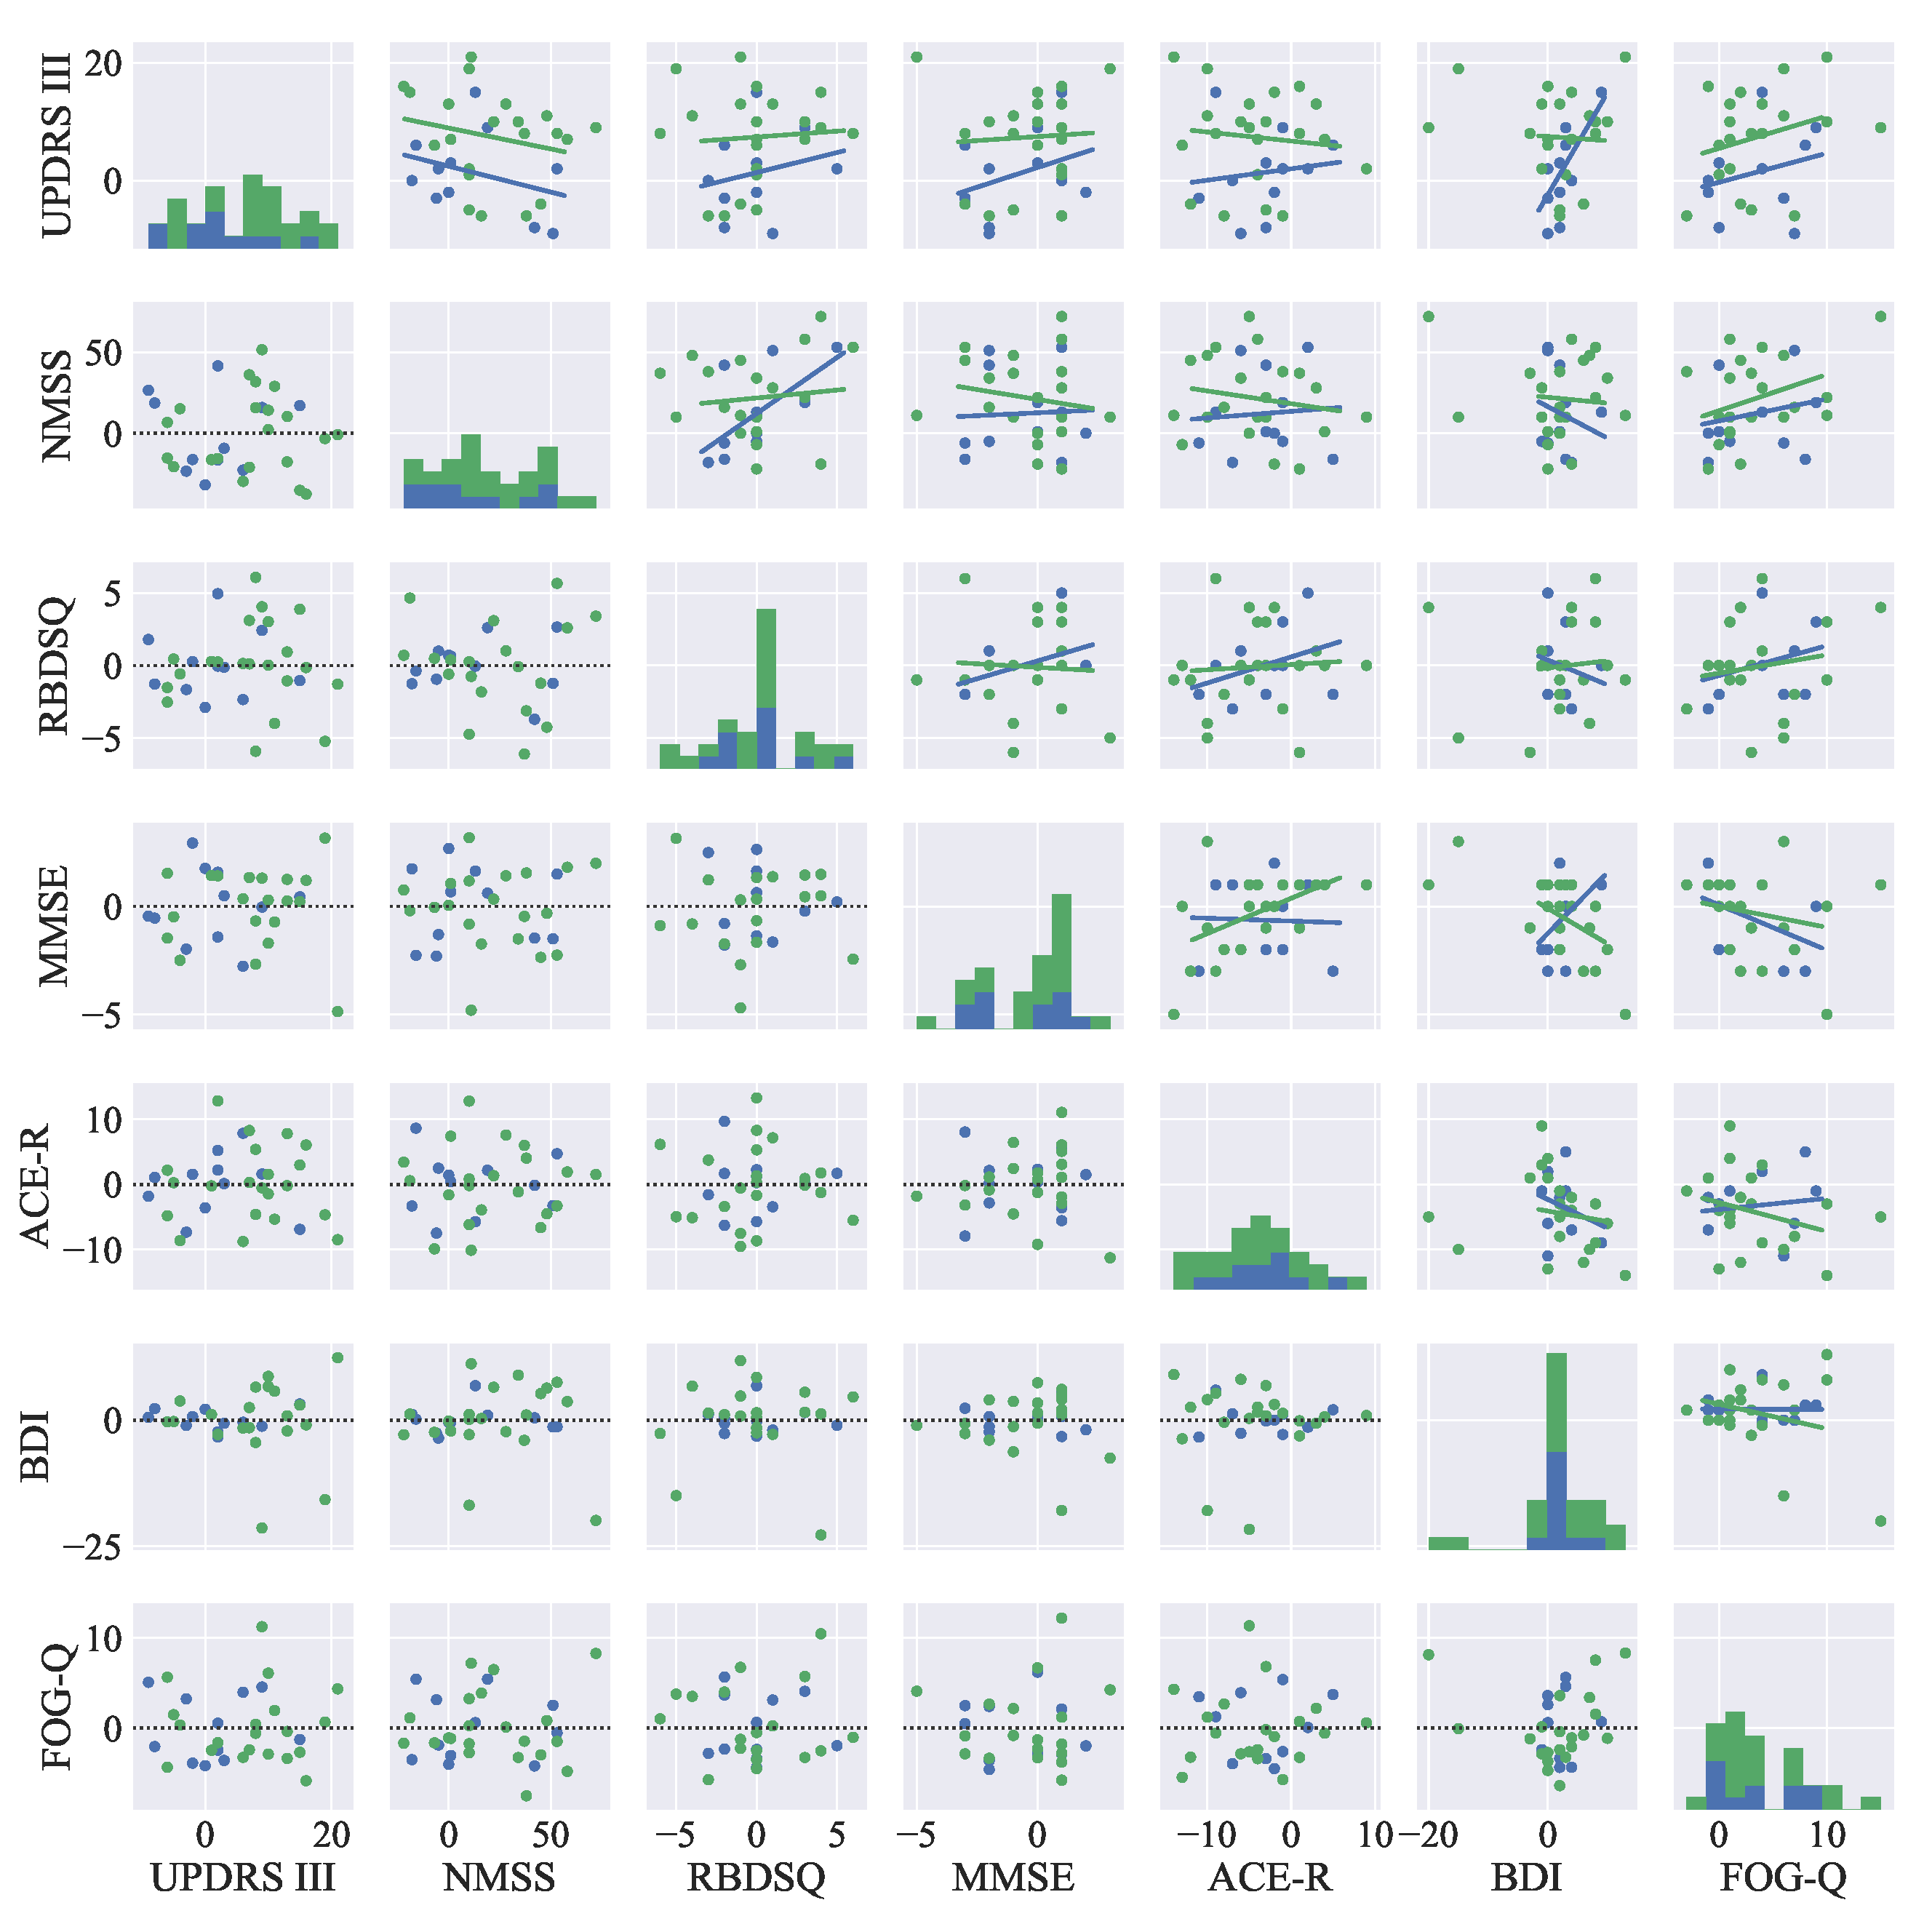
\includegraphics[width=0.99\textwidth]{pictures/ch6_clinical_statistics.eps}
	\caption[Descriptive statistical graphs of clinical data for PD patients.]{Descriptive statistical graphs of clinical characteristics of PD patients participated in this study (data for the $\delta$ session ($\mbox{session 2} - \mbox{session 1}$) only): on the main diagonal, histograms are visualized. Next, the upper triangular part of the graph-grid shows scatter plots with the fitted lines of the linear regression models. And finally, the lower triangular part of the graph-grid is used to display residuals for the models shown in the the upper grid. Colour notation: blue colour represents female speakers, and green colour represents male speakers. For the description of the rating scales, see Table~\ref{tab:ch6_clinical_data}}
	\label{fig:ch6_clinical_statistics}
\end{figure}

\newpage
With respect to the assessment of gait freezing, every patient was examined by a~trained movement disorders specialist who rated the gait-related difficulties according to a~specialized six-item Likert-scale ($5$-point scale where a~score of $0$ indicates absence of the symptom, while a~score of $4$~indicates the most severe stage; therefore the total score ranges from $0$--$24$): Freezing of gait questionnaire~\cite{Giladi2000}. Full template can be seen in Appendix~\ref{tab:FOGQ_template}. The scale can be theoretically divided into two parts: 1st part (question\,$1$--question\,$2$) assesses walking and gait-related difficulties affecting patient's daily activities and independence; 2nd part (question\,$3$--question\,$6$) assesses gait freezing specifically. There is also a~total score (T) computed as a~sum of the two sub-scores ($\mbox{T}_1$ for Q1--Q2, and $\mbox{T}_2$ for Q3--Q6) summarizing the two parts ($\mbox{T} = \mbox{T}_1 + \mbox{T}_2$, where $\mbox{T}_1 = \mbox{Q1} + \mbox{Q2}$, and $\mbox{T}_2 = \mbox{Q3} + \mbox{Q4} + \mbox{Q5} + \mbox{Q6}$). This study was focused on gait freezing exclusively, therefore only the second part of the questionnaire and its total score are considered.

Furthermore, to provide more insight into the evolution of gait-related deficits (specifically Q6--Q6 score and the total score (sum of Q1--Q6)) between the two examinations (session $1$, and session $2$), box plots are presented as well. These graphs can be seen in Figure~\ref{fig:ch6_boxplots}. For the purpose of this visualization, all samples from both sessions were used (as opposed to the descriptive statistical graphs shown in Figure~\ref{fig:ch6_clinical_statistics} in which only a~subset of speakers with no missing data was selected). The reason behind this is to show a~distribution of the data based on as much observations as possible to better approximate the reality.

\begin{figure}[htb!]
	\centering
	\scriptsize
	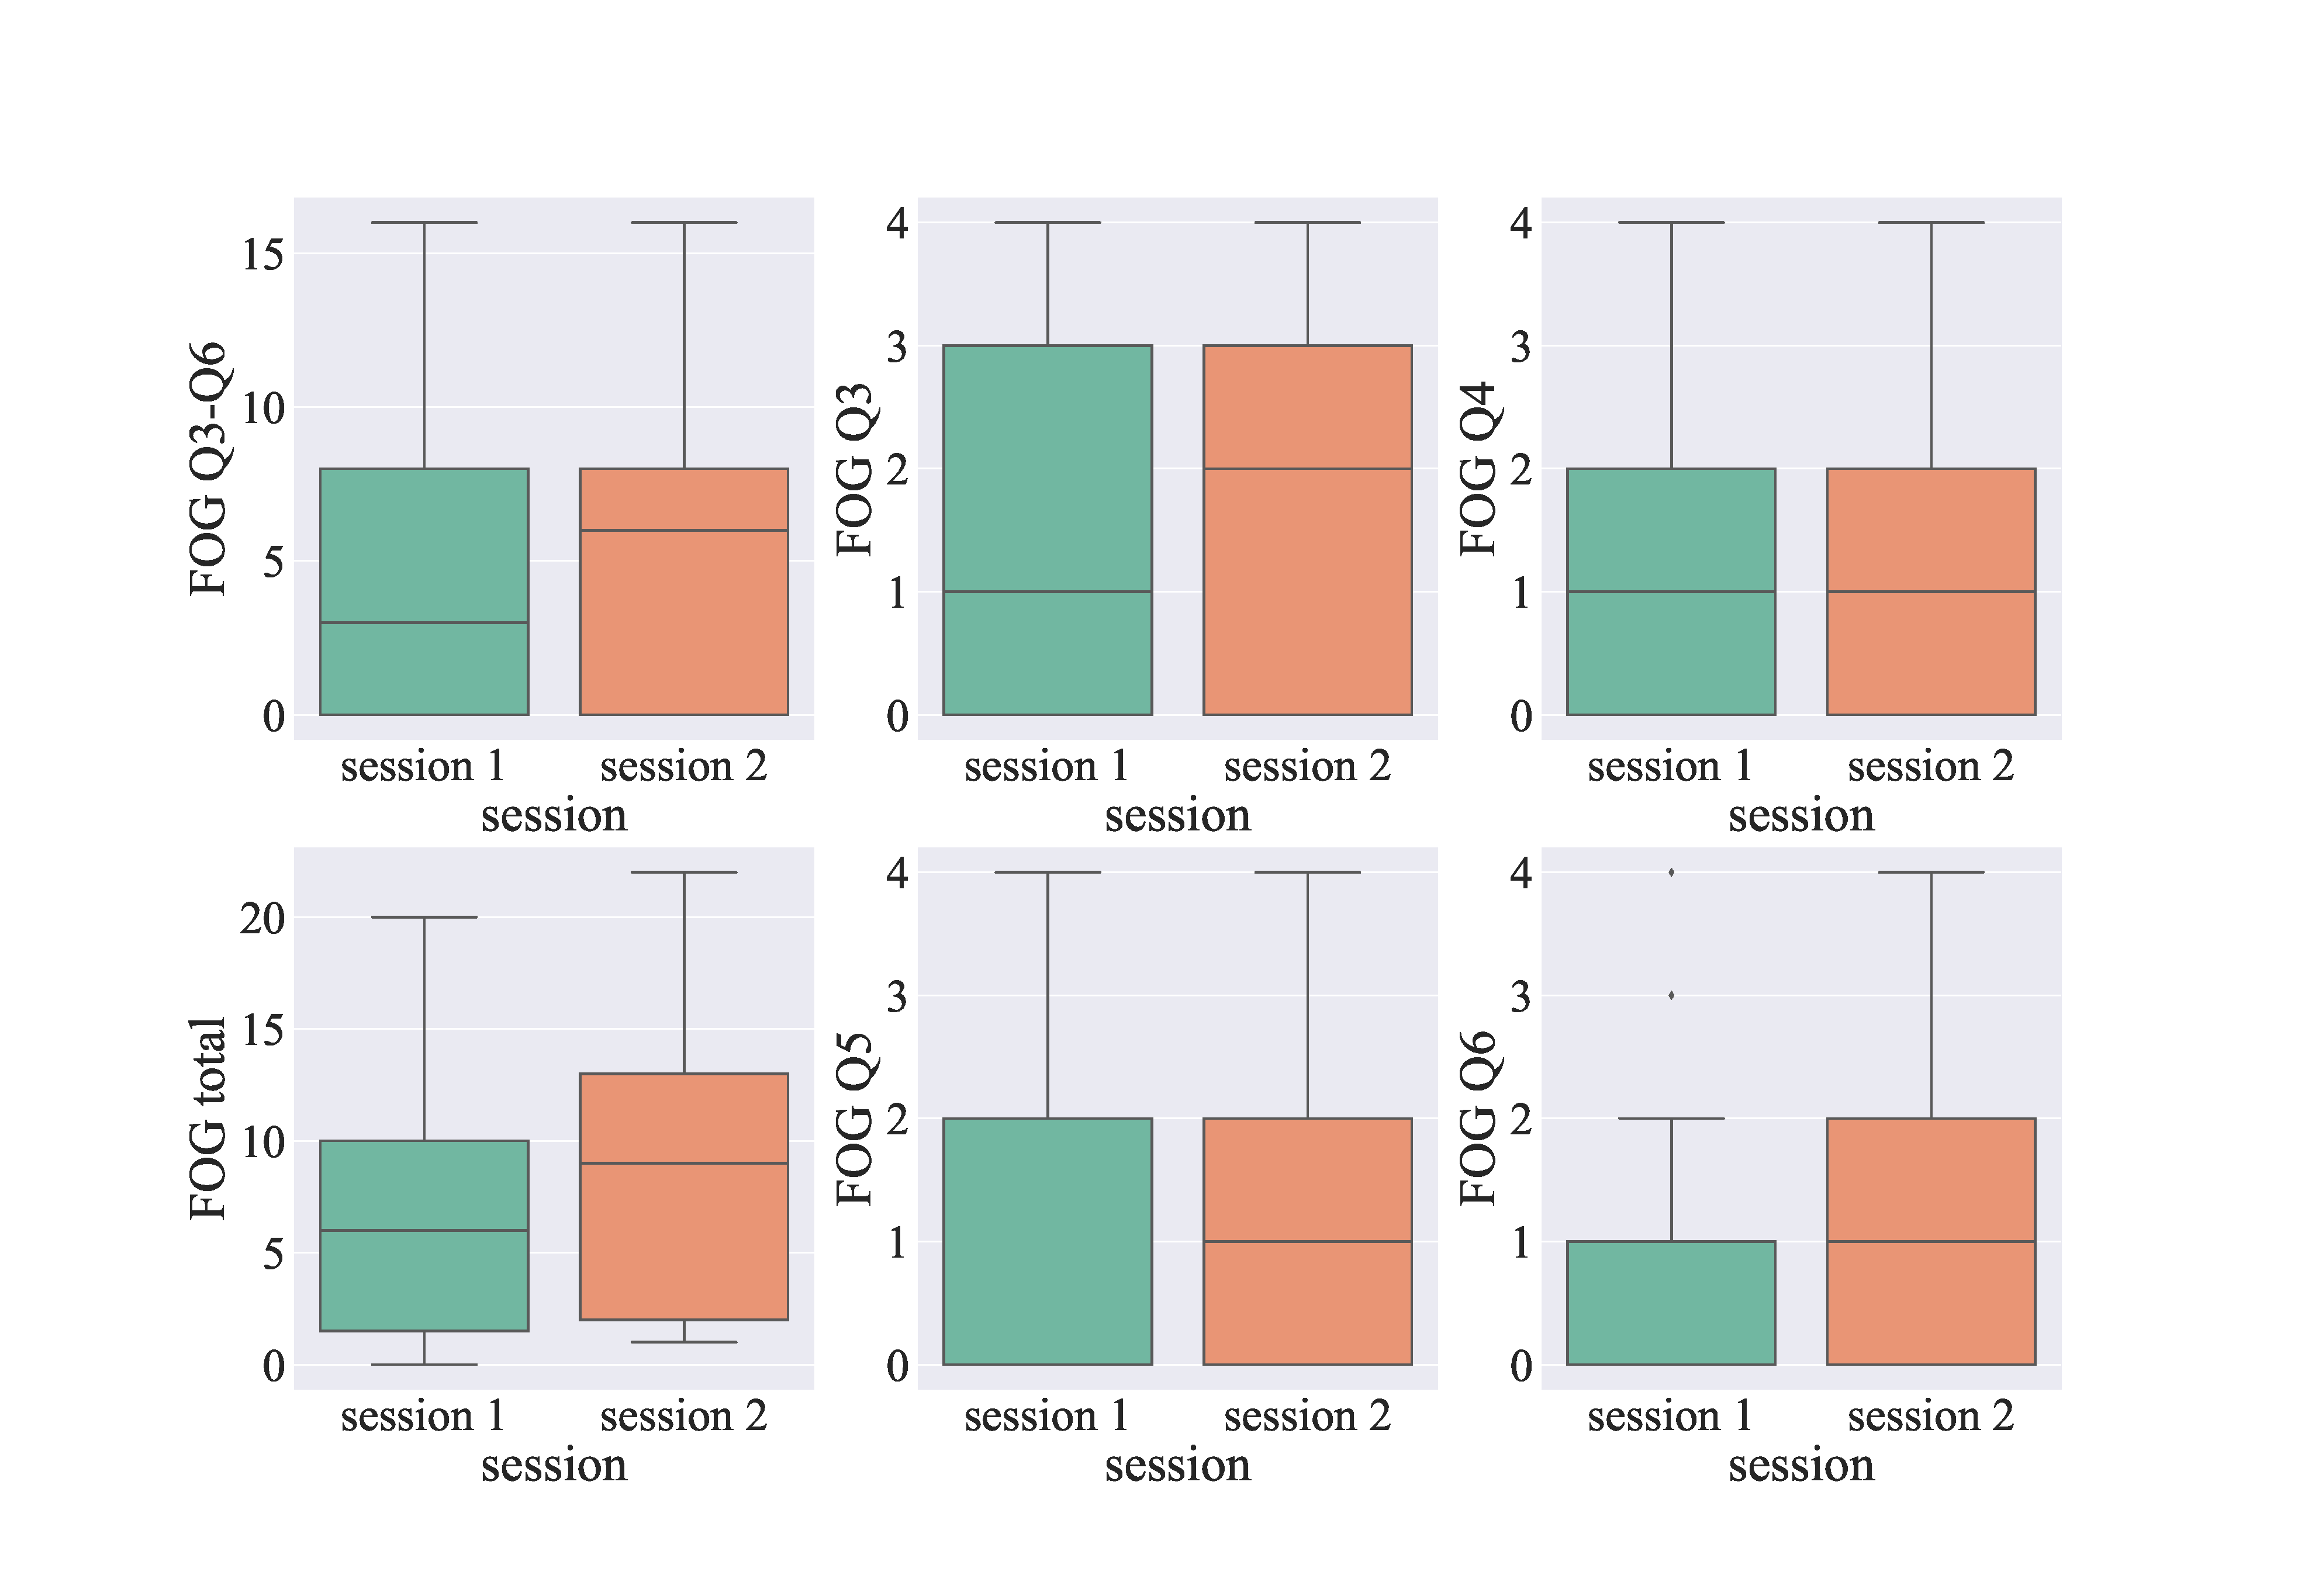
\includegraphics[width=0.99\textwidth]{pictures/ch6_box_plots_clin_fog.eps}
	\caption[Box plots for clinical data (gait assessment).]{Box plots visualizing the evolution of gait-specific deficits assessed by FOG-Q, specifically Q3--Q6 score and the total score (sum of Q1--Q6). Colour notation: green colour represents data for session $1$ (baseline examination), and blue colour represents data for session $2$ (follow-up examination).}
	\label{fig:ch6_boxplots}
\end{figure}

Regarding the speech task used to quantify HD, a~complex set of tasks was used to robustly quantify voice/speech disorders occurring with this disease. The speech acquisition protocol was actually derived from the standardized 3F Dysarthria Profile~\cite{Kostalova2013} and included fourteen speech tasks, specifically: monologue, expiration with closed/open lips, sustained phonation (/a/, /i/), diadochokinesis, rhythmical units, basic intonation/stress templates, and reading with different/no emotions. More complete description of these speech tasks can be seen in Table~\ref{tab:ch6_speech_tasks}. And finally, the actual acquisition of the acoustic signals was performed exactly in the same way as in the other studies summarized in this thesis. For more information, see chapter~\ref{ch4}.

\begin{table*}[htb!]
	\centering
	\begin{threeparttable}
		\caption{List of the examination speech tasks.}
		\label{tab:ch6_speech_tasks}
		\footnotesize
		\centering
		\begin{tabularx}{1.00\textwidth}{l l X}

			\hline\hline\noalign{\smallskip}
			\rowcolor{gray_table}
			label & vocal task & description \\
			\noalign{\smallskip}\hline\noalign{\smallskip}

			T1 & 
			Monologue & 
			Free speech without the interruption of a~clinician. The participants were instructed to speak about their daily living, hobbies, family, an so on. \\
			
			T2 & 
			Expiration with closed lips & 
			Sustained phonation of the consonant /m/ with closed lips as constantly and for as long as possible. It should be performed in one breath if possible. \\
			
			T3 & 
			Expiration with open lips & 
			Sustained phonation of the vowel /i/ with open lips as constantly and for as long as possible. It should be performed in one breath if possible. \\
			
			T4 & 
			Sustained phonation & 
			Sustained phonation of the vowel /a/ at a~comfortable pitch and loudness. Performed in one breath and without any limitations in length. \\
			
			T5 & 
			Diadochokinetic task & 
			Rapid and steady /pa/-/ta/-/ka/ syllable repetition as constantly and for as long as possible. It should be performed in one breath if possible. \\
			
			T6 & 
			Rhythmical units & 
			Reading a~text containing 4 rhymes of 16 words rhythmically (i.\,e. poem recitation, for more information about the task, see description in Chapter~\ref{ch4}). \\
			
			T7 & 
			Basic intonation template & 
			Short sentence reading containing 3 words. The sentence should be pronounced interrogatively (i.\,e. stress-modified reading, similar to Chapter~\ref{ch4}). \\
			
			T8 & 
			Basic intonation template & 
			Short sentence reading containing 3 words. The sentence should be pronounced imperatively (i.\,e. stress-modified reading, similar to Chapter~\ref{ch4}). \\
			
			T9 & 
			Basic intonation template & 
			Short sentence reading containing 3 words. The sentence should be pronounced declaratively (i.\,e. stress-modified reading, similar to Chapter~\ref{ch4}). \\
			
			T10 & 
			Reading paragraph & 
			Reading phonetically unbalanced text of 135 words. \\
			
			T11 & 
			Reading with different emotions & 
			Reading a~sentence of 8 words neutrally. \\
			
			T12 & 
			Reading with different emotions & 
			Reading a~sentence of 6 words angrily. \\
			
			T13 & 
			Reading with different emotions & 
			Reading a~sentence of 9 words in a~bored manner. \\
			
			T14 & 
			Reading with different emotions & 
			Reading a~sentence of 5 words excitedly. \\

			\noalign{\smallskip}\hline\hline
		\end{tabularx}
	\end{threeparttable}
\end{table*}

\subsection{Feature extraction}
\label{ch6_3_2}

To quantify voice/speech disorders in the PD patients, a~set of acoustic features based on a~recommendation given in recent review on acoustic analysis of voice/speech signals in patients suffering from HD~\cite{Brabenec2017} was computed. It specifically covers the area of phonation (Appendix~\ref{tab:phonatory_features}), articulation (Appendix~\ref{tab:articulation_features}), and prosody (Appendix~\ref{tab:prosodic_features}). To provide better insight into ability of these features to describe HD, a~short description per HD area is presented.

In terms of phonation, the acoustic features describing airflow insufficiency (MPT) during expiration with closed (T2) or opened (T3) lips, irregular pitch fluctuations (relF0SD) during phonation of the vowel /a/ (T4), microperturbations in frequency (jitter) and amplitude (shimmer) during phonation of the vowel /a/ (T4), tremor of jaw (F1SD, F2SD) during phonation of the vowel /a/ (T4), increased acoustic noise (mean HNR) during phonation of the vowel /a/ (T4), and aperiodicity of voice (DUV) during phonation of the vowel /a/ (T4) were computed.

With respect to articulation, the acoustic features describing rigidity of tongue and jaw (F1IR, F2IR, F1SD, F2SD) during monologue (T1), rhythmical reading (T6), basic intonation templates (T7--9), paragraph reading (T10), and reading with different emotions (T11--14), slow alternating motion rate (DDK rate) during diadochokinetic task (T5), and irregular alternating motion rate (DDK reg) during diadochokinetic task (T5) were computed.

Finally, regarding the acoustic features describing monopitch (relF0SD) and monoloudness (relSEOSD) during monologue (T1), rhythmical reading (T6), basic intonation templates (T7--9), paragraph reading (T10), and reading with different emotions (T11--14), inappropriate silences (SPIR) during paragraph reading (T10), unnatural speech rate (TSR, NSR) during basic intonation templates (T7--9), paragraph reading (T10), and reading with different emotions (T11--14) were computed.

\subsection{Analytical setup}
\label{ch6_3_3}

To assess the strength of a~relationship between the patients' clinical data and the selected items of FOG-Q in both sessions (session $1$, session $2$), Pearson's correlation with the significance level $0.05$ was used. With this approach, it was possible to identify those clinical measures (PD duration, UPDRS~III, LED (mg/day), NMSS, RBDSQ, MMSE, ACE-R, BDI) that are significantly correlated with the specific symptoms of gait freezing in PD, which is a~very valuable information because it shows which clinical aspects of PD tend to be associated with FOG in the baseline and in the follow-up (after $2$ years). Using the $\delta$ session ($\mbox{session 2} - \mbox{session 1}$), it is even possible to see if the evolution of other clinical aspects of PD is related with the evolution of the associated gait problems.

Next, to assess the strength of a~relationship between voice/speech disorders in HD and freezing of gait in patients with PD, Pearson's (linear relationship) and Spearman's (monotonic relationship) partial correlation coefficients\footnote{Partial correlation measures the unbiased degree of association between two variables while controlling for the effect of other confounding factors (variables).} between the acoustic features and the values of FOG-Q were computed. The significance level of correlation in this case was set to $0.05$ as well. During the computation of partial correlations, the factors such as patients' age and gender \cite{Skodda2011d, Vergara2017}, dopaminergic medication~\cite{Lee2010} and a~variety of associated motor and non-motor symptoms assessed by UPDRS~III~\cite{Fahn1987}, BDI \cite{Beck2000, Beck1961}, and ACE-R~\cite{Larner2007} were controlled for. As in the previous case, the aim was to identify those acoustic features that are significantly correlated with the specific symptoms of gait freezing in PD.

Finally, to evaluate the power of the acoustic features (in session $1$; baseline) in predicting the change of the severity of gait freezing in PD ($\Delta\,\mbox{FOG-Q}$), multivariate regression analysis was performed. For this purpose, we employed classification and regression trees (CART) in the supervised machine learning setup using stratified $10$-fold cross-validation with $100$ repetitions)~\cite{Breiman1984}. As previously, see Chapter~\ref{ch4} and Chapter~\ref{ch5}, feature selection process was applied to obtain the feature sets with the maximum clinical interpretability and also the power to predict FOG-related deficits in patients with PD. For this purpose, a~modified version of sequential floating forward selection~\cite{Pohjalainen2014} algorithm was used. To evaluate the prediction performance of the trained models, mean absolute error (MAE), root mean squared error (RMSE), and estimation error rate (EER) were computed. For more information about these metrics, see Chapter~\ref{ch5}.

\section{Results}
\label{ch6_4}

Regarding the classical correlation analysis, the values of Pearson's correlation coefficients computed between clinical data (e.\,g. scores of the clinical rating scales assessing motor and non-motor symptoms of PD) and selected items of FOG-Q (i.\,e. Q3--Q6, and the total score) can be found in Table~\ref{tab:ch6_classical_correlations}. This type of correlation was computed for all three sessions: session $1$ (baseline examination), session $2$ (follow-up examination), and $\delta$ session (description of the change in the particular item of the rating scale) The results are discussed bellow.

\begin{table*}[htb!]
	\centering
	\begin{threeparttable}
		\caption{Correlations among patients' FOG-Q items and clinical description.}
		\label{tab:ch6_classical_correlations}
		\footnotesize
		\centering
		\begin{tabular}{l r c r c r c r c r c}

			\hline\hline\noalign{\smallskip}
			\rowcolor{gray_table}
			FOG-Q & $\rho$\,(Q3) & $p$ & $\rho$\,(Q4) & $p$ & $\rho$\,(Q5) & $p$ & $\rho$\,(Q6) & $p$ & $\rho$\,(total) & $p$ \\
			\noalign{\smallskip}
			\multicolumn{11}{c}{Session 1} \\
			\noalign{\smallskip}\hline\noalign{\smallskip}

			PD dur. (years)  &  0.47 & ** &  0.35 & ** &  0.35 & ** &  0.39 & ** &  0.44 & ** \\
			UPDRS III        &  0.24 & *  &  0.24 & *  &  0.24 &    &  0.23 & *  &  0.25 & *  \\
			LED (mg/day)     &  0.36 & ** &  0.33 & ** &  0.37 & ** &  0.24 & *  &  0.37 & ** \\
			NMSS             &  0.45 & ** &  0.43 & ** &  0.39 & ** &  0.52 & ** &  0.49 & ** \\
			RBDSQ            &  0.25 & *  &  0.28 & *  &  0.14 &    &  0.28 & *  &  0.27 & *  \\
			MMSE             & -0.01 &    & -0.07 &    &  0.06 &    & -0.06 &    & -0.02 &    \\
			ACE-R            & -0.06 &    & -0.15 &    &  0.04 &    & -0.13 &    & -0.08 &    \\
			BDI              &  0.05 &    &  0.06 &    &  0.09 &    &  0.13 &    &  0.09 &    \\

			\noalign{\smallskip}\hline\noalign{\smallskip}
			\multicolumn{11}{c}{Session 2} \\
			\noalign{\smallskip}\hline\noalign{\smallskip}

			PD dur. (years)  &  0.41 & ** &  0.41 & ** &  0.38 & ** &  0.42 & ** &  0.44 & ** \\
			UPDRS III        &  0.36 & *  &  0.45 & ** &  0.35 & *  &  0.39 & *  &  0.42 & ** \\
			LED (mg/day)     &  0.28 &    &  0.03 &    &  0.17 &    &  0.15 &    &  0.18 &    \\
			NMSS             &  0.39 & *  &  0.30 &    &  0.26 &    &  0.36 & *  &  0.36 & *  \\
			RBDSQ            &  0.34 & *  &  0.28 &    &  0.38 & *  &  0.41 & ** &  0.38 & *  \\
			MMSE             & -0.26 &    & -0.14 &    & -0.14 &    & -0.07 &    & -0.17 &    \\
			ACE-R            & -0.25 &    & -0.18 &    & -0.18 &    & -0.13 &    & -0.20 &    \\
			BDI              &  0.36 & *  &  0.36 & *  &  0.38 & *  &  0.38 & *  &  0.40 & ** \\

			\noalign{\smallskip}\hline\noalign{\smallskip}
			\multicolumn{11}{c}{$\Delta$ (Session 2 $-$ Session 1)} \\
			\noalign{\smallskip}\hline\noalign{\smallskip}

			PD dur. (years)  & -0.22 &    &  0.06 &    &  0.18 &    &  0.25 &    &  0.04 &    \\
			UPDRS III        &  0.03 &    &  0.17 &    &  0.17 &    &  0.10 &    &  0.16 &    \\
			LED (mg/day)     & -0.28 &    & -0.33 &    & -0.35 &    & -0.18 &    & -0.40 & *  \\
			NMSS             &  0.20 &    &  0.04 &    &  0.20 &    &  0.42 & *  &  0.28 &    \\
			RBDSQ            &  0.09 &    &  0.24 &    &  0.06 &    &  0.24 &    &  0.21 &    \\
			MMSE             & -0.35 & *  & -0.26 &    & -0.29 &    & -0.12 &    & -0.36 & *  \\
			ACE-R            & -0.17 &    & -0.25 &    & -0.24 &    & -0.06 &    & -0.25 &    \\
			BDI              & -0.26 &    & -0.10 &    & -0.06 &    &  0.02 &    & -0.16 &    \\

			\noalign{\smallskip}\hline\hline
		\end{tabular}

		\begin{tablenotes}
			\scriptsize
			\item[1] Table notation: $\rho$\,--\,Spearman's correlation coefficient; $p$\,--\,significance level of correlation (* means $p<0.05$; ** means $p<0.01$); UPDRS~III\,--\,Unified Parkinson's disease rating scale, part~III: evaluation of motor function~\cite{Fahn1987}; LED\,--\,L-dopa equivalent daily dose~\cite{Lee2010}; NMSS\,--\,Non-motor symptoms scale~\cite{Chaudhuri2007}; RBDSQ\,--\,The REM sleep behavior disorder screening questionnaire~\cite{Stiasny2007}; MMSE\,--\,Mini-mental state examination~\cite{Folstein1975}; ACE-R\,--\,Addenbrooke's cognitive examination-revised~\cite{Larner2007}; BDI\,--\,Beck depression inventory \cite{Beck2000, Beck1961}; FOG-Q\,--\,Freezing of gait questionnaire~\cite{Giladi2000} (Q1--Q6, and T\,--\,total score), for more details, see Section~\ref{tab:ch6_clinical_data}.
		\end{tablenotes}
	\end{threeparttable}
\end{table*}

In both sessions, significant correlations of all FOG-Q items with duration of PD and UPDRS~III (except Q5 in session $1$) were identified. Next, LED was found significantly correlated with all FOG-Q items in session $1$, but not in the session $2$. Next, NMSS and all items of FOG-Q were found significantly correlated in session $1$, however in the session $2$ only few significant correlations were found. Regarding RBDSQ, no specific pattern can be observed. FOG-Q items correlated variably with RBDSQ, however, significant correlation for FOG-Q (total score) was found in both sessions. The scales assessing cognitive functions (MMSE, ACE-R) were not find significantly correlated with the items of FOG-Q. And finally, BDI score was not found significantly correlated with FOG-Q in session $1$. Nevertheless, significant correlations can be observed in session $2$. Regarding the correlations between $\Delta\,(\mbox{Q3--6, total score})$ and $\Delta$ of the clinical scores, significant correlations between the changes in FOG-Q items and changes in LED, NMSS and MMSE were identified. Next, the results for partial correlation analysis are summarized in Table~\ref{tab:ch6_partial_correlations}. The associated regression plots can be seen in Figure~\ref{fig:ch6_correlation_plots}.

\begin{table*}[htb!]
\centering
	\begin{threeparttable}
		\caption{Partial correlations among features and FOG-Q (session 1) items.}
		\label{tab:ch6_partial_correlations}
		\footnotesize
		\centering
		\begin{tabular}{l l l r c r c}
			
			\hline\hline\noalign{\smallskip}
			\rowcolor{gray_table}
			HD area & specific disorder & features & $\rho$\,(P) & $p$\,(P) & $\rho$\,(S) & $p$\,(S) \\
			\noalign{\smallskip}
			\multicolumn{7}{c}{FOG\,(Q3)} \\
			\noalign{\smallskip}\hline\noalign{\smallskip}

			prosody      & unnatural speech rate      & NSR\,(T8)   &  0.41 & ** &  0.34 & *  \\
			articulation & rigidity of tongue and jaw & F1IR\,(T10) & -0.40 & ** & -0.44 & ** \\
			articulation & rigidity of tongue and jaw & F1IR\,(T9)  & -0.34 & *  & -0.38 & ** \\
			articulation & rigidity of tongue and jaw & F1IR\,(T13) & -0.32 & *  & -0.39 & ** \\
			articulation & rigidity of tongue and jaw & F1IR\,(T14) & -0.30 & *  & -0.30 & *  \\
			articulation & rigidity of tongue and jaw & F1IR\,(T7)  & -0.30 & *  & -0.35 & *  \\
			
			\noalign{\smallskip}\hline\noalign{\smallskip}
			\multicolumn{7}{c}{FOG\,(Q4)} \\
			\noalign{\smallskip}\hline\noalign{\smallskip}

			articulation & rigidity of tongue and jaw & F1IR\,(T10) & -0.40 & ** & -0.43 & ** \\
			articulation & rigidity of tongue and jaw & F1IR\,(T9)  & -0.35 & *  & -0.40 & ** \\
			
			\noalign{\smallskip}\hline\noalign{\smallskip}
			\multicolumn{7}{c}{FOG\,(Q5)} \\
			\noalign{\smallskip}\hline\noalign{\smallskip}

			articulation & rigidity of tongue and jaw & F1IR\,(T14) & -0.47 & ** & -0.49 & ** \\
			prosody      & unnatural speech rate      & NSR\,(T8)   &  0.36 & *  &  0.42 & ** \\
			articulation & rigidity of tongue and jaw & F1IR\,(T10) & -0.36 & *  & -0.40 & ** \\
			articulation & rigidity of tongue and jaw & F1IR\,(T13) & -0.29 & *  & -0.36 & *  \\
			
			\noalign{\smallskip}\hline\noalign{\smallskip}
			\multicolumn{7}{c}{FOG\,(Q6)} \\
			\noalign{\smallskip}\hline\noalign{\smallskip}

			prosody      & unnatural speech rate      & TSR\,(T11)  &  0.33 & *  &  0.33 & *  \\
			prosody      & unnatural speech rate      & NSR\,(T8)   &  0.33 & *  &  0.33 & *  \\
			prosody      & unnatural speech rate      & NSR\,(T11)  &  0.32 & *  &  0.32 & *  \\

			\noalign{\smallskip}\hline\noalign{\smallskip}
			\multicolumn{7}{c}{FOG\,(total score)} \\
			\noalign{\smallskip}\hline\noalign{\smallskip}

			articulation & rigidity of tongue and jaw & F1IR\,(T10) & -0.40 & ** & -0.45 & ** \\
			articulation & rigidity of tongue and jaw & F1IR\,(T14) & -0.38 & ** & -0.38 & ** \\
			articulation & unnatural speech rate      & NSR\,(T8)   &  0.36 & *  &  0.38 & ** \\
			
			\noalign{\smallskip}\hline\hline
		\end{tabular}
	
		\begin{tablenotes}
			\scriptsize
			\item[1] Table notation: $\rho$\,(P)\,--\,Pearson's correlation coefficient; $p$\,(S)\,--\,significance level of correlation according to $\rho$\,(P); $\rho$\,(S)\,--\,Spearman's correlation coefficient; $p$\,(S)\,--\,significance level of correlation according to $\rho$\,(S) (* means $p<0.05$; ** means $p<0.01$); FOG-Q\,--\,Freezing of gait questionnaire~\cite{Giladi2000}.
		\end{tablenotes}
	\end{threeparttable}
\end{table*}

\begin{figure}[htb!]
	\centering
	\scriptsize
	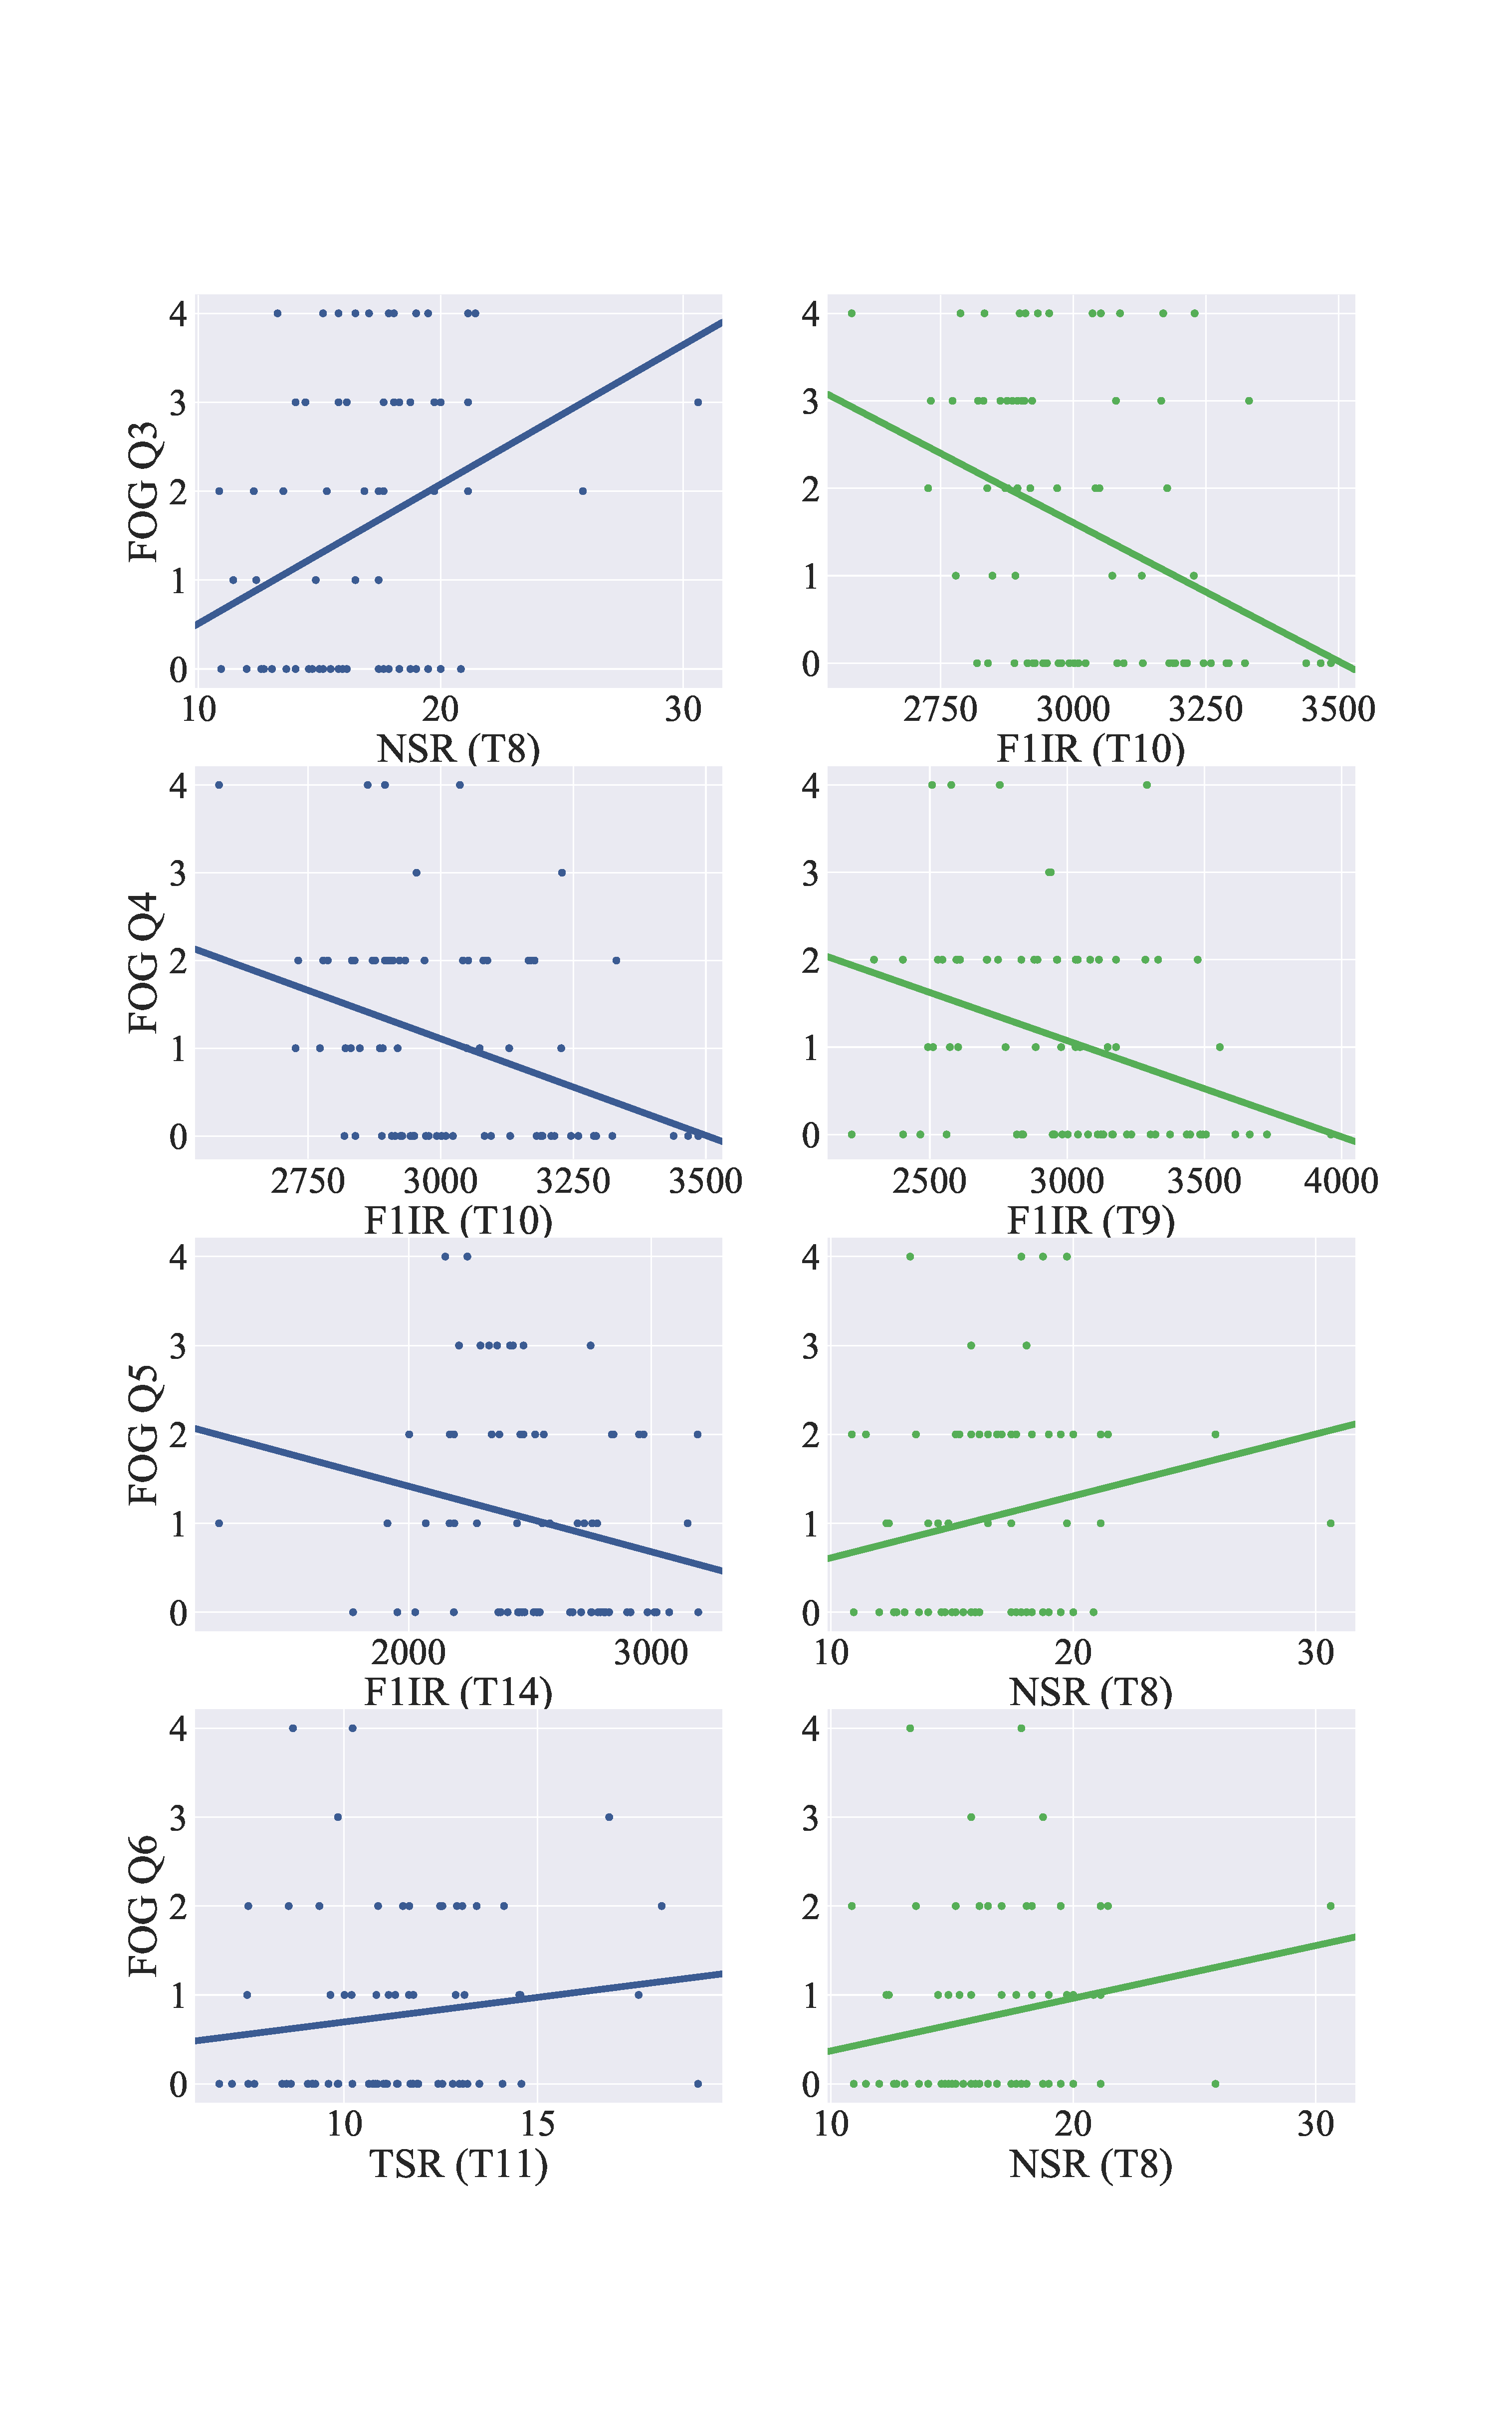
\includegraphics[width=0.80\textwidth]{pictures/ch6_correlation_plots.eps}
	\caption[Regression plots for FOG-Q (Q3--Q6).]{Regression plots (scatter plots with the fitted line of the robust linear regression estimator) of the most correlated acoustic features (partial correlation) for Q3--Q6, see Table~\ref{tab:ch6_partial_correlations}. Colour notation: blue colour represents the most correlated feature; and green colour represents the second most correlated feature. For speech task notation, see Table~\ref{tab:ch6_speech_tasks}.}
	\label{fig:ch6_correlation_plots}
\end{figure}

With respect to the partial correlation analysis, the correlations among acoustic features quantifying impaired phonation, articulation and prosody, and selected items of FOG-Q (Q3--Q6, and the total score) were computed. It is important to point out that the partial correlation analysis was performed for session $1$ only to focus on the investigation of the relationship between FOG and HD in the baseline. For a~better overview, only the acoustic features with significant correlation in both Pearson's, and Spearman's correlations were selected. Regarding Q3 (assessment of occurrence of freezing), this item was found correlated mostly with the interpercentile range of the first formant, and with net speech rate (extracted from reading of a~short sentence). The strongest correlation can be seen in the case of NSR extracted from the short imperative sentence reading ($\rho\,(\mbox{P})=-0.40$, $p<0.01$, and $\rho\,(\mbox{S})=-0.44$, $p<0.01$). In the case of Q4 (assessment of the duration of the longest freezing episode), $2$ significant negative correlations were identified for the interpercentile range of the first formant (extracted from paragraph reading, and short declarative sentence reading). The strongest correlation can be seen in the case of paragraph reading ($\rho\,(\mbox{P})=-0.40$, $p<0.01$, and $\rho\,(\mbox{S})=-0.43$, $p<0.01$). With respect to Q5 (assessment of the duration of the typical start hesitation), the interpercentile range of the first formant (extracted from paragraph reading, reading of $9$ words in a~bored manner, reading of $5$ words excitedly), and with the net speech rate (extracted from short imperative sentence reading) were found significantly correlated with this particular item of the questionnaire. The strongest correlation can be seen in the case of F1IR extracted from the reading of $5$ words in an~excited manner ($\rho\,(\mbox{P})=-0.47$, $p<0.01$, and $\rho\,(\mbox{S})=-0.49$, $p<0.01$). In the case of Q6 (assessment of the duration of the typical turning hesitation), significant correlations were found for total speech rate (extracted from reading of a~sentence of $8$ words in a~neutral manner) and net speech rate (extracted from short imperative sentence reading and reading of a~sentence of $8$ words in a~neutral manner). The strongest correlation can be seen in the case of TSR extracted from the reading of a~sentence of $8$ words in a~neutral manner ($\rho\,(\mbox{P})=0.33$, $p<0.05$, and $\rho\,(\mbox{S})=0.33$, $p<0.05$). And finally, with respect to the total score (Q3--Q6), interpercentile range of the first formant (extracted from paragraph reading and reading of $5$ words excitedly), and net speech rate (extracted from short imperative sentence reading) were found significantly correlated with this item. The strongest correlation can be seen in the case of F1IR extracted from the paragraph reading ($\rho\,(\mbox{P})=-0.40$, $p<0.05$, and $\rho\,(\mbox{S})=-0.45$, $p<0.05$). Next, the results of the multivariate regression analysis can be seen in Table~\ref{tab:ch6_regression_analysis}. Moreover, the models for FOG-G (Q5), and FOG (Q6) are visualized (visualization of the approximation of decision making performed by the regression tree) using the three graphs, see Figure~\ref{fig:ch6_regression_tree_fogq5}, and Figure~\ref{fig:ch6_regression_tree_fogq6}, respectively.

\begin{table*}[htb!]
\centering
	\begin{threeparttable}
		\caption{FOG deficits prediction using classification and regression trees.}
		\label{tab:ch6_regression_analysis}
		\footnotesize
		\centering
		\begin{tabular}{l r r r c l}
			
			\hline\hline\noalign{\smallskip}
			\rowcolor{gray_table}
			FOG-Q & MAE & RMSE & EER & No. & selected features \\
			\noalign{\smallskip}
			\multicolumn{6}{c}{Articulation} \\
			\noalign{\smallskip}\hline\noalign{\smallskip}

			Q3 & 0.86~$\pm$~0.26 & 1.03~$\pm$~0.28 & 20.96~$\pm$~6.38 & 1 & F1SD$^{11}$ \\
			Q4 & 0.76~$\pm$~0.28 & 0.89~$\pm$~0.31 & 20.78~$\pm$~7.73 & 2 & F1IR$^{6}$,\,F2SD$^{14}$ \\
			Q5 & 0.49~$\pm$~0.22 & 0.64~$\pm$~0.34 & 10.52~$\pm$~4.67 & 4 & F2SD$^{7}$,\,F1IR$^{11}$,\,F1SD$^{12}$,\,DDKr$^{5}$ \\
			Q6 & 0.60~$\pm$~0.28 & 0.77~$\pm$~0.43 & 13.85~$\pm$~6.41 & 1 & F1SD$^{6}$ \\
			T  & 2.15~$\pm$~0.63 & 2.53~$\pm$~0.73 & 21.89~$\pm$~6.44 & 1 & F1SD$^{9}$ \\

			\noalign{\smallskip}\hline\noalign{\smallskip}
			\multicolumn{6}{c}{Phonation} \\
			\noalign{\smallskip}\hline\noalign{\smallskip}

			Q3 & 1.11~$\pm$~0.30 & 1.29~$\pm$~0.33 & 27.11~$\pm$~7.33 & 1 & jitter$^{4}$ \\
			Q4 & 0.94~$\pm$~0.28 & 1.14~$\pm$~0.31 & 25.84~$\pm$~7.57 & 2 & shimmer$^{4}$,\,jitter$^{4}$ \\
			Q5 & 0.62~$\pm$~0.24 & 0.81~$\pm$~0.33 & 13.42~$\pm$~5.18 & 1 & MPT$^{3}$ \\
			Q6 & 0.60~$\pm$~0.24 & 0.79~$\pm$~0.34 & 13.95~$\pm$~5.57 & 1 & MPT$^{2}$ \\
			T  & 2.32~$\pm$~0.75 & 2.91~$\pm$~0.90 & 23.64~$\pm$~7.63 & 1 & relF0SD$^{4}$ \\

			\noalign{\smallskip}\hline\noalign{\smallskip}
			\multicolumn{6}{c}{Prosody} \\
			\noalign{\smallskip}\hline\noalign{\smallskip}

			Q3 & 0.85~$\pm$~0.33 & 1.04~$\pm$~0.39 & 20.90~$\pm$~8.01 & 3 & TSR$^{11}$,\,TSR$^{10}$,\,relF0SD$^{11}$ \\
			Q4 & 0.80~$\pm$~0.24 & 0.96~$\pm$~0.27 & 21.88~$\pm$~6.69 & 1 & TSR$^{7}$ \\
			Q5 & 0.56~$\pm$~0.22 & 0.71~$\pm$~0.31 & 12.09~$\pm$~4.77 & 3 & relSEOSD$^{9}$,\,SPIR$^{10}$,\,relF0SD$^{1}$ \\
			Q6 & 0.55~$\pm$~0.20 & 0.71~$\pm$~0.26 & 12.75~$\pm$~4.54 & 2 & TSR$^{7}$,\,NSR$^{14}$ \\
			T  & 2.07~$\pm$~0.71 & 2.59~$\pm$~0.88 & 21.10~$\pm$~7.20 & 4 & TSR$^{11}$,\,TSR$^{10}$,\,TSR$^{9}$,\,NSR$^{8}$ \\

			\noalign{\smallskip}\hline\noalign{\smallskip}
			\multicolumn{6}{c}{Combination} \\
			\noalign{\smallskip}\hline\noalign{\smallskip}

			Q3 & 0.83~$\pm$~0.27 & 1.01~$\pm$~0.31 & 20.40~$\pm$~6.73 & 3 & F1SD$^{11}$,\,relF0SD$^{6}$,\,F2IR$^{1}$ \\
			Q4 & 0.76~$\pm$~0.28 & 0.89~$\pm$~0.31 & 20.78~$\pm$~7.73 & 2 & F1IR$^{6}$,\,F2SD$^{14}$ \\
			Q5 & 0.51~$\pm$~0.21 & 0.66~$\pm$~0.32 & 11.03~$\pm$~4.59 & 3 & F2SD$^{7}$,\,relF0SD$^{4}$,\,F2SD$^{12}$ \\
			Q6 & 0.50~$\pm$~0.21 & 0.65~$\pm$~0.29 & 11.73~$\pm$~4.93 & 4 & TSR$^{7}$,\,HNRm$^{4}$,\,F2SD$^{7}$,\,TSR$^{11}$ \\
			T  & 2.00~$\pm$~0.69 & 2.48~$\pm$~0.82 & 20.35~$\pm$~7.08 & 3 & F1SD$^{9}$,\,TSR$^{11}$,\,F1IR$^{6}$ \\
	
			\noalign{\smallskip}\hline\hline
		\end{tabular}
	
		\begin{tablenotes}
		\scriptsize
			\item[1] Table notation: MAE\,--\,mean absolute error; RMSE\,--\,root mean squared error; EER\,--\,relative estimation error rate (mean absolute error divided by the range of actual values of clinical rating scale present in the dataset; expressed in $\%$); No.\,--\,number of selected features; feature$^{x}$\,--\,acoustic feature and the label of the speech task ($x$), see Section~\ref{tab:ch6_clinical_data}; FOG-Q\,--\,Freezing of gait questionnaire~\cite{Giladi2000} (Q3--Q6, and T\,--\,total score), for more details, see Section~\ref{tab:ch6_clinical_data} as well.
		\end{tablenotes}
	\end{threeparttable}
\end{table*}

\begin{figure}[htb!]
	\centering
	\scriptsize
	\includegraphics[width=0.99\textwidth]{pictures/ch6_tree_model_fogq5.pdf}
	\caption[Regression tree graph visualization for FOG-Q (Q5)]{Visualization of the regression tree built to estimate FOG-Q (Q5). The tree was trained using a~single run applied on all data (all speech tasks and all acoustic features) in the dataset for the features selected by the feature selection algorithm (hence the decision making of the tree is an approximation of the behavior responsible for the results summarized in Table~\ref{tab:ch6_regression_analysis}). In the case of this tree, three acoustic features are used: F2SD (T7), relF0SD (T4), and F2SD (T12).}
	\label{fig:ch6_regression_tree_fogq5}
\end{figure}

\begin{figure}[htb!]
	\centering
	\scriptsize
	\includegraphics[width=0.60\textwidth]{pictures/ch6_tree_model_fogq6.pdf}
	\caption[Regression tree graph visualization for FOG-Q (Q6)]{Visualization of the regression tree built to estimate FOG-Q (Q6). The tree was trained using a~single run applied on all data (all speech tasks and all acoustic features) in the dataset for the features selected by the feature selection algorithm (hence the decision making of the tree is an approximation of the behavior responsible for the results summarized in Table~\ref{tab:ch6_regression_analysis}). In the case of this tree, three acoustic features are used: TSR (T7), HNRm (T4), F2SD (T7), and TSR (T11).}
	\label{fig:ch6_regression_tree_fogq6}
\end{figure}

\newpage
Regarding the multivariate regression analysis, the results can be seen in Table~\ref{tab:ch6_regression_analysis}. The table contains the results related to the prediction of the change in FOG severity in a~two-year horizon. When considering the three HD dimensions separately, the following results were achieved. The change in Q3 was predicted with the estimation error of $20.96\,\%$ using $3$ prosodic features. Specifically, TSR (reading of a~sentence of $8$ words in a~neutral manner), TSR (paragraph reading), and relF0SD (reading of a~sentence of $8$ words in a~neutral manner). The change in Q4 was predicted with the estimation error of $20.78\,\%$ using $2$ articulatory features. Specifically, F1IR (rhythmical reading), and F2SD (reading of $5$ words in an~excited manner). The change in Q5 was predicted with the estimation error of $10.52\,\%$ using $4$ articulatory features. Specifically, F2SD (short interrogative sentence reading), F1IR (reading of a~sentence of $8$ words in a~neutral manner), F1SD (reading of a~sentence of $6$ words angrily), and DDKr (diadochokinetic task). The change in Q6 was predicted with the estimation error of $12.75\,\%$ using $2$ prosodic features. Specifically, TSR (short interrogative sentence reading), and NSR (reading of $5$ words in an~excited manner). The change in total score (Q3--Q6) was predicted with the estimation error of $21.10\,\%$ using $4$ prosodic features. Specifically, TSR (reading of a~sentence of $8$ words in a~neutral manner), TSR (paragraph reading), TSR (short declarative sentence reading), and NSR (short imperative sentence reading). And finally, when considering a~combination of the features, the prediction was improved in the case of Q3, Q6, and total score (the difference, i.\,e. improvement is shown [in percentage]): Q3 ($0.56$), Q6 ($1.02$), and total score ($0.75$). However, as can be seen, the improvements are not that significant, which shows a~strong relationship between separate HD areas and specific FOG deficits.

\section{Conclusion}
\label{ch6_5}

Regarding the correlation between the individual items of FOG-Q and other clinical signs of PD assessed by the previously mentioned clinical rating scales, the following conclusions can be drawn. The results proposed in this study (in both sessions) confirm the previous findings of Giladi et al.~\cite{Giladi2000} who reported a~significant correlation between UPDRS~III and FOG-Q. Next, a~strong association between duration of PD and severity of FOG, which is also in accordance with the previous findings \cite{Macht2007, Nilsson2009, Shine2013}, was identified. In addition to that, the results suggest that FOG-Q scores are no longer correlated with dopaminergic medication assessed by LED (mg/day) after the two-year follow-up, which is an interesting finding that points out to the fact that as the disease progresses, the FOG episodes loose their responsiveness to levodopa, or the effect of this medication is not as easily predictable anymore. This is in line with the literature that reports the unresponsiveness of FOG to levodopa as being more prevalent in the more advanced stages of PD, which is hypothesized to be a~consequence of higher importance and influence of other neurotransmitters and pathophysiological mechanisms besides those related to dopaminergic deficits \cite{Espay2012, Vercruysse2014, Xiao2017}. Next, FOG-Q items were found significantly correlated with non-motor symptoms of PD assessed by NMSS, which supports the findings of Zhang et al.~\cite{Zhang2016}, who pointed out the presence of the relationship between FOG and cardiovascular domain of the NMSS. With respect to RBDSQ, the total score of FOG-Q was found strongly related to the level of REM sleep behaviour disorder assessed by this particular rating scale. This is in line with the findings of several studies reporting that increased muscle activity during REM sleep is a~comorbid feature of patients with PD who exhibit FOG \cite{Videnovic2013, Walton2015, Zhang2016}. With respect to other non-motor symptoms of PD assessed by MMSE and ACE-R, none of the correlations were found significant. This is in contradiction with the previous studies that did demonstrate the presence of a~relationship between impaired cognitive functions and FOG \cite{Rektorova2016, Yao2017}. And finally, in the case of BDI, the significant correlations were found only in the follow-up session that is suggesting that the presence of more advanced depressive symptoms (although not severe enough to diagnose the major depressive episode) at the follow-up examination is linked with the progression of PD. This is also in accordance of the previous studies that showed depressive symptoms could be pertinent and significant predictors of FOG in PD \cite{Giladi2001b, Shine2013, Walton2015}.

Next, in the case of the partial correlation analysis between the acoustic features quantifying phonation, articulation and prosody in HD and selected items of FOG-Q, the following conclusions can be drawn. At first, it must be pointed out that no corrections for multiple comparisons was applied since after employing any of the most commonly-used methods for significance level adjustment such as Bonferroni correction~\cite{Weisstein2004} or false discovery rate (FDR)~\cite{Storey2011}, none of the correlations appeared to be significant (none of the p-values were bellow the chosen significance level of $0.05$). However, this is tightly linked to the number of cohorts in the dataset (to be discussed later). Therefore, the results of this analysis must be considered as exploratory and pilot in nature. So, with that in mind, it can be seen that most of the FOG-Q items, showed statistically significant correlation with the articulatory features, more specifically with the interpercentile range of first formant. Moreover, in some cases, standard deviation of the first formant was close to the significance level as well. To discuss this observation in more details, formants are resonances of the oro-naso-pharyngeal tract that are changed mainly by a~position of tongue and jaw \cite{Gomez2017, Gomez2017b, Vergara2017}, where the first formant is influenced by a~vertical position of these articulatory organs. Therefore the interpercentile range of the first formant is related to the limit positions of the jaw and tongue in the vertical direction, and the standard deviation of this acoustic feature is related to the jaw and tongue tremor (when quantifying sustained phonation) or the speed of articulatory organ position change (when quantifying running speech). All the partial correlations with the formant-based features are negative in direction, i.\,e. the worse performance in FOG-Q can in theory be linked to the worse articulation. This confirms the previous findings of Ricciardi et al.~\cite{Ricciardi2016}, who used~a simple one-item articulation analysis using the dysarthria profile. In addition to that, speech rate  (quantified either by the total speech rate or by the net speech rate) was also found significantly correlated with FOG. In contrary to the previously published work of Ricciardi et al.~\cite{Ricciardi2016}, in the frame of this thesis, the positive correlations with FOG-Q items were identified. This suggests that patients with more severe FOG exhibited a~higher speech rate. However, the data also shows that with increasing speech rate the articulation was less precise as well, which could mean that more severe FOG is linked to speech rashes and disturbed and/or less intelligible speech. Furthermore, no significant correlation between vocal tremor and FOG can be observed. This is in contradiction with the work of A. M. Goberman~\cite{Goberman2005b}, who was one of the first to complexly study the association between voice/speech disorders and gait freezing in patients with PD. And finally, no significant correlation of FOG with monopitch and monoloudness can be found as well. This suggests that FOG manifestations are mainly related to imprecise articulation and abnormal speech rate.

With respect to the multivariate regression analysis, it was hypothesized that since there are some common pathophysiological mechanisms for both HD and FOG in PD, the selected acoustic features may be used as predictors of FOG severity changes (i.\,e. the severity of HD at the baseline can predict change in FOG in the horizon of two years). The following conclusion can be drawn. It can be seen that for instance in the case of FOG Q5 item (freezing when initiating the first step) and FOG Q6 (freezing when turning), the estimation error can go down to almost $10\,\%$, which is a~very precise prediction when the complexity of both of these symptoms are taken into account. Specifically, for FOG Q5, the estimation error rate of $10.52\,\%$ was achieved. The actual range of the values of this particular item is $5$ ($0$--$4$). It means that the achieved error is equal to $0.526$ points. Similarly, in the case of FOG Q6, the estimation error rate of $11.73\,\%$ was achieved, which is equal to $0.587$ points. Such deviations can in fact be thought of as acceptable even for the human specialist. Nevertheless, this is the only study dealing with the acoustic analysis of dysarthric speech in direction of robust indirect assessment of FOG in PD and therefore it is hard to be compared with literature. For this reason, the results should be considered as pilot and should be definitely confirmed by the subsequent scientific research.

Next, as in the previous chapters, limitations of this study are briefly summarized. One limitation is the fact that the partial correlation analysis was only applied to FOG-Q items acquired for the first session. With this approach, the study aimed at investigating the relationship between HD and FOG at the baseline. However, this is a~pilot study, and subsequent scientific research should analyse the relationship between the other session/s and/or the change between them into account. Next, as mentioned previously, no correction for multiple comparisons was employed during the partial correlation analysis. This is a~consequence of another limitation, which is the size of the cohort used for the analysis, which at least from the statistical point of view, is rather small. However, it must be also pointed out that an acquisition of patients with PD is very time consuming, physically demanding, and it is difficult to access a~large number of participants. Furthermore, during a~couple of years, some patients die or reach and advanced stage of the disease so that they are not able to continue in a~two-year follow-up study. But, even though the size of the dataset does play an important role in the analysis and the statistical significance of the results, it must be also pointed out that the dataset used in this study is in fact the largest one that has been ever used for this purpose.

To summarize, the results of this study confirms the potential of the acoustic analysis to reveal common pathophysiological mechanisms behind voice/speech disorders in HD and FOG in PD. Moreover, it can also be seen that especially articulation and abnormal speech rate are related to gait-specific deficits. Finally, it was shown that the acoustic analysis at the baseline can be used to predict the change in FOG in the horizon of two years with the the estimation error of approximately $10\,\%$. This has a~great potential in the field of non-invasive remote computerized PD assessment, monitoring, and efficiency of treatment evaluation.

\chapter[Discussion]{Discussion}
\label{ch7}

This doctoral thesis describes three major studies employed by the author. These studies have been performed over the years $2014$--$2018$ at Department of Telecommunications, Faculty of Electrical Engineering and Communication, Brno University of Technology, in cooperation with national and international partners such as: Applied Neuroscience Research Group, Central European Institute of Technology, Masaryk University, Brno, Czech Republic; First Department of Neurology, St. Anne's University Hospital, Brno, Czech Republic; Neuromorphic Processing Laboratory, Center for Biomedical Technology, Universidad Polit\'{e}cnica de Madrid, Madrid, Spain; and Escola Superior Polit\'{e}cnica, Tecnocampus, Matar\'{o}, Barcelona, Spain. The thesis aimed specifically at investigating possibilities of using quantitative acoustic analysis of dysarthric speech in direction of HD identification and PD assessment (at the baseline as well as in the horizon of two years).

This chapter provides a~discussion about the results of the studies presented in Chapters~\ref{ch4}~\ref{ch5}, and~\ref{ch6}. Next, advantages and disadvantages of the computerized para-clinical approach to diagnosis and assessment of PD based on the quantitative acoustic analysis of dysarthric speech are discussed.

\section{Discussion about the results}
\label{ch7_1}

The first study (Chapter~\ref{ch4}) was focused on complex analysis and accurate identification of dysprosody in HD using three specifically designed speech tasks: emotionally-neutral reading, stress-modified reading, and poem recitation task. This study confirmed the previous findings of reduced variability of intonation \cite{Canter1963, Metter1986, Flint1992, Goberman2005b, Goberman2005d, Rusz2011} and speech intensity \cite{Metter1986, Watson2008, Skodda2011c, Rusz2011, Clark2014} variability, as well as lower speech rate \cite{Weismer1984, Metter1986, Skodda2008, Skodda2011c} in patients with PD. Next, for the first time, it showed a~comparison between neutral, stress-modified, and rhymed speech in terms of HD identification. It is proved that when patients with PD are exposed to additional prosodic demands such as precise control of speech melody during recitation or modification of stress in speech during reading, the underlying prosodic deficits get emphasized, which allows for more accurate identification of HD. The results proposed in this study were also confirmed by permutation test~\cite{Phipson2010} that was used to evaluate the statistical power of the predictions performed by the trained binary classification models. To the best of author's knowledge, this study is the first to use permutation test in the field of acoustic analysis of HD. Furthermore, the results of this study clearly showed that there are some yet to be found gender-related distinctions in the prosodic manifestation of HD that need to be taken into account during the analysis. To sum up, this study is the first to points out to the potential of prosodic analysis of speech signals acquired from stress-modified and rhymed reading to robustly quantify and identify dysprosody~\cite{Galaz2016, Brabenec2017} in HD.

The second study (Chapter~\ref{ch5}) was focused on estimation of PD severity. This study was built on top of the results of the previous one, and extended the prosodic analysis of HD to indirect computerized assessment of motor and non-motor symptoms of PD that are nowadays being commonly evaluated using a~variety of clinical rating scales. This study showed it is possible to use conventional and clinically interpretable acoustic features to estimate values of these rating scales at the baseline (i.\,e. it is possible to assess the severity of PD at the time of the examination). Even though, a~few similar studies aiming at PD assessment have already been employed, this is the first study that uses robust description of dysprosody to assess non-speech symptoms of PD. In addition to that, most of the researchers \cite{Asgari2010, Bayestehtashk2015, Eskidere2012, Peterek2013, Tsanas2010, Tsanas2010a, Tsanas2010b} have been focusing on the estimation of a~single clinical rating scale, namely Unified Parkinson's Disease Rating Scale, part~III: evaluation of motor function~\cite{Fahn1987}. Estimation of other clinical rating scales assessing symptoms such as freezing of gait, sleep disorders, depression, or cognitive deficits has rarely been studied \cite{Mekyska2015, Rektorova2016}. This study also investigated the relationship between HD and various motor and non-motor deficits in PD. It showed that mostly reduced variability of speech intonation and intensity during stress-modified and/or rhymed reading, and speech rate and pausing abnormalities during emotionally-neutral reading are related to other motor symptoms of PD. With respect to non-motor symptoms, speech rate and pausing abnormalities during emotionally-neutral reading was found almost exclusively. To sum up, this study is the first to point out to the potential of prosodic analysis of speech signals acquired from stress-modified, rhymed, and emotionally neutral reading to assess non-speech symptoms of PD. It also shows that in order to robustly assess the severity of PD, reduced variability of intonation and intensity of speech, as well as abnormal speech rate should be taken into account.

The third study (Chapter~\ref{ch6}) was focused on estimation of the changes in freezing of gait occurring with PD in the horizon of two years based on the quantitative acoustic analysis of dysarthric speech in patients with PD. Freezing of gait, as well as other symptoms of PD, is evaluated using a~specialized clinical rating scale~\cite{Giladi2000}, which is composed of several questions (sub-scores) and rated on a~Likert scale. This study was built on top of the results and conclusions summarized in the previously mentioned chapters, and proposed an investigation of the possibilities of using clinically interpretable set of acoustic features quantifying phonation, articulation and prosody using a~variety of speech tasks, according to the recommendations given in~\cite{Brabenec2017}, in direction of complex description of HD. Consequently it showed that indeed it is possible to estimate the change in the severity of gait-related deficits from the baseline description of voice/speech disorders associated with HD, which is an interesting finding that might open the doors for further research and possibly application of this methodology in clinical practice. Furthermore, this thesis also proposed an investigation of pathological mechanisms shared by freezing of gait and HD in PD. So far, only a~few works have addressed this area of research \cite{Giladi2001b, Bartels2003, Moreau2007, Cantiniaux2010, Park2014}. Moreover, none of the works have used such a~complex analytical setup as presented in this study. To specify, this study showed that reduced movement of the tongue and jaw during articulation \cite{Gomez2017, Gomez2017b, Vergara2017}, and speech rate, which in some respect correspond to the intelligibility of speech, are closely related to freezing of gait. To sum up, this study confirms the potential of the acoustic analysis to reveal common pathophysiological mechanisms behind voice/speech disorders in HD and freezing of gait in PD and that it can be used to predict the change in freezing of gait in the horizon of two years.

\section{Advantages and disadvantages}
\label{ch7_2}

The following facts can be identified as being one of the most important and clinically relevant advantages of the para-clinical computerized approach to PD diagnosis and assessment in comparison with the conventional approach that is nowadays being used exclusively in the clinical practice all over the world\footnote{Event though the advantages of the para-clinical approach are presented in terms of the comparison to the clinical one, it is important to note that rather a~fusion of both clinical and para-clinical approaches is considered (see the last paragraphs in Chapter~\ref{ch8}).}:
\begin{enumerate}
	\item \textit{The analysis is free of human subjectivity}. Even if the examination of PD-related symptoms is performed by skilled clinicians, the inherent inter-rater subjectivity plays a~great role in the reliability of the evaluation. The computerized analysis if free of human factor and therefore 100\,\% objective.
	\item \textit{It is possible to quantify deficits not perceptible to humans}. Even the most skilled examiner is subject to limitation of human perception (e.\,g. only sounds in the audible part of its spectrum can be perceived). The computerized acoustic analysis is capable of quantifying a~large variety of characteristics of voice/speech that would otherwise stay neglected.
	\item \textit{It is possible to analyse large amount of data}. Even though today, every database that is used for PD analysis is rather small, it might not be the case in the future. The computerized approach to data analysis provides us with the power to analyse the amount of data that would never be analysable to human beings, especially if time is of the essence.
	\item \textit{Possibility to use modern signal processing and machine learning techniques}. Today, advanced signal processing and machine learning techniques are being applied in almost every field of science. This trend brings new possibilities that have not been available before mainly due to insufficient computational power and unoptimized learning algorithms. 
	\item \textit{It is possible to integrate it into modern wearable devices and generally into the concept of Health 4.0}. Today, there is a~large variety of smart devices such as smart phones, smart watches, etc. that can be used to record and collect various biological signals. Therefore, and integration of the computerized acoustic analysis of dysarthric speech into such devices can be the next step towards improving diagnosis, assessment, and monitoring of PD.
\end{enumerate}
As can be expected, the computerized analysis of PD has several disadvantages as well. In fact, these disadvantages are one of the reasons why this approach has not been applied to clinical practice yet. However, as more studies are employed, more information necessary for this to happen is collected. So, one can say it is only a~matter of time until the analysis of PD is eventually made with the help of signal processing and machine learning. However, until that time, the following facts need to be taken into account:
\begin{enumerate}
	\item \textit{The quality of results depends on the quality of data}. Even the best analytical setup if provided with noisy and disturbed data is likely to produce non-optimal results. Especially the acquisition of voice/speech recordings is sensitive to background noise, quality of microphone, etc.
	\item \textit{The quality of results depends on the quality of speech parametrization}. Until the optimal and robust set of acoustic features, quantifying all important characteristics of voice/speech production deterioration occurring with HD in PD, is found, imperfect predictions will be made.
	\item \textit{Modern machine learning techniques require big data}. Today, there are modern machine learning algorithms such as deep neural networks, etc. that provide state-of-the-art results in many scientific fields. Nevertheless, current databases used for HD-based PD analysis are so far insufficient for such algorithms because of their limited size.
	\item \textit{Acoustic features must be clinically interpretable}. Clinicians are unlikely to trust the results if they are not able to associate the values of the acoustic features with real physiological phenomena inside the human body.
\end{enumerate}

\chapter[Conclusion]{Conclusion}
\label{ch8}

This doctoral thesis deals with quantitative acoustic analysis of dysarthric speech applied in the field of objective non-invasive computerized diagnosis and assessment of idiopathic PD. The first two parts of the thesis present the theoretical ~background that this thesis was built on. In the first part of the thesis, description of PD along with limitations of the current clinical diagnosis and assessment, and a~proposal of novel para-clinical approach based on the acoustic analysis of dysarthric speech is provided. In the second part, HD is described. This part also summarizes drawbacks of the current state of HD diagnosis and assessment, and provides a~description of the computerized techniques that have been applied by the community of researchers in direction of non-perceptual HD quantification and identification. In the third part, the hypotheses and objectives of this thesis are summarized. 

In the fourth part, a~study focused on robust quantification, description and identification of monopitch, monoloudness and speech rate/pausing abnormalities in patients with PD is presented. In the frame of this study, speech recordings acquired from $98$ PD patients and $51$ healthy speakers were investigated. For this purpose, three specifically-designed speech tasks were recorded to quantify variability of speech melody, speech-stress control and naturalness of speech rate and pausing. With respect to the analyses, a~complex comparison between HC and patients with PD in terms of gender-related distinctions occurring with parkinsonian dysprosody, and a~unique investigation of the possibilities of HD identification using specific prosodic scenarios was performed. In addition, permutation test was applied to evaluate the statistical power of the predictions made by the multivariate classification models trained to discriminate healthy and dysarthric speech.

In the fifth part, a~study focused on computerized and objective assessment of motor and non-motor symptoms of PD based on the quantitative acoustic analysis of dysarthric speech at the baseline is presented. In the frame of this study, speech recordings and clinical data acquired from $72$ PD patients were investigated. For this purpose, the same speech tasks as well as the acoustic features as in the case of the previous study was used. As opposed to the previous study, the correlation analysis aiming at investigating the relationship between dysprosody in HD and other non-speech symptoms of PD was employed. In addition to that, multivariate regression models capable of precise assessment of PD severity were built. These regression models used only the information about prosodic deficits of the patients at the baseline to predict the scores of a~variety of clinical rating scales that are nowadays being commonly used to assess severity of motor and non-motor symptoms of PD.

In the sixth part, a~study focused on computerized and objective assessment of freezing of gait in PD in the horizon of two years based on the quantitative acoustic analysis of dysarthric speech at the baseline is presented. In the frame of this study, a~robust set of acoustic features and speech task quantifying phonation, articulation, prosody, and speech fluency were used. For this purpose, speech recordings and clinical data acquired from $75$ and $41$ PD patients at the baseline and at the follow-up examination were investigated, respectively. In this study, multivariate regression models capable of predicting the change in gait-related deficits in the horizon of two years based on the information about severity of HD at the baseline were built Furthermore, partial correlation analysis was performed in direction of investigating pathological mechanisms shared by HD and freezing of gait in PD.

And finally, in the seventh part of the thesis, a~discussion about the results of the three aforementioned studies that are presented in this thesis is provided. This part also summarizes some of the advantages and disadvantages of the computerized para-clinical approach to diagnosis and assessment of PD based on the quantitative acoustic analysis of voice/speech signals in PD patients suffering from HD.

The main goal of this doctoral thesis was to \textit{investigate possibilities of using quantitative objective evaluation of HD, employing speech parametrization, statistical analyses and machine learning techniques, in direction of PD identification and assessment}. This goal as well as all its objectives were successfully accomplished. More specifically, the following goals were achieved:
\begin{enumerate}
	\item \textit{Robust computerized quantification of HD manifestations in PD} was performed. In the area of phonation, microperturbations in frequency and amplitude, irregular pitch fluctuations, tremor of jaw, increased acoustic noise, insufficient breath support and aperiodicity of voice were quantified. In the area of articulation, rigidity of tongue and jaw, slow alternating motion rate during diadochokinesis and irregular alternating motion rate during diadochokinesis were quantified. In the area of speech prosody, monopitch and monoloudness were quantified. And finally, in the area of speech fluency, inappropriate silences and unnatural speech rate were quantified. These acoustic features provided a~basis for complex computerized description of HD in PD.
	\item \textit{Complex analysis and identification of dysprosody in HD} was employed. To quantify dysprosody in HD, conventional prosodic features, quantifying monopitch, monoloudness and speech rate/pausing abnormalities, were computed from the recordings of three specialized speech tasks: a) poem recitation task (description of flat speech melody), b) stress-modified reading (description of insufficient stress-control), and c) emotionally-neutral reading (description of speech rate/pausing abnormalities). Next, a~comparison between dysarthric and healthy speech was performed. Additionally, multivariate classification models were built to discriminate between PD patients and HC. All of the analyses were employed in the gender-specific setup. Finally, each dimension of dysprosody was evaluated separately as well.
	\item \textit{Assessment of non-speech symptoms of PD at the baseline} was employed. To follow and build on top of the findings and conclusions of the previous study focused on identification of dysprosody in HD, the same acquisition and parameterization setup was used. Here, correlation analysis between prosodic features and values (scores) of a~variety of clinical rating scales assessing motor and non-motor symptoms of PD was performed. Moreover, the computed prosodic features were used to train and evaluate multivariate regression models that were proved to be capable of estimating the scores of these rating scales based solely on the information about the severity of HD at the baseline.
	\item \textit{Assessment of gait freezing in PD in the horizon of two years} was employed. To robustly describe HD in PD, a~large variety of speech tasks such as sustained phonation, expiration, reading, free speech (monologue), diadochokinesis, etc. and acoustic features quantifying all dimensions of speech production were studied. These features were consequently used to to train and evaluate multivariate regression models that were proved to be capable of predicting the change in the freezing of gait occurring with PD in the horizon of two years based solely on the information about the severity of HD at the baseline.
	\item \textit{Analysis of pathological mechanism shared by HD and gait freezing in PD} was employed. To investigate if there are pathological mechanisms shared by HD and freezing of gait in PD, partial correlation analysis controlling for the effect of other confounding factors such as age, gender, dopaminergic medication, etc., between the acoustic features and values of the specialized clinical rating scale assessing gait-related deficits in PD was performed. This analysis pointed out to some interesting facts about the relationship between HD and gait freezing in patients with PD.
\end{enumerate}

Regarding the future direction of the research described in this thesis, application of the presented methodology for assessing of other common parkinsonian symptoms such as depression or cognitive deficits at the baseline as well as in the direction of two years is considered. Moreover, investigation of pathological mechanisms shared by HD and other symptoms of PD besides freezing of gait is considered. Next, application of quantitative acoustic analysis of dysarthric speech in direction of tuning the parameters of novel perspective PD treatment methods such as rTMS is considered as well. And finally, the ultimate goal behind this research is the fusion of clinical and paraclinical methodology in order to develop and evaluate a~decision support system that would help clinicians with diagnosis, assessment, and monitoring of PD.

\bibliographystyle{czechiso_english}
\bibliography{bibtex/bib_database}

\begin{seznamzkratek}{KolikMista}

	\novazkratka{ACC}
		{ACC}
		{ACCuracy}

	\novazkratka{ACE-R}
		{ACE-R}
		{Addenbrooke's Cognitive Examination-Revised}

	\novazkratka{AE}
		{AE}
		{Approximate Entropy}

	\novazkratka{ALS}
		{ALS}
		{Amyotrophic Lateral Sclerosis}

	\novazkratka{AR}
		{AR}
		{Articulation Rate}

	\novazkratka{BDI}
		{BDI}
		{Beck Depression Inventory}

	\novazkratka{CART}
		{CART}
		{Classification And Regression Trees}

	\novazkratka{CD}
		{CD}
		{Correlation Dimension}

	\novazkratka{CE}
		{CE}
		{Correlation Entropy}

	\novazkratka{CNS}
		{CNS}
		{Central Nervous System}

	\novazkratka{CPP}
		{CPP}
		{Cepstral Peak Prominence}

	\novazkratka{DATATOP}
		{DATATOP}
		{Deprenyl and Tocopherol Antioxidative Therapy of Parkinsonism}

	\novazkratka{DBS}
		{DBS}
		{Deep Brain Stimulation}

	\novazkratka{DDK}
		{DDK}
		{DiaDochoKinesis}

	\novazkratka{DFA}
		{DFA}
		{Detrended Fluctuation Analysis}

	\novazkratka{DUV}
		{DUV}
		{Degree of UnVoiced segments}

	\novazkratka{EER}
		{EER}
		{Estimation Error Rate}

	\novazkratka{EMD}
		{EMD}
		{Empirical Mode Decomposition}

	\novazkratka{F0}
		{F0}
		{Fundamental frequency}

	\novazkratka{F0VR}
		{F0VR}
		{Variation Range of Fundamental frequency}

	\novazkratka{F0SD}
		{F0SD}
		{Standard Deviation of Fundamental frequency}

	\novazkratka{F1IR}
		{F1IR}
		{Interpercentile Range of the 1st Formant}

	\novazkratka{F1SD}
		{F1SD}
		{Standard Deviation of the 1st Formant}

	\novazkratka{F2IR}
		{F2IR}
		{Interpercentile Range of the 2nd Formant}

	\novazkratka{F2SD}
		{F2SD}
		{Standard Deviation of the 2nd Formant}

	\novazkratka{FCR}
		{FCR}
		{Formant Centralization Ratio}

	\novazkratka{FD}
		{FD}
		{Fractal Dimension}

	\novazkratka{FDA-2}
		{FDA-2}
		{Frenchay Dysarthria Assessment 2nd Edition}

	\novazkratka{FLUF}
		{FLUF}
		{Fraction of Locally Unvoiced Frames}

	\novazkratka{FOG}
		{FOG}
		{Freezing Of Gait}

	\novazkratka{FOG-Q}
		{FOG-Q}
		{Freezing Of Gait questionnaire}

	\novazkratka{FN}
		{FN}
		{False Negative}

	\novazkratka{FP}
		{FP}
		{False Positive}

	\novazkratka{FS}
		{FS}
		{Feature Selection}

	\novazkratka{GFQ}
		{GFQ}
		{Gait and Falls Questionnaire}

	\novazkratka{GNE}
		{GNE}
		{Glottal-to-Noise Excitation ratio}

	\novazkratka{GRBAS}
		{GRBAS}
		{Grade Roughness Breathiness Asthenia Strain}

	\novazkratka{HC}
		{HC}
		{Healthy Control/s}

	\novazkratka{HD}
		{HD}
		{Hypokinetic dysarthria}

	\novazkratka{HNR}
		{HNR}
		{Harmonic-to-Noise Ratio}

	\novazkratka{HE}
		{HE}
		{Hurst Exponent}

	\novazkratka{LED}
		{LED}
		{Levodopa Equivalent Dose}

	\novazkratka{LBD}
		{LBD}
		{Lewy Body Dementia}

	\novazkratka{LBDs}
		{LBDs}
		{Lewy Bodies Disorders}

	\novazkratka{LLE}
		{LLE}
		{largest Lyapunov Exponent}

	\novazkratka{lnVSA}
		{lnVSA}
		{logarithmic Vowel Space Area}

	\novazkratka{MAE}
		{MAE}
		{Mean Absolute Error}

	\novazkratka{MCC}
		{MCC}
		{Matthew's Correlation Coefficient}

	\novazkratka{MDS}
		{MDS}
		{Movement Disorder Society}

	\novazkratka{MFCC}
		{MFCC}
		{Mel-Frequency Cepstral Coefficients}

	\novazkratka{MI}
		{MI}
		{Mutual Information}

	\novazkratka{MMSE}
		{MMSE}
		{Mini-Mental State Examination}

	\novazkratka{MRI}
		{MRI}
		{Magnetic Resonance Imaging}

	\novazkratka{MS}
		{MS}
		{Multiple Sclerosis}

	\novazkratka{MSA}
		{MSA}
		{Multiple System Atrophy}

	\novazkratka{NMSS}
		{NMSS}
		{Non-Motor Symptoms Scale}

	\novazkratka{NHR}
		{NHR}
		{Noise-to-Harmonic Ratio}

	\novazkratka{NNE}
		{NNE}
		{Normalized Noise Energy}

	\novazkratka{NSR}
		{NSR}
		{Net Speech Rate}

	\novazkratka{NST}
		{NST}
		{Net Speech Time}

	\novazkratka{PET}
		{PET}
		{Positron Emission Tomography}

	\novazkratka{PD}
		{PD}
		{Parkinson's disease}

	\novazkratka{PPE}
		{PPE}
		{Pitch Period Entropy}

	\novazkratka{PPT}
		{PPT}
		{Percent Pause Time}

	\novazkratka{PSP}
		{PSP}
		{Progressive Supranuclear Palsy}

	\novazkratka{p}
		{p}
		{significance level of correlation/permutation test}

	\novazkratka{RBD}
		{RBD}
		{REM sleep Behavior Disorder}

	\novazkratka{RBDSQ}
		{RBDSQ}
		{REM sleep Behaviour Disorder Screening Questionnaire}

	\novazkratka{RDP}
		{RDP}
		{Robertson Dysarthria Profile}

	\novazkratka{REM}
		{REM}
		{Rapid Eye Movement}

	\novazkratka{RF}
		{RF}
		{Random Forest}

	\novazkratka{RMSE}
		{RMSE}
		{Root Mean Squared Error}

	\novazkratka{RPDE}
		{RPDE}
		{Recurrence Probability Density Entropy}

	\novazkratka{relF0VR}
		{relF0VR}
		{relative Variation Range of Fundamental frequency}

	\novazkratka{relF0SD}
		{relF0SD}
		{relative Standard Deviation of Fundamental frequency}

	\novazkratka{relSEOVR}
		{relSEOVR}
		{relative Variation Range of Squared energy Operator}

	\novazkratka{relSEOSD}
		{relSEOSD}
		{relative Standard Deviation of Squared energy Operator}

	\novazkratka{relTEOVR}
		{relTEOVR}
		{relative Variation Range of Teager–Kaiser energy Operator}

	\novazkratka{relTEOSD}
		{relTEOSD}
		{relative Standard Deviation of Teager–Kaiser energy Operator}

	\novazkratka{rTMS}
		{rTMS}
		{repetitive Transcranial Magnetic Stimulation}

	\novazkratka{SD}
		{SD}
		{Standard Deviation}

	\novazkratka{SE}
		{SE}
		{Sample Entropy}

	\novazkratka{SEN}
		{SEN}
		{SENsitivity}

	\novazkratka{SEO}
		{SEO}
		{Squared Energy Operator}

	\novazkratka{SEOVR}
		{SEOVR}
		{Variation Range of Squared energy Operator}

	\novazkratka{SEOSD}
		{SEOSD}
		{Standard Deviation of Squared energy Operator}

	\novazkratka{SFFS}
		{SFFS}
		{Sequential Floating Forward Selection}

	\novazkratka{SNpc}
		{SNpc}
		{Substancia Nigra pars compacta}

	\novazkratka{SPE}
		{SPE}
		{SPEcificity}

	\novazkratka{SPECT}
		{SPECT}
		{Single Photon Emission Computed Tomography}

	\novazkratka{SPIR}
		{SPIR}
		{SPeech Index of Rhythmicity}

	\novazkratka{TEO}
		{TEO}
		{Teager–Kaiser Energy Operator}

	\novazkratka{TEOVR}
		{TEOVR}
		{Variation Range of Teager–Kaiser energy Operator}

	\novazkratka{TEOSD}
		{TEOSD}
		{Standard Deviation of Teager–Kaiser energy Operator}

	\novazkratka{TN}
		{TN}
		{True Negative}

	\novazkratka{TP}
		{TP}
		{True Positive}

	\novazkratka{TPT}
		{TPT}
		{Total Pause Time}

	\novazkratka{TSR}
		{TSR}
		{Total Speech Rate}

	\novazkratka{TST}
		{TST}
		{Total Speech Time}

	\novazkratka{t-SNE}
		{t-SNE}
		{t-distributed stochastic neighbourhood embedding}

	\novazkratka{UPDRS}
		{UPDRS}
		{Unified Parkinson's Disease Rating Scale}

	\novazkratka{VAI}
		{VAI}
		{Vowel Articulation Index}

	\novazkratka{VOT}
		{VOT}
		{Voice Onset Time}

	\novazkratka{VSA}
		{VSA}
		{Vowel Space Area}

\end{seznamzkratek}

\prilohy
\seznampriloh
\chapter{Appendix}
\section{Parkinson's Disease diagnosis criteria}

\begin{table*}[htb!]
	\caption{UK Parkinson's Disease Society Brain Bank diagnosis criteria~\cite{Hughes1992}.}
	\footnotesize
    \centering
	\label{tab:PD_clinical_diagnosis_criteria}

	\begin{tabular}{l l}
		\hline\hline\noalign{\smallskip}
		Step & Diagnostic criteria \\
		\noalign{\smallskip}\hline\noalign{\smallskip}
		\textbf{1} & \textbf{Diagnosis of parkinsonian syndromme} \\
		  & bradykinesia \\
		  & one/more of the following: muscular rigidity, $4$--$6$\,Hz resting tremor, postural instability \\
		\noalign{\smallskip}\hline\noalign{\smallskip}
		\textbf{2} & \textbf{Exclusion criteria for Parkinson's disease} \\
		  & history of repeated strokes with stepwise progression of parkinsonian features \\
		  & history of repeated head injury \\
		  & history of definite encephalitis \\
		  & oculogyric crises \\
		  & neuroleptic treatment at onset of symptoms \\
		  & sustained remission \\
		  & strictly unilateral features after 3 years \\
		  & supranuclear gaze palsy \\
		  & cerebellar signs \\
		  & early severe autonomic involvement \\
		  & early severe dementia with disturbances of memory, language, and praxis \\
		  & Babinski sign \\
		  & presence of cerebral tumor or communication hydrocephalus on imaging study \\
		  & negative response to large doses of levodopa in absence of malabsorption \\
		\noalign{\smallskip}\hline\noalign{\smallskip}
		\textbf{3} & \textbf{Supportive prospective positive criteria for Parkinson's disease} \\
		  & unilateral onset \\
		  & rest tremor present \\
		  & progressive disorder \\
		  & persistent asymmetry affecting side of onset most \\
		  & excellent response (70--100\,\%) to levodopa \\
		  & severe levodopa-induced chorea \\
		  & levodopa response for 5 years or more \\
		  & clinical course of ten years or more \\
		\noalign{\smallskip}\hline\hline
	\end{tabular}
\end{table*}

\newpage

\section{Overview of acoustic features}

\begin{table*}[ht!]
	\caption{Overview of acoustic features used to quantify phonation in HD.}
	\footnotesize
    \centering
	\label{tab:phonatory_features}
	
	\newcolumntype{s}{>{\raggedright\arraybackslash\hsize=.35\hsize}X}
	\newcolumntype{m}{>{\raggedright\arraybackslash\hsize=.5\hsize}X}
	
	\begin{tabularx}{1.00\textwidth}{mmsX}
		\hline\hline\noalign{\smallskip}
		Specific disorder & Vocal tasks & Acoustic feature & Feature definition \\
		\noalign{\smallskip}\hline\noalign{\smallskip}
		Airflow insufficiency & Expiration with closed or opened lips & MPT & Maximum phonation time, aerodynamic efficiency of the vocal tract measured as the maximum duration of the sustained vowel/consonant. \\
		Irregular pitch fluctuations & Sustained phonation & relF0SD & The standard deviation of fundamental frequency relative to its mean, variation in frequency of vocal fold vibration. \\
		Microperturbations in frequency & Sustained phonation & jitter & Frequency perturbation, the extent of variation of the voice range. Jitter is defined as the variability of the F0 of speech from one cycle to the next. In this case it is implemented as the five-point period perturbation quotient. \\
		Microperturbations in amplitude & Sustained phonation & shimmer & Amplitude perturbation, representing rough speech. Shimmer is defined as the sequence of maximum extent of the signal amplitude within each vocal cycle. In this case implemented as the five-point amplitude perturbation quotient. \\
		Tremor of jaw & Sustained phonation & F1SD, F2SD & The standard deviation of the first (F1) and second (F2) formant. Formants are related to the resonances of the oro-naso-pharyngeal tract and are modified by position of tongue and jaw. \\
		Increased noise & Sustained phonation & mean HNR & Harmonics-to-noise ratio, the amount of noise in the speech signal, mainly due to incomplete vocal fold closure. HNR is defined as the amplitude of noise relative to tonal components in speech. \\
		Aperiodicity & Sustained phonation & DUV & Degree of unvoiced segments, the fraction of pitch frames marked as unvoiced. \\
		\noalign{\smallskip}\hline\hline
	\end{tabularx}
\end{table*}

\newpage

\begin{table*}[htb!]
	\caption{Overview of acoustic features used to quantify articulation in HD.}
	\footnotesize
    \centering
	\label{tab:articulation_features}
	
	\newcolumntype{s}{>{\raggedright\arraybackslash\hsize=.35\hsize}X}
	\newcolumntype{m}{>{\raggedright\arraybackslash\hsize=.5\hsize}X}
	
	\begin{tabularx}{1.00\textwidth}{mmsX}
		\hline\hline\noalign{\smallskip}
		Specific disorder & Vocal tasks & Acoustic feature & Feature definition \\
		\noalign{\smallskip}\hline\noalign{\smallskip}
		Rigidity of tongue and jaw & Monologue, rhythmical units, basic intonation template, reading paragraph, reading with different emotions & F1IR, F2IR, F1SD, F2SD & Interpercentile range (range between 1st and 99th percentile) and standard deviation of the first (F1) and second (F2) formant. Formants are related to the resonances of the oro-naso-pharyngeal tract and are modified by position of tongue and jaw. \\
		Slow alternating motion rate & Diadochokinetic task & DDK rate & Diadochokinetic rate, representing the number of syllable vocalizations per second. \\
		Irregular alternating motion rate & Diadochokinetic task & DDK reg & Diadochokinetic regularity, defined as the standard deviation of distances between following syllables nuclei. \\
		\noalign{\smallskip}\hline\hline
	\end{tabularx}
\end{table*}

\newpage

\begin{table*}[htb!]
	\caption{Overview of acoustic features used to quantify prosody in HD.}
	\footnotesize
    \centering
	\label{tab:prosodic_features}
	
	\newcolumntype{s}{>{\raggedright\arraybackslash\hsize=.35\hsize}X}
	\newcolumntype{m}{>{\raggedright\arraybackslash\hsize=.5\hsize}X}
	
	\begin{tabularx}{1.00\textwidth}{mmsX}
		\hline\hline\noalign{\smallskip}
		Specific disorder & Vocal tasks & Acoustic feature & Feature definition \\
		\noalign{\smallskip}\hline\noalign{\smallskip}
		Monoloudness & Monologue, rhythmical units, basic intonation template, reading paragraph, reading with different emotions & relSEOSD & Speech loudness variation, defined as a~standard deviation of intensity contour relative to its mean. \\
		Monopitch &  & relF0SD & Pitch variation, defined as a~standard deviation of F0 contour relative to its mean. \\
		Inappropriate silences & Reading paragraph & SPIR & Number of speech inter-pauses per minute. \\
		Unnatural speech rate & Basic intonation template, reading paragraph, reading with different emotions & TSR, NSR & T total speech time (TST) is a~duration of the whole speech, and net speech time (NST) is a~duration of speech without pauses. So, the total speech rate (TSR) is defined as a~number of phonemes per TST, and the net speech rate (NSR) as a~number of phonemes per NST. \\
		\noalign{\smallskip}\hline\hline
	\end{tabularx}
\end{table*}

\newpage

\section{Freezing of gait questionnaire}

\begin{table}[htb!]
	\centering
	\begin{threeparttable}
		\caption{Freezing Of Gait Questionnaire template~\cite{Giladi2000}.}
		\label{tab:FOGQ_template}
		\footnotesize
		\centering
		
		\begin{tabularx}{1.00\textwidth}{c X}
			\hline\hline\noalign{\smallskip}
			points & description \\
			\noalign{\smallskip}\hline

				& Q1: \textit{During your \underline{worst} state~--~do you walk:} \\
			0 & Normally \\
			1 & Almost normally~--~somewhat slow \\
			2 & Slow but fully independent \\
			3 & Need assistance or walking aid \\
			4 & Unable to walk \\
			\noalign{\smallskip}\hline

				& Q2: \textit{Are your gait difficulties affecting your daily activities and independence?} \\
			0 & Not at all \\
			1 & Mildly \\
			2 & Moderately \\
			3 & Severely \\
			4 & Unable to walk \\
			\noalign{\smallskip}\hline

				& Q3: \textit{Do you feel that your feet get glued to the floor while walking/turning (freezing)?} \\
			0 & Never \\
			1 & Very rarely~--~about once a~month \\
			2 & Rarely~--~about once a~week \\
			3 & Often~--~about once a~day \\
			4 & Always~--~whenever walking \\
			\noalign{\smallskip}\hline
			
				& Q4: \textit{How long is your \underline{longest} freezing episode?} \\
			0 & Never happened \\
			1 & 1\,--\,2\,s \\
			2 & 3\,--\,10\,s \\
			3 & 11\,--\,30\,s \\
			4 & Unable to walk for more than 30\,s \\
			\noalign{\smallskip}\hline

				& Q5: \textit{How long is your \underline{typical start hesitation} episode (when initiating the first step)?} \\
			0 & None \\
			1 & Takes longer than 1\,s to start walking \\
			2 & Takes longer than 3\,s to start walking \\
			3 & Takes longer than 10\,s to start walking \\
			4 & Takes longer than 30\,s to start walking \\
			\noalign{\smallskip}\hline

				& Q6: \textit{How long is your \underline{typical turning hesitation} episode (freezing when turning)?} \\
			0 & None \\
			1 & Resume turning in 1\,--\,2\,s \\
			2 & Resume turning in 3\,--\,10\,s \\
			3 & Resume turning in 11\,--\,30\,s \\
			4 & Unable to resume turning for more than 30\,s \\
			
			\noalign{\smallskip}\hline\hline
		\end{tabularx}    
	\end{threeparttable}
\end{table}

\chapter*{Author's publications}
\phantomsection
\addcontentsline{toc}{chapter}{Author's publications}

\textbf{Publications in journals with impact factor}

\vspace{1em}

\begin{enumerate}
\footnotesize
	\item (\cite{Gomez2018}) \bibentry{Gomez2018}. (IF: 4{.}580)
	\item (\cite{Harar2018}) \bibentry{Harar2018}. (IF: 4{.}213)
	\item (\cite{Mekyska2018}) \bibentry{Mekyska2018}. (IF: 3{.}440)
	\item (\cite{Gomez2017b}) \bibentry{Gomez2017b}. (IF: 3{.}870)
	\item (\cite{Brabenec2017}) \bibentry{Brabenec2017}. (IF: 2{.}392)
	\item (\cite{Mekyska2017}) \bibentry{Mekyska2017}. (IF: 2{.}493)
	\item (\cite{Galaz2016}) \bibentry{Galaz2016}. (IF: 2{.}199)
\end{enumerate}

\vspace{1em}

\noindent
\textbf{Publications in journals without impact factor}

\vspace{1em}

\begin{enumerate}
\footnotesize
	\item (\cite{Galaz2017e}) \bibentry{Galaz2017e}.
	\item (\cite{Galaz2017c}) \bibentry{Galaz2017c}.
	\item (\cite{Mucha2017a}) \bibentry{Mucha2017a}.
	\item (\cite{Galaz2016a}) \bibentry{Galaz2016a}.
	\item (\cite{Galaz2014}) \bibentry{Galaz2014}.
\end{enumerate}

\newpage

\noindent
\textbf{Publications in books (chapters)}

\vspace{1em}

\begin{enumerate}
\footnotesize
	\item (\cite{Smekal2015b}) \bibentry{Smekal2015b}.
\end{enumerate}

\vspace{1em}

\noindent
\textbf{Publications in conference proceedings}

\vspace{1em}

\begin{enumerate}
\footnotesize
	\item (\cite{Galaz2018a}) \bibentry{Galaz2018a}.
	\item (\cite{Mucha2018a}) \bibentry{Mucha2018a}.
	\item (\cite{Harar2017}) \bibentry{Harar2017}.
	\item (\cite{Mucha2017b}) \bibentry{Mucha2017b}.
	\item (\cite{Galaz2017d}) \bibentry{Galaz2017d}.
	\item (\cite{Galaz2017b}) \bibentry{Galaz2017b}.
	\item (\cite{Galaz2017a}) \bibentry{Galaz2017a}.
	\item (\cite{Galaz2016d}) \bibentry{Galaz2016d}.
	\item (\cite{Galaz2016c}) \bibentry{Galaz2016c}.
	\item (\cite{Galaz2016b}) \bibentry{Galaz2016b}.
	\newpage
	\item (\cite{Smekal2015a}) \bibentry{Smekal2015a}.
	\item (\cite{Smekal2015c}) \bibentry{Smekal2015c}.
	\item (\cite{Galaz2015}) \bibentry{Galaz2015}.
\end{enumerate}

\vspace{1em}

\noindent
\textbf{Software}

\vspace{1em}

\begin{enumerate}
\footnotesize
	\item \href{http://splab.cz/en/download/software/software-pro-zaznam-dat-z-tabletu}{Galaz, Z.; Mekyska, J.; Smekal, Z.: Digitizing tablet data capturing tool (2017)}.
	\item \href{http://splab.cz/en/download/software/software-pro-konverzi-recovych-parametru-do-notace-latex}{Galaz, Z.; Mekyska, J.; Smekal, Z.: Speech features LaTeX tool (2017)}.
	\item \href{http://splab.cz/en/download/software/software-pro-regularizovanou-logistickou-regresi}{Galaz, Z.; Mekyska, J.; Smekal, Z.: Regularized logistic regression tool (2017)}.
	\item \href{http://splab.cz/en/download/software/software-pro-generovani-tabulek-regresni-analyzy}{Galaz, Z.; Mekyska, J.; Smekal, Z.: Regression tables generator tool (2017)}.
	\item \href{http://splab.cz/en/download/software/knihovna-pro-komunikaci-s-e-paper-zarizenim}{Galaz, Z.: E-paper communication library (2017)}.
	\item \href{http://splab.cz/en/download/software/software-pro-zobrazovani-jizdnich-radu}{Galaz, Z.: Public transport schedule visualization tool (2017)}.
	\item \href{http://splab.cz/en/download/software/software-pro-neparametrickou-regresni-analyzu}{Galaz, Z.; Mekyska, J.; Smekal, Z.: Kernel regression tool (2017)}.
	\item \href{http://splab.cz/en/download/software/software-pro-regularizovanou-regresni-analyzu}{Galaz, Z.; Mekyska, J.; Smekal, Z.: Regularized linear regression tool (2017)}.
	\item \href{http://splab.cz/en/download/software/software-pro-regresni-ucici-krivky}{Galaz, Z.; Mekyska, J.; Smekal, Z.: Regression learning curves tool (2017)}.
	\item \href{http://splab.cz/en/download/software/software-pro-klasifikacni-ucici-krivky}{Galaz, Z.; Mekyska, J.; Smekal, Z.: Classification learning curves tool (2017)}.
	\item \href{http://splab.cz/en/download/software/software-pro-detekci-anomalii}{Galaz, Z.; Mekyska, J.; Smekal, Z.: Anomaly detection tool (2017)}.
	\item \href{http://splab.cz/en/download/software/software-pro-parcialni-korelacni-analyzu}{Galaz, Z.; Mekyska, J.; Smekal, Z.: Partial correlation analysis tool (2017)}.
	\item \href{http://splab.cz/en/download/software/software-pro-overeni-validity-opakovane-analyzy}{Galaz, Z.; Mekyska, J.; Smekal, Z.: Test re-test analysis tool (2017)}.
	\item \href{http://splab.cz/en/download/software/software-pro-optimalizaci-klasifikacni-analyzy}{Galaz, Z.; Mekyska, J.; Smekal, Z.: Classification grid search tool (2017)}.
	\item \href{http://splab.cz/en/download/software/software-pro-optimalizaci-regresni-analyzy}{Galaz, Z.; Mekyska, J.; Smekal, Z.: Regression grid search tool (2017)}.
	\item \href{http://splab.cz/en/download/software/software-pro-identifikaci-a-kompresi-reci}{Mekyska, J.; Galaz, Z.; Smekal, Z.: Software of speech identification/compression (2016)}.
	\item \href{http://splab.cz/en/download/software/software-pro-de-identifikaci-reci}{Galaz, Z.; Mekyska, J.; Smekal, Z.: Speech de-identification tool (2016)}.
	\item \href{http://splab.cz/en/download/software/software-pro-analyzu-fonace}{Galaz, Z.; Mekyska, J.; Smekal, Z.: Vocal analysis tool (2016)}.
	\item \href{http://splab.cz/en/download/software/software-pro-permutacni-testy}{Galaz, Z.; Mekyska, J.; Smekal, Z.: Permutation tests tool (2016)}.
	\item \href{http://splab.cz/en/download/software/software-pro-korelacni-analyzu}{Galaz, Z.; Mekyska, J.; Smekal, Z.: Correlation analysis tool (2016)}.
	\item \href{http://splab.cz/en/download/software/software-pro-regresni-analyzu}{Galaz, Z.; Mekyska, J.; Smekal, Z.: Regression analysis tool (2016)}.
	\item \href{http://splab.cz/en/download/software/software-pro-vizualizaci-biomedicinskych-dat}{Zvoncak, V.; Galaz, Z.; Mekyska, J.; Smekal, Z.: Biomedical data visualization tool (2016)}.
	\item \href{http://splab.cz/en/download/software/software-pro-analyzu-tempa-reci}{Galaz, Z.; Mekyska, J.; Smekal, Z.: Speech rate analysis tool (2016)}.
	\item \href{http://splab.cz/en/download/software/software-pro-kvantifikaci-dyzartricke-reci}{Galaz, Z.; Mekyska, J.; Smekal, Z.: Dysarthric speech quantification tool (2016)}.
	\item \href{http://splab.cz/en/download/software/software-pro-klasifikacni-analyzu}{Galaz, Z.; Mekyska, J.; Smekal, Z.: Classification analysis tool (2016)}.
	\item \href{http://splab.cz/en/download/software/software-pro-analyzu-prozodickych-vad}{Galaz, Z.; Mekyska, J.; Smekal, Z.: Prosodic impairment analysis tool (2015)}.
	\item \href{http://splab.cz/en/download/software/software-pro-vizualizaci-dyzartricke-reci}{Galaz, Z.; Mekyska, J.; Mzourek, Z.; Smekal, Z.: Dysarthric speech visualization tool (2015)}.
	\item \href{http://splab.cz/en/download/software/software-pro-sekvencni-selekci-priznaku}{Galaz, Z.; Mekyska, J.; Smekal, Z.: Sequential floating feature selection tool (2015)}.
	\item \href{http://splab.cz/en/download/software/software-pro-predbeznou-statistickou-analyzu}{Galaz, Z.; Mekyska, J.; Smekal, Z.: Preliminary Statistical analysis tool (2015)}.
\end{enumerate}

\phantomsection
\addcontentsline{toc}{chapter}{Curriculum Vit\ae}

\begin{center}
\LARGE Curriculum Vit\ae\\
\large Zolt\'{a}n Gal\'{a}\v{z}
\end{center}

\noindent
\rule{\linewidth}{0.2mm}

\vspace{1em}

\noindent
\textbf{Education}

\vspace{1em}

\noindent
\begin{longtable}{@{}p{2.8cm}p{11.5cm}}
 2017--$*$ & \href{https://www.muni.cz/en}{Masaryk University}, Faculty of Medicine (Neurosciences), Kamenice 5, 625 00 Brno, degree: Ph.D. (expected in: 2021). \\
 2014--2018 & \href{https://www.vutbr.cz/}{Brno University of Technology}, Faculty of Electrical Engineering and Communication, Technick\'{a} 3058/10, 616 00 Brno, degree: Ph.D. (expected in: 2018). \\
 2011--2014 & \href{https://www.vutbr.cz/}{Brno University of Technology}, Faculty of Electrical Engineering and Communication, Technick\'{a} 3058/10, 616 00 Brno, degree: M.Sc (achieved in: 2014). \\
 2008--2011 & \href{https://www.vutbr.cz/}{Brno University of Technology}, Faculty of Electrical Engineering and Communication, Technick\'{a} 3058/10, 616 00 Brno, degree: B.Sc (achieved in: 2011). \\
 2004--2008 & \href{https://gymbott.edupage.org/}{Gymnasium of Jan Botto}, Trnava, Slovak Republic.
\end{longtable}

\vspace{1em}

\noindent
\textbf{Internships}

\vspace{1em}

\noindent
\begin{longtable}{@{}p{2.8cm}p{11.5cm}}
 2018 & University of Arizona Health Sciences (Neurology), \href{http://www.arizona.edu/}{University of Arizona}, Department of Neurology, 1501 N. Campbell Ave, Tucson, Arizona, USA. \\
 2016 & Instituto para el Desarrollo Tecnol\'{o}gico y la Innovaci\'{o}n en Comunicaciones (\href{http://www.idetic.ulpgc.es/idetic/index.php/en/}{IDeTIC}), Universidad de Las Palmas de Gran Canaria, 35001~Las Palmas de Gran Canaria, Spain. \\
 2015 & Facultad de Inform\'{a}tica, Universidad Polit\'{e}cnica de Madrid (\href{https://www.fi.upm.es/}{UPM}), Campus de Montegancedo, s/n, 28660~Boadilla del Monte, Madrid, Spain.
\end{longtable}

\vspace{1em}

\noindent
\textbf{Teaching}

\vspace{1em}

\noindent
\begin{longtable}{@{}p{2.8cm}p{11.5cm}}
 2014--2015 & Assistant lecturer, \href{https://www.vutbr.cz/en/students/courses/detail/133301?apid=133301}{Signals and systems analysis}. \\
 2015--2016 & Assistant lecturer, \href{https://www.vutbr.cz/en/students/courses/detail/149713}{Digital Signal Processing}. \\
 2017--2018 & Assistant lecturer, \href{https://www.vutbr.cz/en/students/courses/detail/149942}{Speech Processing}. \\
\end{longtable}

\vspace{1em}

\noindent
\textbf{Awards}

\vspace{1em}

\noindent
\begin{longtable}{@{}p{2.8cm}p{11.5cm}}
 2016 & Publication in \href{https://www.journals.elsevier.com/computer-methods-and-programs-in-biomedicine}{Computer Methods and Programs in Biomedicine} (IF: 2{.}199) in the \href{http://www.sciencedirect.com/science/article/pii/S0169260716302115}{editor's choice} (first author). \\
 2015 & Top 10 pedagogue at Brno University of Technology (\href{https://www.vutbr.cz/vut/aktuality-f19528/vysledky-souteze-o-nejlepsiho-pedagoga-dle-hodnoceni-studentu-vut-v-brne-d106182/nejlepsi-pedagog-2015-vysledky-pdf-p96052}{anonymous student poll} evaluating the quality of education). \\
 2015 & Fist place at \uv{Conference of Faculty of Electrical Engineering and Communication} (\href{http://eeict.feec.vutbr.cz/intranet/komise_vysledky.php}{EEICT 2015}). \\
 2014 & Brno University of Technology dean's prize for the \href{https://www.vutbr.cz/www_base/zav_prace_soubor_verejne.php?file_id=72925}{master thesis} \uv{Analysis of hand-written text in patients with neurological disorders}.
\end{longtable}

\vspace{1em}

\noindent
\textbf{Employment history}

\vspace{1em}

\noindent
\begin{longtable}{@{}p{2.8cm}p{11.5cm}}
 2017--$*$ & \emph{researcher}: \href{https://is.muni.cz/auth/lide/pracoviste?lang=en;zobrazid=14714005}{Applied Neuroscience Research Group}, Central European Institute of Technology, Masaryk University, Kamenice 5, 625 00 Brno, Czech Republic. \\
 2017--$*$ & \emph{editor}: \href{http://www.elektrorevue.cz/}{Elektrorevue journal}, International Society for Science and Engineering, o.s., Kl\'{i}\v{c}ova 1261/2c, 618 00 Brno. \\
 2017--$*$ & \emph{software developer and data scientist}: \href{https://www.inventurist.ai/about/}{Inventurist LLC}, 585 Broadway Redwood City, CA, 94063, USA. \\
 2015--$*$ & \emph{research team leader}: Brain Disease Analysis Laboratory (\href{http://bdalab.utko.feec.vutbr.cz/}{BDALab}) Department of Telecommunications, Faculty of Electrical Engineering and Communication, Brno University of Technology, Technick\'{a} 12, 616 00 Brno, Czech Republic. \\
 2015--$*$ & \emph{researcher}: Signal Processing Laboratory (\href{http://splab.cz/en/}{SPLab}) Department of Telecommunications, Faculty of Electrical Engineering and Communication, Brno University of Technology, Technick\'{a} 12, 616 00 Brno, Czech Republic.
\end{longtable}

\vspace{1em}

\noindent
\textbf{Participation in projects}

\vspace{1em}

\noindent
\begin{longtable}{@{}p{2.8cm}p{11.5cm}}
 2018--2020 & \href{https://gacr.cz/en/}{The Czech Science Foundation} (18-16835S): \emph{Research of advanced developmental dysgraphia diagnosis and rating methods based on quantitative analysis of online handwriting/drawing}. \\
 2017--2021 & \href{https://ec.europa.eu/research/participants/portal/desktop/en/opportunities/h2020/topics/msca-rise-2018.html}{H2020} Marie Sklodowska-Curie Research and Innovation Staff Exchange (H2020-MSCA-RISE-2016 734718): \emph{Novel Network-Based Approaches for Studying Cognitive Dysfunction in Behavioral Neurology}. \\
 2017--2020 & \href{http://www.mvcr.cz/}{Ministry of the Interior of Czech Republic} (VI20172020078): \emph{System for centralized supervision of complex and large objects of state's critical infrastructure}. \\
 2016--2019 & \href{http://www.azvcr.cz/en}{Ministry of Health of Czech Republic} (NV16-30805A): \emph{Effects of non-invasive brain stimulation on hypokinetic dysarthria, micrographia, and brain plasticity in patients with Parkinson's disease}. \\
 2015--2017 & \href{https://www.tacr.cz/index.php/en/}{Technology Agency of Czech Republic} (TA04031666): \emph{Intelligent Telematics Information System of Public Transportation II}. \\
 2015--2016 & \href{http://www.cost.eu/}{European Cooperation in Science \& Technology} (LD14091): \emph{De-Identification for Privacy Protection in Multimedia Content}. \\
 2012--2015 & \href{http://www.azvcr.cz/en}{Ministry of Health of Czech Republic} (NT13499): \emph{Speech, its disorders and cognitive function in Parkinson's disease}.
\end{longtable}

\vspace{1em}

\noindent
\textbf{Invited Lectures}

\vspace{1em}

\begin{longtable}{@{}p{2.8cm}p{11.5cm}}
 2016 & \emph{Statistical methods used in the field of objective analysis of Parkinson's Disease},  \href{http://www.unob.cz/}{University of Defence}, Kounicova 65 662 10 Brno, Invited by doc.\,RNDr.\,Jaroslav Mich\'{a}lek,\,CSc. \\
 2015 & \emph{The power of Parkinson's disease}, \href{https://www.ted.com/tedx/events/15505}{TEDx Trencin (2015)}. For more information, see: \href{https://www.youtube.com/watch?v=_4Jo8mmdhxw}{video}, Invited by the organizers.
\end{longtable}

% \noindent
% \textbf{Invited Reviews}
% 
% \vspace{1.5em}
% 
% \begin{itemize}
% 	\item \href{https://link.springer.com/journal/12559}{Cognitive Computation}
% 	\item \href{http://www.elektrorevue.cz/}{Elektrorevue}
% 	\item \href{https://www.tandfonline.com/loi/ilcd20}{International Journal of Language \& Communication Disorders}
% 	\item \href{http://dafx2018.web.ua.pt/}{International Conference on Digital Audio Effects}
% 	\item \href{https://conf.feec.vutbr.cz/eeict/EEICT2018}{Electrical Engineering, Information and Communication Technologies}
% 	\item \href{http://tsp.vutbr.cz/?p=3643}{International Conference on Telecommunications and Signal Processing}
% \end{itemize}

\vspace{1em}

\noindent
\textbf{Research activity}

\vspace{1.5em}

\begin{itemize}
	\item Publications in journals with impact factor: 7
	\item Publications in journals without impact factor: 5
	\item Publications in books: 1
	\item Publications in conference proceedings: 13
	\item Software/tools: 29
	\item Publications indexed by WoS: 11
	\item Publications indexed by Scopus: 12
	\item H-index according to WoS: 3
	\item H-index according to Scopus: 4
\end{itemize}

% \vspace{2em}
% 
% \noindent
% \textbf{References}
% 
% \vspace{2em}
% 
% \begin{minipage}{0.2\textwidth}
% 	\includegraphics[width=\textwidth]{pictures/photo_rektorova.jpg}
% 	\end{minipage}
% 	\begin{minipage}{0.65\textwidth}
% 	\textit{Prof. Irena Rektorov\'{a}} \\
% 	Head of Applied Neuroscience Group at CEITEC \\
% 	Department of Neurology \\
% 	Masaryk University, Brno, Czech Republic \\
% 	E-mail: \underline{irena.rektorova@fnusa.cz} \vspace{0.05cm} \\ 
% \end{minipage}
% 
% \vspace{1em}
% 
% \begin{minipage}{0.2\textwidth}
% 	\includegraphics[width=\textwidth]{pictures/photo_gomez.jpg}
% 	\end{minipage}
% 	\begin{minipage}{0.65\textwidth}
% 	\textit{Prof. Pedro G\'{o}mez-Vilda} \\
% 	Head of Neuromorphic Processing Laboratory \\
% 	Center for Biomedical Technology \\
% 	Universidad Polit\'{e}cnica de Madrid, Madrid, Spain \\
% 	E-mail: \underline{pedro@fi.upm.es} \vspace{0.05cm} \\ 
% \end{minipage}


\end{document}